\documentclass[german]{spicker}

\addbibresource{db.bib}

\title{Datenbanken}
\author{Patrick Gustav Blaneck, Tim Wende}
\makeindex[intoc]
\makeindex[intoc, name=SQL,title=Index SQL]
\makeindex[intoc, name=Beispiele,title=Beispiele]

\begin{document}
\maketitle
\tableofcontents
\newpage

\section{Anmerkungen zum Spicker}

\begin{info}{Genutzte Datenbank}
    Um in diesem Spicker möglichst konsistene Beispiele zu erstellen, die sich von denen in der Vorlesung unterscheiden, haben wir eine Datenbank basierend auf den Pokémon-Spielen bis zur achten Spielgeneration erstellt.

    Die Datenbank enthält die folgenden Tabellen:

    \begin{center}
        \begin{tabular}{|T|p{0.5\linewidth}|}
            \hline
            \multicolumn{1}{|l|}{Name} & Beschreibung                                                                                                                  \\
            \hline\hline
            pokemon                    & enthält alle\footnote{nicht beschrieben sind regionale Varianten} Pokémon, inkl. Größe, Gewicht und Typen                     \\
            \hline
            entwicklung                & enthält Informationen über alle möglichen Entwicklungen                                                                       \\
            \hline
            typ                        & enthält alle Pokémon-Typen                                                                                                    \\
            \hline
            effektivitaet              & beschreibt die Effektivität zwischen allen möglichen Typkombinationen                                                         \\
            \hline
            attacke                    & enthält alle Attacken, inkl. Informationen zu Stärke, Genauigkeit und Typ                                                     \\
            \hline
            item                       & enthält alle Items                                                                                                            \\
            \hline
            lernt                      & beschreibt, welches Pokémon welche Attacke wann und wie erlernen kann                                                         \\
            \hline
            version                    & enthält alle bisher erschienenen Hauptreihen-Pokémon-Spiele mit der jeweiligen Spielgeneration                                \\
            \hline
            generation                 & beschreibt, welche Region zu welcher Generation gehört\footnote{die Region, die bezeichnend für die jeweilige Generation ist} \\
            \hline
            attacke\_tm                & beschreibt, welches Item welche Attacke in welchem Pokémon-Spiel beibringen kann                                              \\
            \hline
            arenaleiter                & enthält alle Arenaleiter jeder Generation                                                                                     \\
            \hline
        \end{tabular}
    \end{center}
    \vspace{1em}

    Die meisten Beispiele beziehen sich auf diese Datenbank, wobei es aber auch vereinzelt Ausnahmen gibt.
\end{info}

\begin{info}{Installation der Datenbank}
    Jede Abfrage in diesem Spicker wurde ausgeführt bzw. getestet.

    Die Datenbank stellen wir zur Verfügung unter dem GitHub-Repository: \href{https://github.com/pblan/matse-spicker-db}{matse-spicker-db}

    Dort findet sich auch eine Anleitung zur Installation.
\end{info}

\begin{info}{ER-Diagramm der Datenbank}
    \begin{center}
        \includegraphics[width=0.8\linewidth]{includes/figures/db_pokemon.pdf}
    \end{center}
\end{info}

\section{Grundlagen}

\subsection{Grundbegriffe}

\begin{defi}{Feature Vector}
    Ein \emph{Feature Vector} fasst die (numerisch) parametrisierbaren Eigenschaften eines Musters in vektorieller Weise zusammen.

    Verschiedene, für das Muster charakteristische Merkmale, bilden die verschiedenen Dimensionen dieses Vektors.

    Die Gesamtheit der möglichen Merkmalsvektoren nennt man den \emph{Feature Space}.

    Merkmalsvektoren erleichtern eine automatische Klassifikation, da sie die zu klassifizierenden Eigenschaften stark reduzieren.\footnote{Statt eines kompletten Bildes muss zum Beispiel nur ein Vektor aus 10 Zahlen betrachtet werden.}
\end{defi}

\begin{defi}{Target Function}
    Eine Funktion $f: \mathcal{X} \to \mathcal{Y}$ heißt \emph{Target Function}, wobei $\mathcal{X}$ einen Feature Space und $\mathcal{Y}$ einen Label Space darstellt.

    $f$ ist dabei eine \emph{unbekannte} (\enquote{perfekte}) \emph{Funktion}, die für jeden Feature Vector $\mathbf{x}_i \in \mathcal{X}$ ein Label $y_i \in \mathcal{Y}$ liefert.
\end{defi}

\begin{example}{Feature Vector und Target Function}

    \begin{center}
        \begin{tikzpicture}[
            %  -{Stealth[length = 2.5pt]},
            start chain = going {right=of \tikzchainprevious.north east},
            FeatureBlock/.style={minimum width=2em, minimum height=2em, outer sep=0pt, on chain},
            LabelBlock/.style={minimum height=12em, outer sep=0pt, on chain},
            every node/.style={draw, label distance=0.5em},
            every on chain/.style={anchor=north west},
            node distance=10em
            ]
            {
            \node [FeatureBlock, label={[align=center]above left:{Eigenschaften (Features) des Kunden: \\ \hl{Feature Vector} $\mathbf{x}$}}, label=left:{Alter}] (x0) {};
            \node [LabelBlock, label={[align=center]above:{Entscheidung: \\ \hl{Label} $y$}}, text width=8em, align=center] (y) {Kredit gewähren: Ja (1), Nein (-1)};

            { [continue chain = going {below=of \tikzchainprevious.south west}, node distance=0]
            \chainin (x0);
            \node [FeatureBlock, label=left:{Familienstand}] (x1) {};
            \node [FeatureBlock, label=left:{Höhe nicht zurückgezahlter Kredite}] (x2) {};
            \node [FeatureBlock, label=left:{Geschlecht}] (x3) {};
            \node [FeatureBlock, label=left:{Aufenthaltsdauer am Wohnsitz}] (x4) {};
            \node [FeatureBlock, label=left:{Jahresgehalt}] (x5) {};
            }

            \path[->] ([xshift=2ex]x3.north east) edge node[above, draw=none]{\hl{Target Function} $f$} ([xshift=-2ex]y.west);
            %\draw[->] (x3.north east) +(2em,0) -- (y.west) node [midway, above, draw=none] {Funktion $f$};
            }
        \end{tikzpicture}
    \end{center}

\end{example}

\begin{defi}{Datensatz}
    Ein Datensatz $\mathcal{D}$ besteht aus einer Menge von Input-Output-Paaren $(\mathbf{x}_1, y_1), \ldots, (\mathbf{x}_N, y_N)$, die durch die unbekannte Target Function $f$ mit $y_i = f(\mathbf{x}_i)$ erzeugt wurden.
\end{defi}

\begin{defi}{Lernalgorithmus}
    Ein Lernalgorithmus $\mathcal{A}$ selektiert mithilfe der Daten $\mathcal{D}$ aus einer Menge von Kandidatenfunktionen die Funktion $g$, die $f$ am besten approximiert.

    Der Algorithmus $\mathcal{A}$ selektiert $g$, so dass $g(\mathbf{x}_i) \approx f(\mathbf{x}_i)$ für alle $(\mathbf{x}_i, y_i) \in \mathcal{D}$.
\end{defi}

\begin{defi}{Kandidatenfunktionen}
    Die Menge der \emph{Kandidatenfunktionen} (bzw. Hypothesen-Set) $\mathcal{H}$ beschreibt alle Funktionen, die zur Approximation einer Funktion $f$ benutzt werden können.

    Die Hypothese $g \in \mathcal{H}$ mit $g(\mathbf{x}_i) \approx f(\mathbf{x}_i)$ wird dann \emph{finale Hypothese} genannt.
\end{defi}

\begin{defi}{Lernmodell}
    Ein \emph{Lernmodell} besteht aus einem Lernalgorithmus $\mathcal{A}$ und einer Menge von Kandidatenfunktionen bzw. dem Hypothesen-Set $\mathcal{H}$.
\end{defi}

\begin{bonus}{Darstellung des Lernproblems}
    \begin{center}
        % https://tex.stackexchange.com/a/224623/243801
        \begin{tikzpicture}
            [myBox/.style={rectangle,
                        draw,
                        align=center,
                        inner sep=2.5mm}]

            \node[myBox, fill=blue!20] (unknownTargetFunction) at (-4, 4) {Unbekannte Target Function\\$f: \mathcal{X} \rightarrow \mathcal{Y}$};
            \node[myBox, fill=blue!20] (trainingExamples) at (-4, 2) {Trainingsdaten\\$\mathcal{D} = (\mathbf{x}_1,y_1),...,(\mathbf{x}_n,y_n)$};
            \node[myBox, fill=blue!20] (learningAlgorithm) at ( 0, 0) {Lernalgorithmus\\$\mathcal{A}$};
            \node[myBox, fill=blue!20] (finalHypothesis) at ( 5, 0) {Finale Hypothese\\$g \approx f$};
            \node[myBox, fill=blue!20] (hypothesisSet) at (-4,-2) {Hypothesenset\\$\mathcal{H}$};

            \draw [->] (unknownTargetFunction) to (trainingExamples);
            \draw [->] (trainingExamples) to [bend right] (learningAlgorithm.170);
            \draw [->] (hypothesisSet) to [bend left] (learningAlgorithm.190);
            \draw [->] (learningAlgorithm) to (finalHypothesis);

            \node[draw,dashed,red,inner sep=2mm,label={[text=red]below:Lernmodell},fit=(learningAlgorithm) (hypothesisSet)] {};
        \end{tikzpicture}
    \end{center}
\end{bonus}

\begin{defi}{Supervised Learning}
    Beim \emph{Supervised Learning} bzw. \emph{Predictive Learning} wird eine unbekannte Target Function $f: \mathcal{X} \to \mathcal{Y}$ mithilfe einer Menge von Input-Output-Paaren $(\mathbf{x}_1, y_1), \ldots, (\mathbf{x}_N, y_N)$ mit einer Funktion $g$ approximiert.
\end{defi}

\begin{defi}{Unsupervised Learning}
    Beim \emph{Unsupervised Learning} bzw. \emph{Descriptive Learning} wird eine unbekannte Funktion $f$ gesucht, die gegebene Daten $(\mathbf{x}_1, \ldots, \mathbf{x}_N)$ gut beschreibt.
\end{defi}

\begin{defi}{Reinforcement Learning}
    Beim \emph{Reinforcement Learning} bzw. \emph{Reinforcement Learning} wird eine unbekannte Strategie $S$ gesucht, die eine Belohnung maximiert.

    Dabei wird zu jedem Input ein möglicher Output berechnet und bewertet.
    $\pi$ ist dann die Funktion, die die unbekannte beste Strategie $S$ approximiert.
\end{defi}

\begin{defi}{Perzeptron}
    Das \emph{Perzeptron} ist ein vereinfachtes künstliches neuronales Netz, das  in der Grundversion (einfaches Perzeptron) aus einem einzelnen künstlichen Neuron mit anpassbaren Gewichtungen $w_1, \ldots, w_d$ und einem Schwellenwert (Bias) besteht.

    Sei $\mathbf{w} = \vektor{w_1 & \ldots & w_d}^T$ ein Gewichtsvektor und $\mathbf{x} = \vektor{x_1 & \ldots & x_d}^T$ ein Feature Vector.

    Ziel des Perzeptrons ist es dann, einem Feature Vector $\mathbf{x}$ einen binären Output $h(\mathbf{x})$ zu zuzuweisen.
    Es gilt die \emph{Perzeptron-Gleichung}:
    \[
        h(\mathbf{x}) = \sign(\mathbf{w}^T\mathbf{x}), \ \text{mit} \ w_0 = 1, \, x_0 = 1
    \]

    % https://tex.stackexchange.com/a/132471/243801
    \begin{center}
        \begin{tikzpicture}[
                init/.style={
                        draw,
                        circle,
                        inner sep=2pt,
                        font=\Huge,
                        join = by -latex
                    },
                squa/.style={
                        draw,
                        inner sep=2pt,
                        font=\Large,
                        join = by -latex
                    },
                start chain=2,node distance=13mm
            ]
            \node[on chain=2]
            (x2) {$x_2$};
            \node[on chain=2,join=by {Circle[open]}-latex]
            {$w_2$};
            \node[on chain=2,init] (sigma)
            {$\displaystyle\Sigma$};
            \node[on chain=2,squa,label=below:{\parbox{2cm}{\centering \tiny Aktivierungs- \\ funktion}}]
            {$h$};
            \node[on chain=2,label=below:{\tiny Output},join=by -latex]
            {$y$};
            \begin{scope}[start chain=1]
                \node[on chain=1] at (0,1.5cm)
                (x1) {$x_1$};
                \node[on chain=1,join=by {Circle[open]}-latex]
                (w1) {$w_1$};
            \end{scope}
            \begin{scope}[start chain=3]
                \node[on chain=3,label=below:{\tiny Inputs}] at (0,-1.5cm)
                (x3) {$x_3$};
                \node[on chain=3,label=below:{\tiny Gewichte},join=by {Circle[open]}-latex]
                (w3) {$w_3$};
            \end{scope}
            \node[label=above:\parbox{2cm}{\centering {\tiny Bias} \\ $b$}] at (sigma|-w1) (b) {};

            \draw[-latex] (w1) -- (sigma);
            \draw[-latex] (w3) -- (sigma);
            \draw[{Circle[open]}-latex] (b) -- (sigma);

            %\draw[decorate,decoration={brace,mirror}] (x1.north west) -- node[left=10pt] {Inputs} (x3.south west);
        \end{tikzpicture}
    \end{center}
\end{defi}

\begin{bonus}{Perzeptron-Gleichung (Herleitung)}
    Es soll gelten:
    \[
        h(\mathbf{x}) =
        \begin{cases}
            1, \quad  & \text{wenn} \ \displaystyle \sum_{i=1}^d w_i x_i > \text{Schwellenwert} \\
            -1, \quad & \text{wenn} \ \displaystyle \sum_{i=1}^d w_i x_i < \text{Schwellenwert}
        \end{cases}
    \]

    Wir formen um und erhalten:
    \begin{alignat*}{2}
                     & \sum_{i=1}^d w_i x_i                 &  & > -b \qquad (b := -\text{Schwellenwert}) \\
        \equiv \quad & \sum_{i=1}^d w_i x_i + 1 \cdot b     &  & > 0                                      \\
        \equiv \quad & \sum_{i=1}^d w_i x_i + x_0 \cdot w_0 &  & > 0 \qquad (x_0 := 1, w_0 := b)          \\
        \equiv \quad & \sum_{i=0}^d w_i x_i                 &  & > 0                                      \\
        \equiv \quad & \mathbf{w}^T \mathbf{x}              &  & > 0
    \end{alignat*}

    Damit gilt direkt:
    \[
        h(\mathbf{x}) = \sign(\mathbf{w}^T\mathbf{x}), \ \text{mit} \ w_0 = 1, \, x_0 = 1
    \]
    \qed
\end{bonus}

\begin{bonus}{Perzeptron-Geradengleichung}
    Für $d = 2$ definiert der Gewichtsvektor $\mathbf{w} = \vektor{w_0 & w_1 & w_2}^T$ eine Gerade durch:
    \[
        x_2 = - \frac{w_1}{w_2} x_1 + \frac{w_0}{w_2} = m x_1 + b
    \]
\end{bonus}

\begin{defi}{Perzeptron Lern-Algorithmus}
    Der \emph{Perzeptron-Lern-Algorithmus} verändert den Gewichtsvektor $\mathbf{w}$ so lange, bis die Daten durch die durch $\mathbf{w}$ definierte Hyperebene komplett linear separiert sind.

    Der Algorithmus terminiert nicht, wenn die Daten nicht linear separiert sind.
\end{defi}

\begin{defi}{Pocket-Algorithmus}
    Der \emph{Pocket-Algorithmus} führt einen Lernschritt mithilfe des Perzeptron-Lern-Algorithmus (PLA) durch und prüft, ob der In-Sample-Fehler nach dem Lernschritt kleiner geworden ist.
    Falls dem so ist, merkt sich der Pocket-Algorithmus das (er \enquote{steckt den Gewichtsvektor des Perzeptron in seine Tasche} (engl. \emph{pocket})) und führt den nächsten PLA-Schritt durch.
    Wenn der Prozess am Ende abgebrochen wird, befindet sich in seiner Tasche der Gewichtsvektor (und damit die Gerade), die die Daten am besten (d.h. mit kleinstem In-Sample-Fehler) separiert.

    Der Algorithmus ist wie folgt:

    Sei $\mathbf{\hat{w}}$ der Gewichtsvektor des Pocket-Algorithmus.
    Sei $t$ eine Laufvariable, die von $0$ bis $(T-1)$ läuft.
    Sei $\mathbf{{w}}^{(t)}$ der Gewichtsvektor von PLA zum Iterationsschritt $t$.
    \begin{enumerate}
        \item Setze $\mathbf{\hat{w}}=\mathbf{w}^{(0)}=\mathbf{0}$. Setze den In-Sample Fehler $E_{\text{in}}(\mathbf{\hat{w}}) = 1$.
        \item Für $t=0,\ldots,T-1$, führe aus:
              \begin{enumerate}
                  \item Starte PLA mit $\mathbf{w}^{(t)}$ und lasse PLA ein einziges Gewichtsupdate durchführen. Erhalte $\mathbf{w}^{(t+1)}$.
                  \item Ermittle den In-Sample Fehler $E_{\text{in}}(\mathbf{w}^{(t+1)})$ für den Trainingsdatensatz.
                  \item Wenn $E_{\text{in}}(\mathbf{w}^{(t+1)}) < E_{\text{in}}(\mathbf{\hat{w}})$, dann setze  $\mathbf{\hat{w}}=\mathbf{w}^{(t+1)}$
              \end{enumerate}
        \item Gebe $\mathbf{\hat{w}}$ zurück.
    \end{enumerate}
\end{defi}

\begin{defi}{Trainings- und Testset}
    Bei überwachten Lernverfahren wird ein gegebener Datensatz in der Regel in mindestens zwei verschiedene Datensätze unterteilt: \emph{Trainings-} und \emph{Testset}.

    Ein \emph{Trainingsset} ist ein Datensatz mit Beispielen, die für das Lernen der Muster und Zusammenhänge in den Daten verwendet wird.
    Die Anpassung der Gewichte des Algorithmus wird über das Trainingsset antrainiert d.h. der Algorithmus lernt aus diesen Daten.

    Das \emph{Testset} ist von dem Trainingsset unabhängig, sollte jedoch die gleiche Wahrscheinlichkeitsverteilung wie das Trainingsset aufweisen.
    Das Testset wird bei dem Training nicht genutzt d.h. der Algorithmus kennt die Daten nicht und kann diese nicht zum Lernen nutzen. Auch hier sind Beispiele bzw. Zielvariablen vorhanden, woran im Anschluss die Qualität des Modells gemessen werden kann.
\end{defi}

\begin{defi}{In-Sample Error}
    Der \emph{In-Sample Error} gibt an, wie viele Datenpunkte in einer Stichprobe falsch klassifiziert wurden.

    Es gilt:
    \[
        E_\text{in} = \frac{1}{N} \sum_{i=1}^N \llbracket h(\mathbf{x}_i) \neq f(\mathbf{x}_i) \rrbracket
    \]

    Der In-Sample Error ist leicht zu bestimmen, da er lediglich auf dem gegebenen Datensatz berechnet werden muss.
\end{defi}

\begin{defi}{Out-of-Sample Error}
    Der \emph{Out-of-Sample Error} gibt die Fehlerrate an, die eine Hypothese $h_1$ auf allen möglichen Datenpunkten macht.

    Es gilt:
    \[
        E_\text{out} = P[h_1(\mathbf{x}) \neq f(\mathbf{x})]
    \]

    Der Out-of-Sample Error ist im Allgemeinen nicht exakt bestimmbar, da die Zukunft nicht vorhersehbar ist.

    Stattdessen wird er auf einem speziellen \emph{Trainingsset} berechnet und damit geschätzt.
\end{defi}

\begin{bonus}{Darstellung des Lernproblems}

    \begin{center}
        % https://tex.stackexchange.com/a/224623/243801
        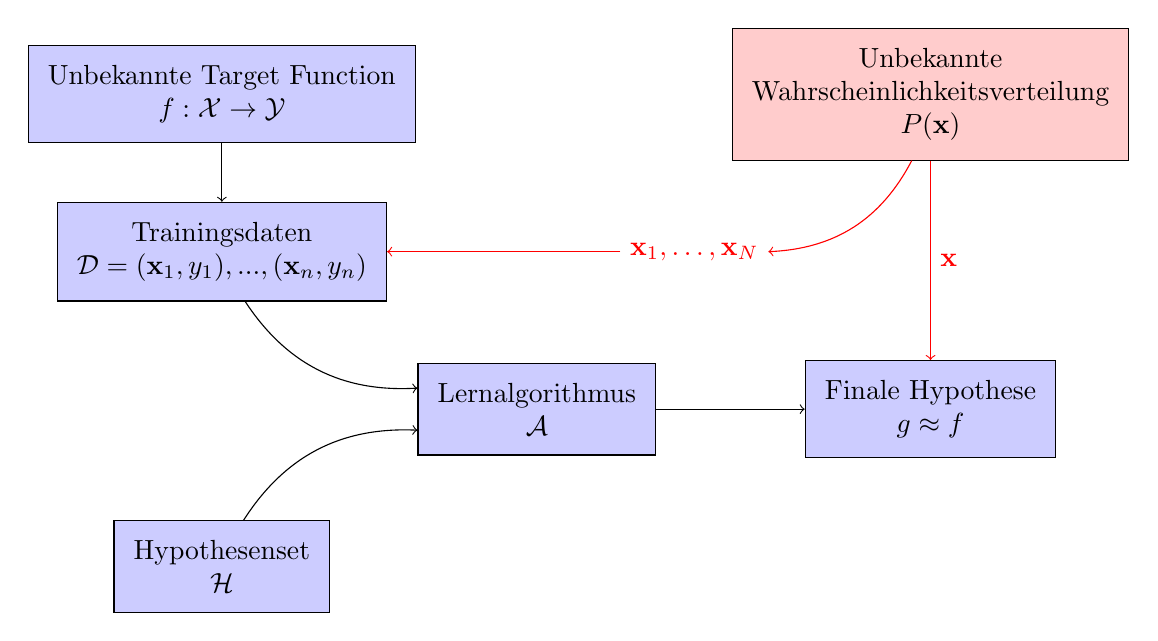
\begin{tikzpicture}
            [myBox/.style={rectangle,
                        draw,
                        align=center,
                        inner sep=2.5mm}]

            \node[myBox, fill=blue!20] (unknownTargetFunction) at (-4, 4) {Unbekannte Target Function\\$f: \mathcal{X} \rightarrow \mathcal{Y}$};
            \node[myBox, fill=blue!20] (trainingExamples) at (-4, 2) {Trainingsdaten\\$\mathcal{D} = (\mathbf{x}_1,y_1),...,(\mathbf{x}_n,y_n)$};
            \node[myBox, fill=blue!20] (learningAlgorithm) at ( 0, 0) {Lernalgorithmus\\$\mathcal{A}$};
            \node[myBox, fill=blue!20] (finalHypothesis) at ( 5, 0) {Finale Hypothese\\$g \approx f$};
            \node[myBox, fill=blue!20] (hypothesisSet) at (-4,-2) {Hypothesenset\\$\mathcal{H}$};

            \node[myBox, fill=red!20] (probabilityDistribution) at (5,4) {Unbekannte\\Wahrscheinlichkeitsverteilung\\$P(\mathbf{x})$};

            \node[red] (x) at (2, 2) {$\mathbf{x}_1, \ldots, \mathbf{x}_N$};

            \draw [->] (unknownTargetFunction) to (trainingExamples);
            \draw [->] (trainingExamples) to [bend right] (learningAlgorithm.170);
            \draw [->] (hypothesisSet) to [bend left] (learningAlgorithm.190);
            \draw [->] (learningAlgorithm) to (finalHypothesis);

            \draw [->, red] (probabilityDistribution) to [bend left] (x.east);
            \draw [->, red] (x) to (trainingExamples);
            \draw [->, red] (probabilityDistribution) to node [midway, right] {$\mathbf{x}$} (finalHypothesis) ;

            %\node[draw,dashed,red,inner sep=2mm,label={[text=red]below:Lernmodell},fit=(learningAlgorithm) (hypothesisSet)] {};
        \end{tikzpicture}
    \end{center}
\end{bonus}

\begin{defi}{Target Verteilung}
    Eine \emph{Target Verteilung} unterscheidet sich dahingehend von einer Target Function, dass sie nicht zwangsläufig deterministisch ist.

    Targets können zufällige Anteile haben (mit \emph{Rauschen} kontaminiert sein).
    Dann ist $y$ eine Zufallsvariable, die von $\mathbf{x}$ abhängt:
    \[
        y = P(y \mid \mathbf{x})
    \]

    Eine Target Function ist also eine deterministische Target Verteilung (also ohne Rauschen).

    Die Datenpunkte einer Target Verteilung entstehen durch Sampeln der multivariaten Verteilung
    \[
        P(\mathbf{x}, y) = P(\mathbf{x}) P(y \mid \mathbf{x})
    \]
\end{defi}

\begin{bonus}{Darstellung des Lernproblems}

    \begin{center}
        % https://tex.stackexchange.com/a/224623/243801
        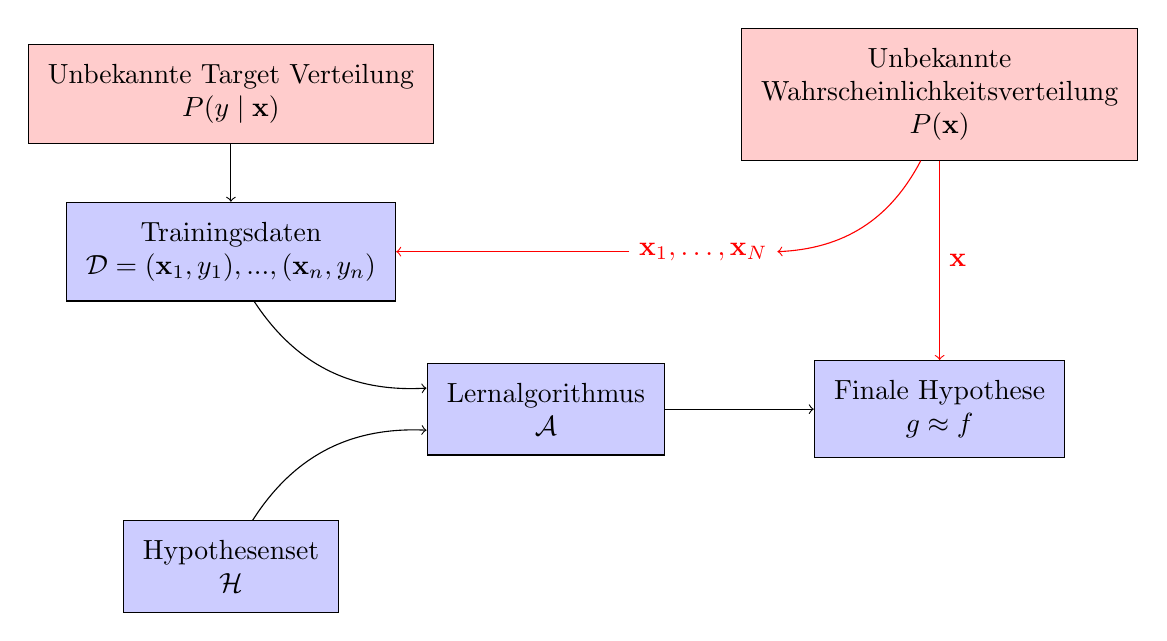
\begin{tikzpicture}
            [myBox/.style={rectangle,
                        draw,
                        align=center,
                        inner sep=2.5mm}]

            \node[myBox, fill=red!20] (unknownTargetDistribution) at (-4, 4) {Unbekannte Target Verteilung\\$P(y \mid \mathbf{x})$};
            \node[myBox, fill=blue!20] (trainingExamples) at (-4, 2) {Trainingsdaten\\$\mathcal{D} = (\mathbf{x}_1,y_1),...,(\mathbf{x}_n,y_n)$};
            \node[myBox, fill=blue!20] (learningAlgorithm) at ( 0, 0) {Lernalgorithmus\\$\mathcal{A}$};
            \node[myBox, fill=blue!20] (finalHypothesis) at ( 5, 0) {Finale Hypothese\\$g \approx f$};
            \node[myBox, fill=blue!20] (hypothesisSet) at (-4,-2) {Hypothesenset\\$\mathcal{H}$};

            \node[myBox, fill=red!20] (probabilityDistribution) at (5,4) {Unbekannte\\Wahrscheinlichkeitsverteilung\\$P(\mathbf{x})$};

            \node[red] (x) at (2, 2) {$\mathbf{x}_1, \ldots, \mathbf{x}_N$};

            \draw [->] (unknownTargetDistribution) to (trainingExamples);
            \draw [->] (trainingExamples) to [bend right] (learningAlgorithm.170);
            \draw [->] (hypothesisSet) to [bend left] (learningAlgorithm.190);
            \draw [->] (learningAlgorithm) to (finalHypothesis);

            \draw [->, red] (probabilityDistribution) to [bend left] (x.east);
            \draw [->, red] (x) to (trainingExamples);
            \draw [->, red] (probabilityDistribution) to node [midway, right] {$\mathbf{x}$} (finalHypothesis) ;

            %\node[draw,dashed,red,inner sep=2mm,label={[text=red]below:Lernmodell},fit=(learningAlgorithm) (hypothesisSet)] {};
        \end{tikzpicture}
    \end{center}

\end{bonus}

\subsection{Lineare Klassifikation und Regression}

\begin{defi}{Arten von Supervised Learning}
    Wir unterscheiden zwischen drei Arten des Supervised Learning, die sich in ihrer Target Function $f$ unterscheiden:
    \begin{itemize}
        \item \emph{Klassifikation}: $f$ bildet auf diskrete Klassen ab
        \item \emph{Regression}: $f$ bildet auf relle Zahlen ab
        \item \emph{Logistische Regression}: $f$ bildet auf Wahrscheinlichkeiten ab
    \end{itemize}
\end{defi}

\begin{defi}{Lineares Modell}
    \emph{Lineare Modelle} kombinieren Features linear miteinander:
    \[
        \theta (s(\mathbf{x})) = \theta \left( \sum_{i=0}^d w_i x_i \right) = \theta (\mathbf{w}^T \mathbf{x})
    \]

    Man unterscheidet zwischen:
    \begin{itemize}
        \item \emph{Lineare Klassifikation}:
              \begin{itemize}
                  \item $\theta$ bildet ab in verschiedene Klassen.
                  \item Beispiel: $\theta(\cdot) = \sign(\cdot)$
              \end{itemize}
        \item \emph{Lineare Regression}:
              \begin{itemize}
                  \item $\theta$ bildet ab in die reellen Zahlen.
                  \item Beispiel: $\theta(\cdot) = \id(\cdot) = \cdot$
              \end{itemize}
        \item \emph{Lineare Logistische Regression}:
              \begin{itemize}
                  \item $\theta$ bildet ab in die rellen Zahlen im Intervall $[0,1]$.
                  \item Beispiel: $\theta(\cdot) = \frac{e^s}{1+e^s}$ (Logistische Funktion)
              \end{itemize}
    \end{itemize}
\end{defi}

\begin{defi}{Lineare Regression}
    Die unbekannte Target Function sei eine bedingte Wahrscheinlichkeitsverteilung $P(y \mid x)$ statt einer deterministischen Target Function $y = f(\mathbf{x})$.

    Wir nehmen an, dass eine \emph{lineare Kombination} der Features $\mathbf{x}$ die Target Function approximiert.

    Die Datenpunkte sollten also möglichst wenig von einer optimalen Hypothese abweichen\footnote{Wir betrachten die quadratische Abweichung (\enquote{Methode der kleinsten Quadrate}).}.

    Dabei stammt $h(\mathbf{x})$ aus dem Hypothesenset $\mathcal{H}$ mit Hypothesen der Form:
    \[
        \mathcal{H}: h(\mathbf{x}) = \sum_{i=0}^d w_i x_i \ \text{mit} \ \mathbf{x} \in \{ 1 \} \times \R^d \ \text{und} \ w \in \R^{d+1}
    \]

    Out-of-Sample Error:
    \[
        E_\text{out}(h) = \Mean((h(\mathbf{x}) - y)^2)
    \]

    In-Sample Error (mit $\displaystyle \mathbf{X} = \vektor{\mathbf{x}_1^T \\ \ldots \\ \mathbf{x}_N^T} \in \R^{N\times (d+1)}$ und $\displaystyle \mathbf{y} = \vektor{y_1 \\ \ldots \\ y_N} \in \R^{N}$):
    \[
        E_\text{in}(\mathbf{w}) = \frac{1}{N} \sum_{i=1}^N ( \mathbf{w}^T \mathbf{x}_i) - y_i)^2 = \frac{1}{N} \cdot \norm{\mathbf{X} \mathbf{w} - \mathbf{y}}^2
    \]

    Gefunden werden soll also ein $\mathbf{w}$, sodass $E_\text{in}$ minimal ist.\footnote{$\mathbf{w}_\text{lin} = \arg\min_\mathbf{w} E_\text{in}(\mathbf{w})$}
    % \[
    %     \mathbf{w}_\text{lin} = \arg\min_\mathbf{w} E_\text{in}(\mathbf{w})
    % \]

    Es gilt (wobei $\mathbf{X}^\dagger$ die Pseudoinverse von $\mathbf{X}$ ist):
    \[
        \mathbf{w}_\text{lin} = \mathbf{X}^\dagger \mathbf{y} = (\mathbf{X}^T \mathbf{X})^{-1} \mathbf{X}^T \mathbf{y}
    \]
\end{defi}

\begin{defi}{Polynomielle Regression}
    Die \emph{polynomielle Regression} ist eine Form der Regressionsanalyse, bei der die Beziehung zwischen des Feature Vectors $\mathbf{x}$ und des Targets $y$ als Polynom $n$-ten Grades in $\mathbf{x}$ modelliert wird.
    Die polynomielle Regression passt eine nichtlineare Beziehung zwischen dem Wert von $\mathbf{x}$ und dem entsprechenden bedingten Mittelwert von $y$ an, bezeichnet als $\Mean(y \mid \mathbf{x})$.

    Obwohl die polynomiale Regression ein nichtlineares Modell an die Daten anpasst, ist sie als statistisches Schätzproblem linear in dem Sinne, dass die Regressionsfunktion $\Mean(y \mid \mathbf{X})$ linear in den unbekannten Parametern ist, die aus den Daten geschätzt werden.

    Aus diesem Grund wird die polynomiale Regression als ein Spezialfall der multiplen linearen Regression betrachtet.

    Der $\mathcal{Z}$-Raum ist dann der Feature Space der transformierten Variable $\Phi(x)$.
    Dabei ist $\Phi(x)$ eine Feature Transform, die $x$ als $\tilde{d}$-dimensionales Polynom modelliert.

    Es gilt also:
    \[
        \mathcal{Z}: \Phi(x) \in \{ 1 \} \times \R^{\tilde{d}}
    \]
\end{defi}

\subsection{Approximation versus Generalisierung}

\begin{defi}{Approximation}
    Das Ziel der \emph{Approximation} ist es, einen möglichst kleinen In-Sample Error $E_\text{in}$ auf dem Trainingsset zu erhalten.
\end{defi}

\begin{defi}{Generalisierung}
    Das Ziel der \emph{Generalisierung} ist es, einen Out-of-Sample Error $E_\text{out}$ zu erhalten, der annähernd dem In-Sample Error $E_\text{in}$ entspricht:
    \[
        E_\text{out}(h) \approx E_\text{in}(h)
    \]
\end{defi}

\begin{defi}{Approximations-Generalisierungsabwägung}
    Approximation und Generalisierung stehen im \emph{Konflikt}.

    In der Praxis ist oft entweder
    \begin{itemize}
        \item \emph{perfekte Approximation} und \emph{schlechte Generalisierung}, oder
        \item \emph{sehr gute Generalisierung} aber \emph{schlechte Approximation}
    \end{itemize}
    zu beobachten.

    Einflussfaktoren für diesen Konflikt sind beispielsweise:
    \begin{itemize}
        \item Komplexität des Lernmodells (Modellkomplexität)
        \item Anzahl der Trainingsdatenpunkte (Datenmenge)
        \item Kontamination der Daten mit Rauschen (Rauschkontamination)
    \end{itemize}
\end{defi}

\begin{bonus}{Approximations-Generalisierungsabwägung}
    Ergebnis der statistischen Lerntheorie:
    \[
        E_\text{out}(g) \leq E_\text{in}(g) + \Omega (N, \mathcal{H})
    \]
    Dabei ist $\Omega$ ein Strafterm, der eine hohe Modellkomplexität bestraft.

    \begin{center}
        % https://tex.stackexchange.com/a/563020/243801
        \tikzset{>=stealth,
            OptimumStyle/.style={align=center,anchor=east,rotate=90,font=\sffamily\scriptsize}
        }
        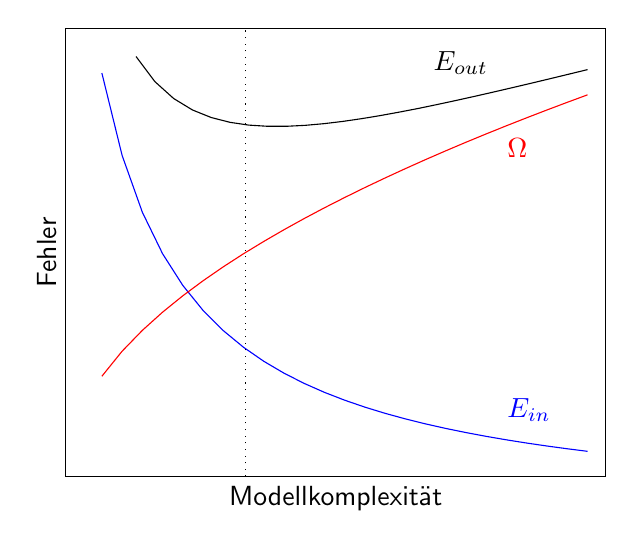
\begin{tikzpicture}[font=\sffamily]
            \begin{axis}[
                    xmin= 0,
                    xmax= 3,
                    ymin= 0,
                    ymax= 2,
                    xlabel=Modellkomplexität,
                    ylabel=Fehler,
                    ticks=none,
                    xticklabels={\empty},
                    yticklabels={\empty}
                ]
                \addplot[domain=0.2:2.9,blue] {1/(x+0.3)-0.2};   %In-Sample Error
                \addplot[domain=0.2:2.9,red] {x^(1/2)};   %Penalty
                \addplot[domain=0.39:2.9,black] {x^(1/2) + 1/(x+0.3)-0.2};  %Out-of-Sample Error
                \addplot[dotted,thin] coordinates {(1,0) (1,2)};       %Optimum model complexity
                %\node[OptimumStyle] at (axis cs:0.9,2) {optimale\\Modellkomplexität};
                \node[anchor=south west,text=blue] at (axis cs:2.4,0.2){$E_\text{in}$};
                \node[anchor=north west,text=red] at (axis cs:2.4,1.55){$\Omega$};
                \node[anchor=south east,align=center] at (axis cs:2.4,1.75){$E_\text{out}$};
                \legend{}
            \end{axis}
        \end{tikzpicture}
    \end{center}

    \begin{itemize}
        \item Links der optimalen Modellkomplexität findet \emph{Underfitting} statt.
        \item Rechts der optimalen Modellkomplexität findet \emph{Overfitting} statt.
    \end{itemize}
\end{bonus}

\begin{defi}{Bias}
    Für verschiedene Datensätze $\mathcal{D}$ desselben Lernproblems erhalten wir verschiedene finale Hypothesen $g$.

    Der \emph{Bias} bzw. die \emph{Verzerrung} misst die Abweichung zwischen der über allen möglichen Datensätzen gemittelten finalen Hypothese $g$ und der Target Function $f$.

    Er charakterisiert weiterhin, wie stark unser Lernmodell (Hypothesenset und Algorithmus) von der Target Function prinzipiell abweicht.
\end{defi}

\begin{defi}{Varianz}
    Die \emph{Varianz} misst, wie stark eine durch einen gewählen Datensatz $\mathcal{D}$ gewonnene finale Hypothese um die mittlere finale Hypothese streut.

    Sie kann als Instabilität des Lernmodells interpretiert werden.
    Instabilität zeigt sich in großen Reaktionen des Lernmodells auf kleine Variationen in Datensätzen.

    Wächst die Größe der Datensätze, wird die Varianz kleiner.
\end{defi}

\begin{bonus}{Visualisierung Bias, Varianz}
    % https://tex.stackexchange.com/a/307285/243801
    \begin{center}
        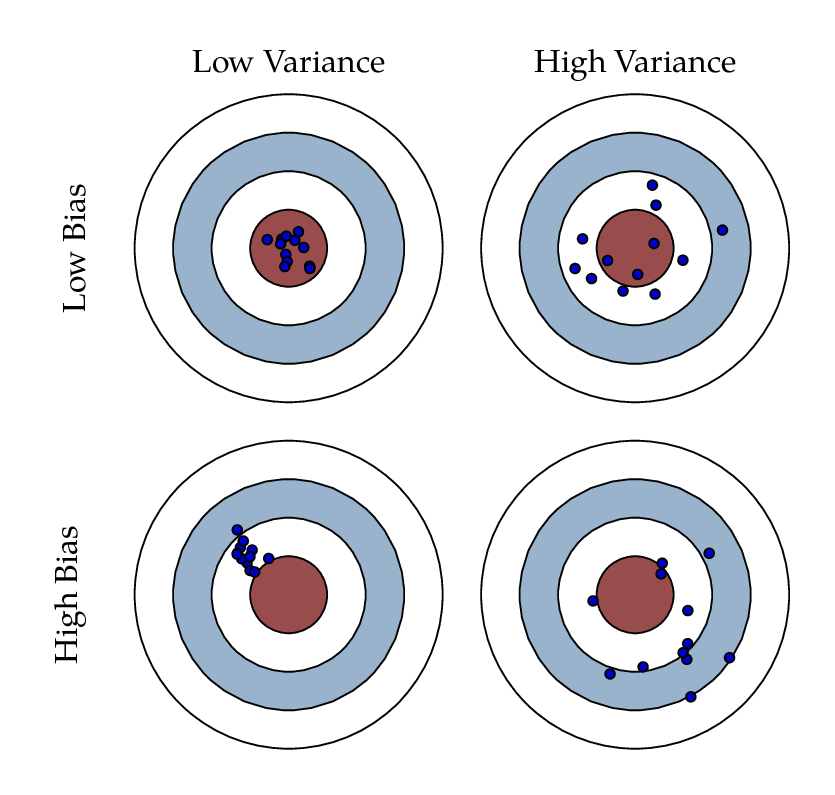
\includegraphics[width=.7\textwidth]{includes/figures/bonus_defi_variance.png}
    \end{center}
\end{bonus}

\begin{defi}{Bias-Variance Tradeoff}
    \begin{center}
        % https://tex.stackexchange.com/a/563020/243801
        \tikzset{>=stealth,
            OptimumStyle/.style={align=center,anchor=east,rotate=90,font=\sffamily\scriptsize}
        }
        \begin{tikzpicture}[font=\sffamily]
            \begin{axis}[
                    xmin= 0,
                    xmax= 2,
                    ymin= 0,
                    ymax= 2,
                    xlabel=Modellkomplexität,
                    ylabel=Fehler,
                    ticks=none,
                    xticklabels={\empty},
                    yticklabels={\empty}
                ]
                \addplot[domain=0.2:1.9,red] {1/(x+0.3)-0.2};   %Bias
                \addplot[domain=0.2:1.9,blue] {0.12*e^(1.40*x)};   %Variance
                \addplot[domain=0.39:1.61,black] {3*(x-2)*x+3.8};  %Total error
                \addplot[dotted,thin] coordinates {(1,0) (1,2)};       %Optimum model complexity
                \node[OptimumStyle] at (axis cs:0.9,2) {optimale\\Modellkomplexität};
                \node[anchor=south west,text=red] at (axis cs:1.4,0.4){Bias};
                \node[anchor=north west,text=blue] at (axis cs:1.4,0.85){Varianz};
                \node[anchor=south east,align=center] at (axis cs:1.5,1.5){$E_\text{out}$};
                \legend{}
            \end{axis}
        \end{tikzpicture}
    \end{center}
\end{defi}

\begin{defi}{Overfitting}
    \emph{Overfitting} ist der Prozess, Hypothesen $h$ mit kleinerem In-Sample Error $E_\text{in}$ zu wählen, die zu wachsendem Out-of-Sample Error $E_\text{out}$ führen.

    Wir beobachten Overfitting für eine Hypothese $h$, wenn es eine weitere Hypothese $h'$ gibt, so dass gilt:
    \[
        E_\text{in}(h) \leq E_\text{in}(h') \ \text{aber} \ E_\text{out}(h) \geq E_\text{out}(h')
    \]

    Overfitting hängt davon ab, wie die gewählte Modellkomplexität zur Quantität und Qualität der Daten passt (und nicht, wie die gewählte Modellkomplexität zur Komplexität der Target Functionpasst).

    Es gilt:
    \begin{itemize}
        \item mehr Datenpunkte \emph{reduzieren} die Tendenz zu Overfitting
        \item mehr Rauschkontamination \emph{erhöht} die Tendenz zu Overfitting
        \item höhere Target Komplexität \emph{erhöht} die Tendenz zu Overfitting
    \end{itemize}
\end{defi}

\subsection{Regularisierung}

\begin{defi}{Regularisierung}
    \emph{Regularisierung} schränkt den Lernalgorithmus ein, um den Out-Of-Sample Error $E_\text{out}$ zu verbessern und Overfitting zu bekämpfen.\footnote{Aus einem ähnlichen Grund erfordert eine höhere Rauschkontamination auch eine stärkere Regularisierung.}

    Regularisierungstechniken sind meist heuristische Methoden;
    es fehlt oft eine mathematische Begründung, warum sie funktionieren.

    Aus dem bekannten Strafterm für Modellkomplexität in
    \[
        E_\text{out}(h) \leq E_\text{in} + \Omega(N, \mathcal{H}) \ \text{für alle} \ h \in \mathcal{H}
    \]
    sieht man:
    \begin{itemize}
        \item Wahl eines \emph{einfachen} Hypothesensets $\mathcal{H}$ verbessert die Schranke (geringere Modellkomplexität).
        \item Wahl einer \emph{einfachen Hypothese} $h \in \mathcal{H}$ verbessert die Schranke (Komplexität der Hypothese $\Omega(h)$ wird klein).
    \end{itemize}

    Regularisierung zielt darauf ab, einfache Hypothesen aus dem Hypothesenset zu wählen:
    \begin{itemize}
        \item Minimiere $E_\text{in}(h)$ und $\Omega(h)$ \emph{gleichzeitig}.
    \end{itemize}

    Regularisierung reduziert den Varianz-Term, doch der Bias-Term steigt an:
    \enquote{Wir tauschen den niedrigen Bias-Term gegen eine deutliche Verkleinerung des Varianz-Terms ein.}
    \footnote{Typisch für die Praxis: Nutzung eines komplexen Hypothesensets + Regularisierung ergibt die kleinsten Out-of-Sample Error $E_\text{out}$.}
\end{defi}

\begin{defi}{Augmented Error}
    Regularisierung kann durch den \emph{Augmented Error} bzw. \emph{erweiterten Fehler} $E_\text{aug}$ mit freiem Parameter $\lambda \geq 0$ stattfinden:
    \[
        E_\text{aug}(\mathbf{w}) = E_\text{in}(\mathbf{w}) + \frac{\lambda}{N} \underbrace{\mathbf{w}^T \mathbf{w}}_{\text{Strafterm} \ \Omega(h)}
    \]

    Dabei stellt das $\lambda$ ein, \enquote{wie stark} die Regularisierung sein soll.
    \footnote{
        Der Faktor $\nicefrac{1}{N}$ ist eingebaut, da mit mehr Datenpunkten weniger Regularisierung notwendig ist.
        Das ist nur eine Redefinition von $\lambda$.
    }

    Wir erwarten stärkere Regularisierung und bessere Generalisierung, wenn $\lambda$ ansteigt.
\end{defi}

\begin{defi}{Weight Decay}
    Das Ziel von \emph{Weight Decay} ist es, große Gewichte zu verhindern und dadurch \enquote{glattere} Hypothesen zu erzeugen.

    Explizit nutzen wir Weight Decay mit
    \[
        \Omega(h) = \mathbf{w}^T \mathbf{w}
    \]

    Insbesondere ist Rauschen auch meist \enquote{nicht glatt} bzw. hochfrequent.
    Dadurch schadet die Regularisierung mit Weight Decay dem Overfitting mehr als der Fähigkeit, das Signal in den Daten zu fitten.
\end{defi}

\begin{defi}{Lineare Regression mit Weight Decay}
    %Sei $\mathbf{Z} = \vektor{\mathbf{z}_1^T \\ \mathbf{z}_2^T \\ \vdots \\ \mathbf{z}_N^T}$.

    Lineare Regression ohne Regularisierung:
    \begin{itemize}
        \item Finde $\mathbf{w}_\text{lin}$, das $E_\text{in}$ minimiert:
              \[
                  E_\text{in}(\mathbf{w}) = \frac{1}{N} (\mathbf{Z}\mathbf{w} - \mathbf{y})^T (\mathbf{Z}\mathbf{w} - \mathbf{y})
              \]
              \[
                  \mathbf{w}_\text{lin} = \arg\min_\mathbf{w} E_\text{in}(\mathbf{w}) = (\mathbf{Z}^T \mathbf{Z})^{-1} \mathbf{Z}^T \mathbf{y}
              \]
    \end{itemize}

    Lineare Regression mit Regularisierung:
    \begin{itemize}
        \item Finde $\mathbf{w}_\text{aug}$, das $E_\text{aug}$ minimiert:
              \[
                  E_\text{aug}(\mathbf{w}) = E_\text{in}(\mathbf{w}) + \frac{\lambda}{N} \mathbf{w}^T \mathbf{w}
              \]
              \[
                  \mathbf{w}_\text{aug} = \arg\min_\mathbf{w} E_\text{aug}(\mathbf{w}) = (\mathbf{Z}^T \mathbf{Z} + \lambda \mathbf{I})^{-1} \mathbf{Z}^T \mathbf{y}
              \]
    \end{itemize}
\end{defi}

\subsection{Validierung}

\begin{defi}{Validierung}
    \emph{Validierungstechniken} werden genutzt
    \begin{itemize}
        \item zur Schätzung des Out-of-Sample Errors $E_\text{out}$
        \item zur Wahl von Modellen bzw. zur Bestimmung von Hyperparametern, z.B.
              \begin{itemize}
                  \item Parameter, die die Modellarchitektur bestimmen
                  \item Parameter, die den Lernalgorithmus betreffen
                  \item \emph{Regularisierungsparameter}
              \end{itemize}
    \end{itemize}
\end{defi}

\begin{bonus}{Lernkurve}
    \begin{center}
        \begin{tikzpicture}[font=\sffamily]
            \begin{axis}[
                    xmin= 0.4,
                    xmax= 5,
                    ymin= -2,
                    ymax= 2,
                    xlabel=Trainingsdatenpunktanzahl,
                    ylabel=Fehler,
                    ticks=none,
                    xticklabels={\empty},
                    yticklabels={\empty}
                ]
                \addplot[name path=Eout, domain=0.6:4.8,red] {1/x}; %E_out
                \addplot[name path=Ein, domain=0.6:4.8,blue] {-1/x}; %E_in

                \path[name path=axis, draw=none] (axis cs:0.6,-1.8) -- (axis cs:4.8,-1.8);

                % color between E_in and E_out
                \addplot[fill=red, fill opacity = 0.1, domain=0.6:4.8] fill between[of=Ein and Eout];
                \addplot[fill=blue, fill opacity = 0.1, domain=0.6:4.8] fill between[of=Ein and axis];
                \addplot[domain=0.6:4.8,black] {0}; %middle

                \node[anchor=south east,align=center, text=red] at (axis cs:4.5,0.5){$E_\text{out}$};
                \node[anchor=south east,align=center, text=blue] at (axis cs:4.5,-1){$E_\text{in}$};
                \legend{}
            \end{axis}
        \end{tikzpicture}
    \end{center}
\end{bonus}

\subsubsection{Schätzen des Out-of-Sample Errors}

\begin{defi}{Hold-Out Validierung (Schätzen des Out-of-Sample Errors)}
    Bei der \emph{Hold-Out Validierung} werden die Daten $\mathcal{D}$ zufällig in Trainingsset $\mathcal{D}_\text{train}$ ($N-K$ Datenpunkte) und Validierungsset $\mathcal{D}_\text{val}$ ($K$ Datenpunkte) aufgeteilt.
    \footnote{Typisch in der Praxis ist $K = \nicefrac{N}{5}$.}

    Die finale Hypothese $g^{-} \in \mathcal{H}$ wird dann auf dem Trainingsset erhalten.

    Der \emph{Validierungsfehler} $E_\text{val}$ wird dann mithilfe von $g^{-}$ auf dem Validierungsset $\mathcal{D}_\text{val}$ berechnet.

    Typisch ist folgendes Vorgehen:
    \begin{enumerate}
        \item Berechne Validierungsfehler und nutze $E_\text{val}$ als Schätzer für $E_\text{out}$.
        \item Bestimme finale Hypothese $g$ auf dem \emph{ganzen} Datensatz $\mathcal{D}$ (Retraining) und liefere $g$ aus.
    \end{enumerate}

    Hold-Out Validierung ist generell wenig rechenintensiv, da nur ein Modell trainiert werden muss.
\end{defi}

\begin{defi}{Leave-One-Out Kreuzvalidierung (LOO-CV) (Schätzen des Out-of-Sample Errors)}
    Bei der \emph{Leave-One-Out Kreuzvalidierung} (LOO-CV) werden die Daten $\mathcal{D}$ zufällig in Trainingsset mit $N-1$ Datenpunkten und Validierungsset mit einem Datenpunkt aufgeteilt.

    Sei $\mathcal{D}_n := \mathcal{D} \setminus (\mathbf{x}_n, y_n)$ und die auf $\mathcal{D}_n$ gelernte Hypothese $g^{-}_n \in \mathcal{H}$.

    Dann sei der punktweise Fehler auf dem Validierungsset $\{ \mathbf{x}_n, y_n \}$:
    \[
        e_n := E_\text{val}(g^{-}_n) = e(g^{-}_n(\mathbf{x}_n), y_n)
    \]

    Der gesamte Kreuzvalidierungsfehler $E_\text{CV}$ ist dann:
    \[
        E_\text{CV} = \frac{1}{N} \sum_{n=1}^N e_n
    \]

    Vorgehen:
    \begin{enumerate}
        \item Erzeuge $N$ Datensätze $\mathcal{D}_n$ aus dem Datensatz $\mathcal{D}$ mit $N$ Datenpunkten.
        \item Ermittle die finalen Hypothesen für jeden Datensatz $\mathcal{D}_n$.
        \item Erhalte den Kreuzvalidierungsfehler $E_\text{CV}$ als Mittelwert der Validierungsfehler $e_n$.
    \end{enumerate}

    LOO-CV ist generell sehr rechenintensiv, da $N$ Modelle trainiert werden müssen.
\end{defi}

\begin{defi}{V-fache Kreuzvalidierung (Schätzen des Out-of-Sample Errors)}
    Bei der \emph{V-fachen Kreuzvalidierung} werden die Daten $\mathcal{D}$ in $V$ gleich große disjunkte Teilmengen bzw. \emph{Folds} $\mathcal{D}_v$ aufgeteilt.
    Typische Werte für $V$ sind z.B. $5$ oder $10$.

    Für alle $v = 1, \ldots, V$ wird dann ein Modell auf $\mathcal{D} \setminus \mathcal{D}_v$ trainiert und der Validierungsfehler $E_v$ auf $\mathcal{D}_v$ berechnet.

    Der gesamte Kreuzvalidierungsfehler $E_\text{V-fold CV}$ ist dann:
    \[
        E_\text{V-fold CV} = \frac{1}{V} \sum_{v=1}^V E_v
    \]

    Von der Wahl von $V$ ist abhängig:
    \begin{itemize}
        \item Anzahl Datenpunkte im Trainingsset $N_\text{train} = \frac{V-1}{V} N$
        \item Anzahl Datenpunkte im Validierungsset $N_\text{val} = \frac{1}{V} N$
        \item Bias:
              \subitem kleines $V$
              \subitem $\implies$ $N_\text{train} \ll N$
              \subitem $\implies$ großer Bias für $E_\text{V-fold CV}$
              \subitem (Schätzer für $E_\text{out}$ bei $N_\text{train}$ Daten, interessieren uns aber für $N$ Daten)
        \item Varianz:
              \subitem großes $V$
              \subitem $\implies$ $N_\text{train} \approx N$ und $N_\text{val} \to 1$
              \subitem $\implies$ große Varianz für $E_\text{V-fold CV}$
              \subitem (verschiedene $g^{-}_n$ sind hochkorreliert, da Trainingsdaten fast identisch)
              \subitem $\implies$ Fehler $E_v$ sind stark korreliert.
    \end{itemize}
\end{defi}

\subsubsection{Modellauswahl}

\begin{defi}{Modellauswahl}
    Der wichtigste Anwendungsfall für Validierungstechniken ist die \emph{Modellauswahl} (\emph{model selection}) bzw. die Bestimmung von Hyperparametern.

    Die Idee:
    \begin{itemize}
        \item Nutze Validierung, um $E_\text{out}$ für \emph{mehrere Modelle} zu schätzen.
        \item Wähle das Modell mit der kleinsten Schätzung für $E_\text{out}$ aus.
    \end{itemize}

    Modelle können z.B. sein:
    \begin{itemize}
        \item Polynome mit unterschiedlicher Ordnung $Q$
        \item Ein Modell mit unterschiedlich starker Regularisierung $\lambda$: $(\mathcal{H}, \lambda_1), (\mathcal{H}, \lambda_2), \ldots, (\mathcal{H}, \lambda_M)$
    \end{itemize}
\end{defi}

\begin{defi}{Hold-Out Validierung (Modellauswahl)}
    Vorgehen:
    \begin{enumerate}
        \item Betrachte $M$ Modelle bzw. Hypothesensets $\mathcal{H}_1, \ldots, \mathcal{H}_M$
        \item Erhalte finale Hypothesen auf dem Trainingset: $g^{-}_1, \ldots, g^{-}_M$
        \item Errechne den Validierungsfehler $E_\text{val}$ als Schätzer für $E_\text{out}$ für jedes der $M$ Modelle:
              \[
                  E_\text{val}(m) = E_\text{val}(g^{-}_m), \, m \in 1, \ldots, M
              \]
        \item Selektiere bestes Modell $m^*$ mit dem kleinsten Validierungsfehler $E_m^*$
        \item Bestimme finale Hypothese $g$ des Modells $m^*$ auf dem ganzen Datensatz
    \end{enumerate}

    Der Validierungsfehler $E_\text{val}(g^{-}_m)$ wird zur Auswahl des finalen Modells genutzt und ist daher \enquote{optimistisch} verzerrt.
    Das hat zur Folge, dass der optimistische Validierungsfehler tendenziell niedriger ist als der wahre Out-of-Sample Error $E_\text{out}$.

    \emph{Wichtig}:
    Je mehr Lernentscheidungen über das Validierungsset getroffen werden, desto schlechter kann $E_\text{val}$ Aussagen über $E_\text{out}$ treffen und desto mehr wird das Validierungsset zum Traininsset.
\end{defi}

\begin{defi}{Leave-One-Out Kreuzvalidierung (LOO-CV) (Modellauswahl)}
    Vorgehen (bei der Auswahl des Regularisierungsparameters $\lambda$):
    \begin{enumerate}
        \item Definiere $M$ Modelle $(\mathcal{H}, \lambda_1), (\mathcal{H}, \lambda_2), \ldots, (\mathcal{H}, \lambda_M)$
        \item Bestimme für jedes Modell $m = 1, \ldots, M$ den Kreuzvalidierungsfehler $E_\text{CV}(m)$
        \item Selektiere bestes Modell $m^*$ mit dem kleinsten Kreuzvalidierungsfehler $E_\text{CV}$
        \item Nutze $(\mathcal{H}, \lambda_{m^*})$ und alle Daten $\mathcal{D}$, um die finale Hypothese $g_m^*$ zu trainieren.
    \end{enumerate}

    Insgesamt müssen hier also $(M \cdot N) + 1$ Modelle trainiert werden.
\end{defi}
\section{Modellierung}

\begin{defi}{Modell}
    Ein \emph{Modell} ist eine Abstraktion eines Systems, die benutzt wird, um ein existierendes System zu beschreiben oder ein neu zu erstellendes System zu spezifizieren.

    Ein Modell wird so konstruiert, dass es anstelle des Originals für den jeweils gegebenen Zweck verwendet werden kann.

    Eigenschaften eines Modells:
    \begin{itemize}
        \item \emph{Abbildung}: Das Modell stellt ein Abbild des zu untersuchenden Systems dar.
        \item \emph{Reduktion}: Das Modell abstrahiert von irrelevanten Eigenschaften und erleichtert damit die Untersuchung des Systems.
        \item \emph{Pragmatik}: Das Modell ist für den jeweiligen Zweck geeignet.
    \end{itemize}
\end{defi}

\begin{example}{Modell}
    \begin{center}
        \raisebox{-0.5\height}{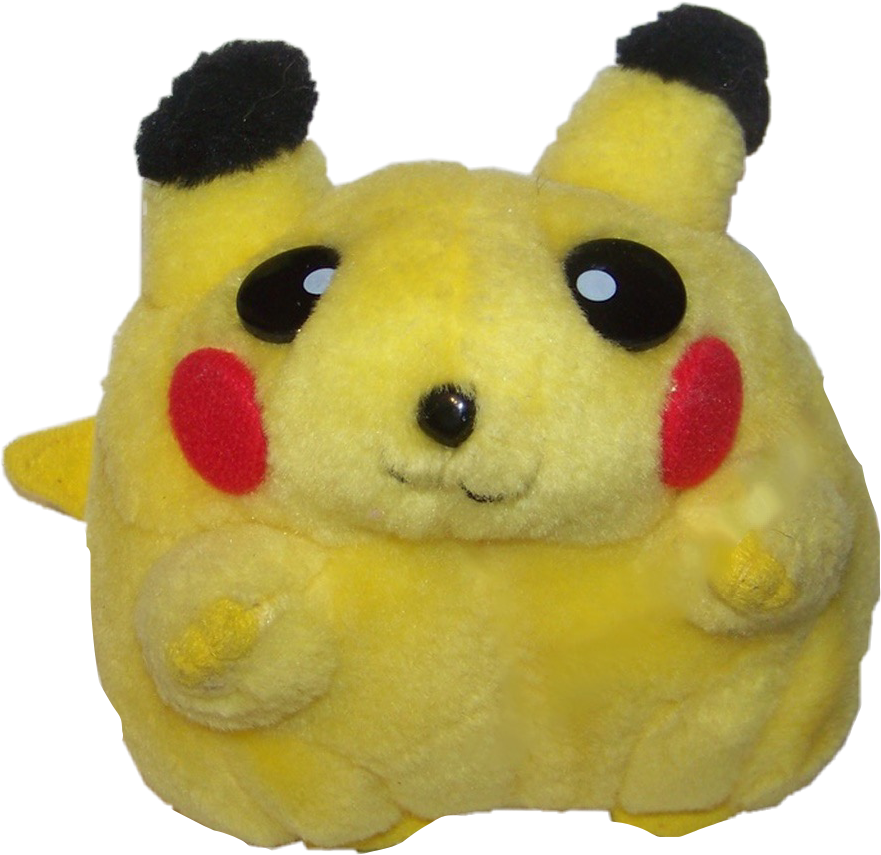
\includegraphics[width=.4\textwidth]{includes/figures/example_modell.png}}
        \hspace{6em}
        \raisebox{-0.5\height}{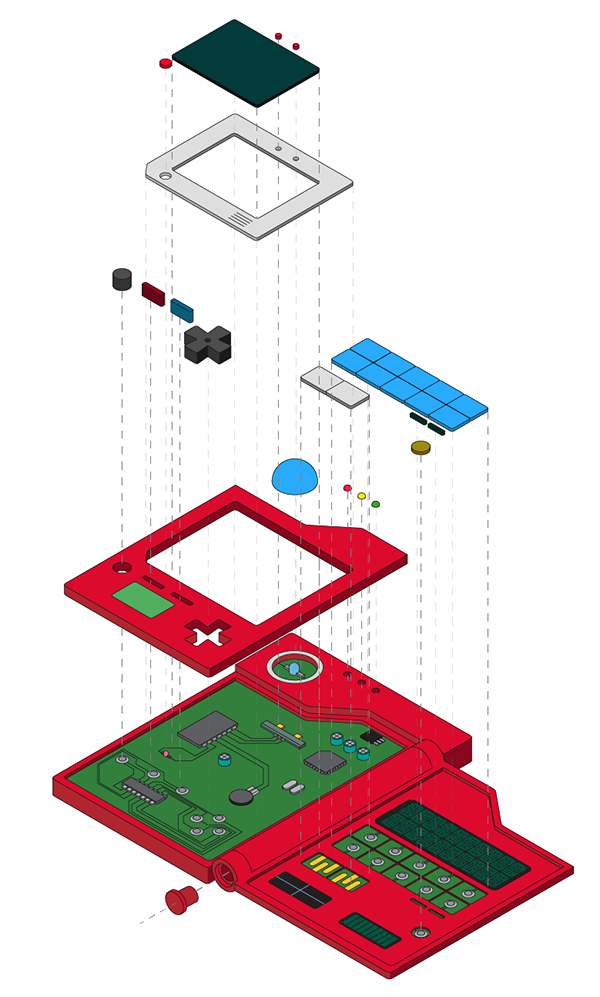
\includegraphics[width=.3\textwidth]{includes/figures/example_modell_2.png}}
    \end{center}
\end{example}

\begin{bonus}{Zweck eines Modells}
    \begin{tabularx}{\textwidth}{|l|X|}
        \hline
        \bfseries Verstehen     & Das Modell erleichtert \emph{mir} durch geeignete Abstraktionen das Verständnis des Systems                                              \\
        \hline
        \bfseries Kommunikation & Das Modell wird dazu verwendet, \emph{anderen Personen} das zugrunde liegende System zu erläutern                                        \\
        \hline
        \bfseries Analyse       & Mit Hilfe des Modells werden \emph{Eigenschaften} des Systems untersucht                                                                 \\
        \hline
        \bfseries Simulation    & Das Modell wird benutzt, um das Verhalten des Systems zu simulieren und dadurch Erkenntnisse über das tatsächliche Verhalten zu gewinnen \\
        \hline
        \bfseries Spezifikation & Das Modell dient als Vorschrift für ein noch zu erstellendes System                                                                      \\
        \hline
        \bfseries Generierung   & Aus dem Modell wird zu erstellende System automatisch erzeugt                                                                            \\
        \hline
    \end{tabularx}
\end{bonus}

\begin{defi}{Präskriptive und deskriptive Modellierung}
    Bei \emph{präskriptiver (vorschreibender) Modellierung} dient das Modell als Spezifikation für die Realisierung (Vorbild).

    Bei \emph{deskriptiver (beschreibender) Modellierung} wird das Modell als Sicht auf ein bereits existierendes System konstruiert (Abbild).
\end{defi}

\begin{defi}{Strukturelles Modell}
    Ein \emph{strukturelles Modell} beschreibt die statische Struktur eines Systems (Elemente und Beziehungen).
\end{defi}

\begin{defi}{Verhaltensmodell}
    Ein \emph{Verhaltensmodell} beschreibt das dynamische Verhalten eines Systems (Ausführung von Operationen, Reihenfolge von Schritten).
\end{defi}

\begin{defi}{Objektorientierte Analyse}
    In der \emph{objektorientierte Analyse} (OOA) geht es darum, die Anforderungen objektorientiert zu erfassen und zu beschreiben, die das zu entwickelnde Softwaresystem erfüllen soll.
    In dieser Phase werden alle Fakten gesammelt, dargestellt und überprüft.
    Dies kann in Form eines textuellen Pflichtenheftes geschehen.

    Ergebnis der objektorientierten Analyse ist ein allgemeines Produktmodell in Form eines objektorientierten Analyse-Modells (OOA-Modell).
    Diese fachliche Beschreibung mit objektorientierten Konzepten enthält verschiedene Artefakte wie Diagramme und Darstellungen von Kontrollstrukturen.
\end{defi}

\begin{defi}{Schritte zum OOA-Modell}
    \begin{enumerate}
        \item Klassen finden
        \item Beziehungen und Aggregationen finden
        \item Klassenkomponenten finden:
              \begin{enumerate}
                  \item Attribute finden
                  \item Externe Operationen finden
              \end{enumerate}
        \item Objekt-Lebenszyklus erstellen
        \item Vererbungsstrukturen finden
        \item Interne Operationen finden
        \item Operationen spezifizieren
        \item Vererbungsstrukturen prüfen
        \item Beziehungen und Aggregationen prüfen
        \item Subsysteme finden
    \end{enumerate}

    Je nach Projektfluss sind auch \emph{Vorgriffe} und \emph{Rückgriffe} oder \emph{Iterationen} denkbar bzw. nötig.

    Neben dem Kern-OO-Modell sollten noch ein \emph{Glossar} und eine \emph{Liste offener Fragen} geführt werden.
\end{defi}

\begin{defi}{Objektorientiertes Design}
    Beim \emph{objektorientierten Design} (OOD) wird das in der objektorientierten Analyse erstellte Domänenmodell weiterentwickelt und darauf aufbauend ein Systementwurf erstellt.
    Dabei wird das allgemeine Modell in eine konkrete Softwarearchitektur umgeformt, die Informationen über Details der technischen Umsetzung enthält und direkt als Vorlage für die Implementierung in einer Programmiersprache dient, die idealerweise objektorientierte Programmierung (OOP) unterstützt.

    Dadurch, dass in den Entwicklungsphasen Analyse und Design bereits objektorientierte Techniken eingesetzt werden, wird der Übergang zur Implementierung in einer objektorientierten Programmiersprache erleichtert.
\end{defi}
\section{Relationale Algebra}

\begin{defi}{Relationale Algebra}
    Eine \emph{relationale Algebra} definiert (Mengen-)Operationen, die sich auf eine Menge von Relationen anwenden lassen.
    Damit können Relationen beispielsweise gefiltert, verknüpft oder aggregiert werden.
    Die Ergebnisse aller Operationen sind ebenfalls Relationen.
    Aus diesem Grund bezeichnet man die Relationenalgebra als abgeschlossen.

    Eine Relation
    \[
        R \subseteq D_1 \times \ldots \times D_n
    \]
    ist wie bisher primär eine konkrete Tupelmenge
    \[
        t = [a_1, \ldots, a_n] \in R, a_k \in D_k
    \]

    Eine Tabelle ist eine visuelle Repräsentation einer Relation und eine Zeile in einer Tabelle repräsentiert ein Tupel.

    Steht die Relation für einen Entitätstyp, so sind die Tupel konkrete Entitäten.
\end{defi}

\begin{bonus}{Funktionen zum Aufbau einer Relation}
    Ist man statt an einer Relation $R$, also der konkreten Tupelmenge, nur am Aufbau der Relation, d.h. den Attributen und Datentypen, interessiert, helfen diese Funktionen:
    \begin{itemize}
        \item $\ident(R) = \{a_i\}$
        \item $\schema(R) = \{[a_1:T_1, \ldots, a_n:T_n]\}$
    \end{itemize}
\end{bonus}

\begin{defi}{Schlüsselkandidat (Relationale Algebra)}
    Ein \emph{Schlüsselkandidat} $K$ mit $K \subseteq \ident(R)$ ist eine Menge von Attributen, deren Werte jeweils alle Tupel der Relation eindeutig identifizieren (\enquote{identifier}).

    So ist implizit garantiert, dass es keine zwei gleichen Tupel in der Relation gibt.

    Grundsätzlich kann es mehrere Schlüsselkandidaten geben, aus denen dann der Schlüssel (\enquote{primary key}) ausgewählt wird.
\end{defi}

\subsection{Mengenoperationen}

\begin{defi}{Voraussetzungen für Mengenoperationen}
    Um Mengenoperationen auf Relationen durchzuführen, müssen diese kompatibel sein.
    Das bedeutet, Attributanzahl und Wertebereiche müssen übereinstimmen (\emph{Vereinigungsverträglichkeit} bzw. \emph{Typkompatibilität}).

    Für zwei Relationen $S$ und $T$ muss also gelten, dass\footnote{Die Attribute müssen allerdings nicht formal gleich heißen, eine verträgliche Semantik ist aber sinnvoll.}
    \[
        \schema(S) = \schema(T)
    \]
\end{defi}

\begin{defi}{Klassische Mengenoperationen}
    Seien $S$ und $T$ zwei kompatible Relationen.
    Dann sind definiert:
    \begin{itemize}
        \item \emph{Vereinigung}:
              \[
                  S \cup T = \{ r \mid r \in S \lor r \in T \}
              \]
        \item \emph{Differenz}:
              \[
                  S - T = S \setminus T = \{ r \mid r \in S \land r \notin T \}
              \]
        \item \emph{Schnittmenge}:
              \[
                  S \cap T = \{ r \mid r \in S \land r \in T \}
              \]
    \end{itemize}

    %Für mehr Informationen und Beispiele zu den konkreten Anwendungen in SQL: %\fullref{SQL}.
\end{defi}

\begin{defi}{Kartesisches Produkt}
    Für zwei Relationen $S$ und $T$ mit
    \[
        \ident(S) \cap \ident(T) = \emptyset
    \]
    ist das \emph{kartesische Produkt} $S \times T$ definiert durch
    \[
        S \times T = \bigcup_{(s_1, \ldots, s_n) \in S} \left[ \bigcup_{(t_1, \ldots, t_k) \in T} \{ (s_1, \ldots,  s_n, t_1, \ldots, t_k) \} \right]
    \]

    Im üblichen kartesisches Produkt entstehen Paare $(s,t)$ mit $s \in S$ und $t \in T$.
    Hier hingegen entstehen $\abs{S \times T} = \abs{S} \cdot \abs{T}$ Tupel, bestehend aus allen Attributen einer Entität $s \in S$ verbunden mit den Attributen einer Entität $t \in T$.

    Im Fall $\ident(S) \cap \ident(T) \neq \emptyset$ würde obige Definition doppelte Attribute erzeugen, was mathematisch ein Problem ist, aber in der Praxis durch Umbenennung der Attribute gelöst werden kann.

    \emph{Eselsbrücke}: Jedes Element von $S$ mit jedem von $T$.
\end{defi}

\begin{defi}{Selektion}
    Für eine Relation $S$ und eine logische Bedingung $\Theta$ ist die \emph{Selektion} definiert durch
    \[
        \sigma_\Theta(S) = \{ s \in S \mid s \ \text{erfüllt} \ \Theta \}
    \]

    Selektionsbedingungen sind häufig Vergleichsoperationen ($=$, $\neq$, $\leq$, $<$, $>$, $\geq$) auf den Attributen und logische Verknüpfungen ($\land$, $\lor$, $\lnot$).

    Die Selektion wirkt wie ein Filter auf der Relation $S$, wo sie auf jedes Element angewandt wird.
\end{defi}

\begin{defi}{Projektion}
    Die \emph{Projektion} $\pi_{a_{i1}, \ldots, a_{ik}}$ wählt aus einer Relation $S$ mit $\ident(S) = \{a_{1}, \ldots, a_{n}\}$ die Attribute $a_{i1}$ bis $a_{ik}$ aus:
    \[
        \pi_{a_{i1}, \ldots, a_{ik}}(S) = \{ (a_{i1}, \ldots, a_{ik}) \mid a \in S \}
    \]

    Die mathematische Menge eliminiert Duplikate, die Ergebnismenge in SQL aber nicht.
\end{defi}

\begin{defi}{Theta-Join}
    Der \emph{Theta-Join} bzw. \emph{Theta-Verbund} $S \bowtie_{\Theta} T$ für zwei Relationen $S$ und $T$ und Selektionsbedingung $\Theta$ ist definiert durch
    \[
        S \bowtie_\Theta T = \sigma_\Theta (S \times T)
    \]

    Hier entstehen zunächst enorm große Datenmengen durch das kartesische Produkt, die dann durch die Selektion wieder reduziert werden.
    In der Praxis kann ein DBMS diese sehr häufigen Join-Operationen effizient durchführen.
\end{defi}

\begin{bonus}{Equi-Join}
    Der \emph{Equi-Join} ist ein Spezialfall des Theta-Join mit der Bedingung, dass der Inhalt bestimmter Attribute, z.B. $a_1$ und $a_2$, identisch sein muss, d.h. der speziellen Form $a_1 = a_2$ genügt:
    \[
        S \bowtie_{a_1 = a_2} T = \sigma_{a_1 = a_2} (S \times T)
    \]
\end{bonus}

\begin{defi}{Natural-Join}
    Ausgehend von der Idee, dass Primär- und Fremdschlüssel gleich heißen, nutzt der \emph{Natural-Join} dies aus und verbindet Entitäten, die in gleich benannten Attributen gleiche Werte besitzen\footnote{Also ein Equi-Join auf gleichen Attributen.}.

    Im Unterschied zum Theta-Verbund enthält der Natural-Join die gleichen Attribute nur einmal, eliminiert so also ungewünschte Redundanz.

    Für zwei Relationen $S$ und $T$ mit $\schema(S) = \{ [ a_1, \ldots, a_n, b_1, \ldots, b_k ] \}$ und $\schema(T) = \{ [ b_1, \ldots, b_k, c_1, \ldots, c_m ] \}$ ist der Natural-Join $S \bowtie T$ definiert durch\footnote{Das entspricht dem Schema $\{ [a_1, \ldots, a_n, b_1, \ldots, b_k, c_1, \ldots, c_m] \}$ und man sieht, dass die doppelten Attribute $S.b_i$ bzw. $T.b_i$ durch die Projektion $\pi$ wegfallen.}
    \[
        S \bowtie T = \pi_{a_1, \ldots, a_n, S.b_1, \ldots, S.b_k, c_1, \ldots, c_m} \sigma_{S.b_1 = T.b_1 \land \ldots \land S.b_n = T.b_n} (S \times T)
    \]

    \emph{Hinweis:}

    Von der Verwendung von Natural-Joins wird abgeraten!
    Beim Natural-Join werden immer alle gleichnamigen Attribute verwendet, d.h. Hinzufügen neuer Attribute oder Umbenennen vorhandener Attribute führt schnell zu einer Änderung der Abfrage.
\end{defi}

\begin{bonus}{Semi-Join}
    Wenn einen nur die Existenz, nicht aber die Attributwerte der assoziierten Entität $T$ beim (Natural-)Join interessiert, nutzt man den \emph{Semi-Join}.

    Der Semi-Join $S \ltimes T$ ist für zwei Relationen $S$ und $T$ definiert durch
    \[
        S \ltimes T = \pi_{\ident(S)} (S \bowtie T)
    \]
\end{bonus}

\begin{bonus}{Anti-Semi-Join}
    Beim \emph{Anti-Semi-Join} $S \rhd T$ zweier Relationen $S$ und $T$ werden die Tupel aus $S$ selektiert, die am Natural-Join \emph{nicht} teilnehmen:
    \[
        S \rhd T = S - (S \ltimes T) = S - \pi_{\ident(S)} (S \bowtie T)
    \]
\end{bonus}

\begin{defi}{Outer-Join}
    Ein \emph{Outer-Join} funktioniert im Grunde wie der Inner-Join.
    Im Kontrast dazu gibt er aber nicht nur die Datensätze beider Tabellen aus, die die Selektionsbedingung erfüllen, sondern zusätzlich auch alle übrigen Tupel der einen bzw. der anderen Tabelle.

    Bezogen auf die Leserichtung spricht man von einer linken und einer rechten Relation.

    Die jeweiligen Operationen heißen dementsprechend \emph{Left-Outer-Join} und \emph{Right-Outer-Join}.

    Bei einem Left-Outer-Join zweier Relationen $S$ und $T$
    \[
        S \lojoin T
    \]
    werden alle Entitäten der Entitätenmenge links der Relation, also $S$, berücksichtigt, auch wenn es keine zugehörigen Entitäten in Entitätenmenge $T$ gibt.
    Diese Attribute sind dann \texttt{NULL}.

    Bei einem Right-Outer-Join zweier Relationen $S$ und $T$
    \[
        S \rojoin T
    \]
    gilt das analog, nur mit vertauschten Rollen.

    Der \emph{Full-Outer-Join} zweier Relationen $S$ und $T$
    \[
        S \fojoin T
    \]
    ist die Vereinigung von Left- und Right-Outer-Join.
    Das bedeutet, es sind alle Entitäten beider Seiten dabei, nur ggf. mit \texttt{NULL}-Einträgen in den Attributen der anderen Seite, wenn es keine zugehörige Entität gibt.
\end{defi}

\begin{bonus}{Inner-Join vs. Outer-Join}
    \begin{center}
        \begin{tabular}{ccccccc}
            \underline{Inner-Join} & \quad                                                                                   & \underline{Left-Outer-Join} & \quad & \underline{Right-Outer-Join} & \quad & \underline{Full-Outer-Join} \\
            \\
            \includegraphics[width=0.2\linewidth]{includes/figures/bonus_join_inner_venn.pdf}
                                   & \quad
                                   & \includegraphics[width=0.2\linewidth]{includes/figures/bonus_join_outer_left_venn.pdf}
                                   & \quad
                                   & \includegraphics[width=0.2\linewidth]{includes/figures/bonus_join_outer_right_venn.pdf}
                                   & \quad
                                   & \includegraphics[width=0.2\linewidth]{includes/figures/bonus_join_outer_full_venn.pdf}
        \end{tabular}
    \end{center}
\end{bonus}

\begin{sql}{MINUS}
    Die \emph{Differenz} ist in MySQL bzw. MariaDB als Operation so nicht vorhanden, kann aber leicht über Joins abgebildet werden.

    Für zwei Relationen $S$ und $T$ mit $\schema(S) = \schema(T)$ und Schlüsselattribut $K$ gilt:
    \[
        S - T \iff \text{\texttt{SELECT S.* FROM S LEFT OUTER JOIN T USING(K) WHERE isnull(T.K);}}
    \]
\end{sql}

\begin{sql}{INTERSECT}
    Die \emph{Schnittmenge} ist in MySQL bzw. MariaDB als Operation so nicht vorhanden, kann aber leicht über Joins abgebildet werden.

    Für zwei Relationen $S$ und $T$ mit $\schema(S) = \schema(T)$ und Schlüsselattribut $K$ gilt:
    \[
        S \cap T \iff \text{\texttt{SELECT S.* FROM S JOIN T USING(K);}}
    \]
\end{sql}

\begin{defi}{Umbenennen von Relationen oder Attributen}
    Bei einem Join oder kartesischen Produkt kommt es zuweil vor, dass in der Ergebnisrelation eigentlich Attribute gleich heißen würden, was mathematisch und technisch ein Problem ist.
    Analog kann es notwendig sein, ganzen Relationen einen eigenen Namen zu geben, um etwa bei einem Self-Join diese zu unterscheiden.


    Zum \emph{Umbenennen von Relationen und Attributen} wird der Operator $\rho$ verwendet.
    Das Umbenennen einer Relation $S$ zu $S'$ wird dann mittels
    \[
        \rho_{S'}(S)
    \]
    und das Umbenennen eines Attributes $a$ zu $a'$ einer Relation T mittels
    \[
        \rho_{a \to a'}(T)
    \]
    notiert.
\end{defi}

\begin{defi}{Division}
    Für zwei Relationen $S$ und $T$ mit $\schema(S) = \{ [ a_1, \ldots, a_n, b_1, \ldots, b_k ] \}$ und $\schema(T) = \{ [ b_1, \ldots, b_k ] \}$ ist die \emph{Division} $S \div T$ definiert durch
    \[
        S \div T = \{ (a_1, \ldots, a_n) \mid \forall (b_1, \ldots, b_k) \in T : (a_1, \ldots, a_n, b_1, \ldots, b_k) \in S \}
    \]
    bzw. äquivalent
    \[
        S \div T = \pi_{S-T}(S) - \pi_{S-T}( (\pi_{S-T}(S) \times T) - S )
    \]

    Die Division $\div$ ist also die \enquote{Umkehroperation} zum kartesischen Produkt, denn es gilt symbolisch:
    \[
        (S \times T) \div T = S
    \]

    \emph{Hinweis:}

    Die Ergebnismenge ist nur der $a$-Anteil von $S$, also $\pi_a(S) = \pi_{a_1, \ldots, a_n}(S)$.
\end{defi}

\begin{example}{Schrittweise Division}
    Gegeben seien zum einen die Tabelle \texttt{effektivitaet} als $S$:

    \rowcolors{2}{gray!15}{white}

    \vspace{1em}
    \begin{tabular}{I|ITT}
        \rowcolor{gray!35}
                                   & \multicolumn{1}{T}{Multiplikator} & \multicolumn{1}{T}{Angreifend} & \multicolumn{1}{T}{Verteidigend} \\\hline
        1                          & 1                                 & Boden                          & Boden                            \\
        2                          & 1                                 & Boden                          & Drache                           \\
        3                          & 1                                 & Boden                          & Eis                              \\
        \multicolumn{1}{c|}{\dots} & \multicolumn{3}{c}{\dots}                                                                             \\
        324                        & 0.5                               & Wasser                         & Wasser                           \\
    \end{tabular}
    \vspace{1em}

    und $T$ mit

    \vspace{1em}
    \begin{tabular}{I|IT}
        \rowcolor{gray!35}
          & \multicolumn{1}{T}{Multiplikator} & \multicolumn{1}{T}{Verteidigend} \\\hline
        1 & 2                                 & Eis                              \\
        2 & 2                                 & Gestein                          \\
    \end{tabular}
    \vspace{1em}

    Wir bestimmen schrittweise die Division $S \div T$:
    \begin{enumerate}
        \item $\pi_{S-T}(S)$:

              \vspace{1em}
              \begin{tabular}{I|T}
                  \rowcolor{gray!35}
                                             & \multicolumn{1}{T}{S.Angreifend} \\\hline
                  1                          & Boden                            \\
                  2                          & Drache                           \\
                  3                          & Eis                              \\
                  \multicolumn{1}{c|}{\dots} & \multicolumn{1}{c}{\dots}        \\
                  18                         & Wasser                           \\
              \end{tabular}
              \vspace{1em}

        \item $\pi_{S-T}(S) \mhl{\times T}$:

              \vspace{1em}
              \begin{tabular}{I|TIT}
                  \rowcolor{gray!35}
                                             & \multicolumn{1}{T}{S.Angreifend} & \multicolumn{1}{T}{T.Multiplikator} & \multicolumn{1}{T}{T.Verteidigend} \\\hline
                  1                          & Boden                            & 2                                   & Eis                                \\
                  2                          & Boden                            & 2                                   & Gestein                            \\
                  3                          & Drache                           & 2                                   & Eis                                \\
                  \multicolumn{1}{c|}{\dots} & \multicolumn{3}{c}{\dots}                                                                                   \\
                  36                         & Wasser                           & 2                                   & Gestein                            \\
              \end{tabular}
              \vspace{1em}

        \item $\pi_{S-T}(S) \times T \mhl{- S}$:

              \vspace{1em}
              \begin{tabular}{I|TIT}
                  \rowcolor{gray!35}
                                             & \multicolumn{1}{T}{S.Angreifend} & \multicolumn{1}{T}{T.Multiplikator} & \multicolumn{1}{T}{T.Verteidigend} \\\hline
                  1                          & Boden                            & 2                                   & Eis                                \\
                  2                          & Drache                           & 2                                   & Eis                                \\
                  3                          & Drache                           & 2                                   & Gestein                            \\
                  \multicolumn{1}{c|}{\dots} & \multicolumn{3}{c}{\dots}                                                                                   \\
                  27                         & Wasser                           & 2                                   & Gestein                            \\
              \end{tabular}
              \vspace{1em}
    \end{enumerate}
\end{example}

\begin{example}{Schrittweise Division (Fortsetzung)}
    \rowcolors{2}{gray!15}{white}

    \begin{enumerate}
        \setcounter{enumi}{3}
        \item $\mhl{\pi_{S-T}} (\pi_{S-T}(S) \times T - S)$

              \vspace{1em}
              \begin{tabular}{I|T}
                  \rowcolor{gray!35}
                                             & \multicolumn{1}{T}{S.Angreifend} \\\hline
                  1                          & Boden                            \\
                  2                          & Drache                           \\
                  3                          & Eis                              \\
                  \multicolumn{1}{c|}{\dots} & \multicolumn{1}{c}{\dots}        \\
                  16                         & Wasser                           \\
              \end{tabular}
              \vspace{1em}

        \item $\mhl{\pi_{S-T}(S) -} \pi_{S-T} (\pi_{S-T}(S) \times T - S)$:

              \vspace{1em}
              \begin{tabular}{I|T}
                  \rowcolor{gray!35}
                    & \multicolumn{1}{T}{S.Angreifend} \\\hline
                  1 & Kampf                            \\
                  2 & Stahl
              \end{tabular}
              \vspace{1em}
    \end{enumerate}

    Damit wissen wir nun, dass die Typen Kampf und Stahl beide doppelt effektiv gegen Eis und Gestein sind.
    \qed
\end{example}

\begin{defi}{Aggregation und Gruppierung}
    Die \emph{Gruppierung} wendet \emph{Aggregatfunktionen}\footnote{Aggregatfunktionen sind z.B. \texttt{COUNT}, \texttt{AVG}, \texttt{SUM}, \texttt{MIN} und \texttt{MAX}.} auf gleiche Attribute in einer Relation an.

    Der Operator $\gamma$ erhält eine Liste von (Gruppierungs-)Attributen $a_1, \ldots, a_n$ und Aggregatfunktionen $f_1, \ldots, f_k$, die dann auf die Tupel angewendet werden, für die die Attribute der Attributliste gleich sind.

    Man schreibt für eine Relation $S$ dann
    \[
        \gamma_{a_1, \ldots, a_n; f_1, \ldots, f_k}(S)
    \]

    Jede Aggregatfunktion $f_1, \ldots, f_k$ ergibt eine Spalte in der Ergebnistabelle.
\end{defi}

\begin{bonus}{Zusammenfassung Notation relationale Algebra}
    Seien zwei Relationen $S$ und $T$ gegeben.

    \begin{center}
        \begin{tabular}{l|c|l}
            Funktion                        & \multicolumn{1}{l|}{Notation}                    & Hinweise                                      \\
            \hline
            Selektion                       & $\sigma_\Theta(S)$                               & filtert Entitäten nach Bedingung $\Theta$     \\
                                            &                                                  &                                               \\
            Projektion                      & $\pi_{a_{i1}, \ldots, a_{ik}}(S) $               & filtert Attribute zu $a_{i1}, \ldots, a_{ik}$ \\
                                            &                                                  &                                               \\
            Theta-Join                      & $S \bowtie_\Theta T$                             & filtert kartesisches Produkt nach             \\
            \hspace{4ex} \emph{alternativ:} & $\sigma_\Theta (S \times T)$                     & Bedingung $\Theta$                            \\
                                            &                                                  &                                               \\
            Equi-Join                       & $S \bowtie_{a_1 = a_2} T$                        & Spezialfall des Theta-Join                    \\
            \hspace{4ex} \emph{alternativ:} & $\sigma_{a_1 = a_2} (S \times T)$                &                                               \\
                                            &                                                  &                                               \\
            Natural-Join                    & $S \bowtie T$                                    & verbindet Entitäten, die in gleich be-        \\
                                            &                                                  & nannten Attributen gleiche Werte haben        \\
                                            &                                                  &                                               \\
            Semi-Join                       & $S \ltimes T$                                    & berechnet Anteil eines Natural Joins,         \\
            \hspace{4ex} \emph{alternativ:} & $\pi_{\ident(S)} (S \bowtie T)$                  & der nach Reduktion auf $S$ übrig bleibt       \\
                                            &                                                  &                                               \\
            Anti-Semi-Join                  & $S \rhd T$                                       & berechnet Anteil eines Natural Joins,         \\
            \hspace{4ex} \emph{alternativ:} & $S - \pi_{\ident(S)} (S \bowtie T)$              & der in keiner Relation zu $T$ steht           \\
                                            &                                                  &                                               \\
            Left-Outer-Join                 & $S \lojoin T$                                    & schließt alle Entitäten aus $S$ ein,          \\
                                            &                                                  & auch die ohne Relation zu $T$                 \\
                                            &                                                  &                                               \\
            Right-Outer-Join                & $S \rojoin T$                                    & schließt alle Entitäten aus $T$ ein,          \\
                                            &                                                  & auch die ohne Relation zu $S$                 \\
                                            &                                                  &                                               \\
            Full-Outer-Join                 & $S \fojoin T$                                    & schließt alle Entitäten aus $S$ und $T$ ein   \\
                                            &                                                  &                                               \\
            Umbenennung (Relation)          & $\rho_{S'}(S)$                                   & benennt Relation $S$ um in $S'$               \\
                                            &                                                  &                                               \\
            Umbenennung (Attribut)          & $\rho_{a \to a'}(T)$                             & benennt Attribut $a$ um in $a'$               \\
                                            &                                                  &                                               \\
            Division                        & $S \div T $                                      & beschreibt die Tupel aus $S$, die mit         \\
                                            &                                                  & allen Tupeln aus $T$ verknüpft sind           \\
                                            &                                                  &                                               \\
            Gruppierung                     & $\gamma_{a_1, \ldots, a_n; f_1, \ldots, f_k}(S)$ & gruppiert nach Attributen $a_1, \ldots, a_n$  \\
                                            &                                                  & und wendet Funktionen $f_1, \ldots, f_k$ an
        \end{tabular}
    \end{center}
\end{bonus}


\subsection{Anfrageoptimierung}

\begin{defi}{Ablauf der Anfrageoptimierung}
    \begin{enumerate}
        \item Scanner, Parser, Sichtenauflösung
              \begin{itemize}
                  \item Input: Deklarative Anfrage (Query)
                  \item Output: Algebraischer Ausdruck
              \end{itemize}
        \item Anfrageoptimierer
              \begin{itemize}
                  \item Input: Algebraischer Ausdruck
                  \item Output: Auswertungsplan (\enquote{Query Execution Plan (QEP)})
              \end{itemize}
        \item Codeerzeugung, Ausführung
              \begin{itemize}
                  \item Input: Auswertungsplan
                  \item Führt optimierte Anfrage aus.
              \end{itemize}
    \end{enumerate}
\end{defi}

\begin{defi}{Äquivalenzerhaltende Transformationen}
    \begin{enumerate}
        \item Aufbrechen von Konjunktionen im Selektionsprädikat:
              \[
                  \mhl{\sigma_{\Theta_1 \land \Theta_2 \land \ldots \land \Theta_n} \quad \equiv \quad \sigma_{\Theta_1} ( \sigma_{\Theta_2} ( \ldots ( \sigma_{\Theta_n} (R) ) ) )}
              \]

        \item $\sigma$ ist kommutativ:
              \[
                  \mhl{\sigma_{\Theta_1} ( \sigma_{\Theta_2} (R) ) \quad \equiv \quad \sigma_{\Theta_2} ( \sigma_{\Theta_1} (R) )}
              \]

        \item $\pi$-Kaskaden:
              \begin{itemize}
                  \item falls $L_1 \subseteq L_2 \subseteq \ldots \subseteq L_n$
              \end{itemize}
              \[
                  \mhl{\pi_{L_1} ( \pi_{L_2} ( \ldots ( \pi_{L_n} (R) ) ) ) \quad \equiv \quad \pi_{L_1} (R)}
              \]

        \item Vertauschen von $\pi$ und $\sigma$:
              \begin{itemize}
                  \item falls sich $\Theta$ nur auf $a_1, \ldots, a_n$ bezieht
              \end{itemize}
              \[
                  \mhl{\pi_{a_1, \ldots, a_n} ( \sigma_\Theta (R) ) \quad \equiv \quad \sigma_\Theta ( \pi_{a_1, \ldots, a_n} (R) )}
              \]
        \item $\times$, $\cup$, $\cap$, $\bowtie$ sind kommutativ
        \item Pushing Selections (\enquote{Selektiere so früh wie möglich}):
              \begin{itemize}
                  \item falls sich $\Theta$ sich nur auf Attribute von $R$ bezieht
              \end{itemize}

              \[
                  \mhl{\sigma_\Theta (R \bowtie_{\Theta_J} S) \quad \equiv \quad \sigma_\Theta (R) \bowtie_{\Theta_J} S}
              \]

              \begin{itemize}
                  \item falls $\Theta$ eine Konjunktion der Form $\Theta_1 \land \Theta_2$ ist und
                        \begin{itemize}
                            \item sich $\Theta_1$ nur auf Attribute von $R$ bezieht
                            \item sich $\Theta_2$ nur auf Attribute von $S$ bezieht
                        \end{itemize}
              \end{itemize}
              \[
                  \mhl{\sigma_{\Theta_1 \land \Theta_2} (R \bowtie_{\Theta_J} S) \quad \equiv \quad \sigma_{\Theta_1} (R) \bowtie_{\Theta_J} \sigma_{\Theta_2} (S)}
              \]
        \item Vertauschen von $\pi$ mit $\bowtie$ (\enquote{Projeziere so früh wie möglich}):
              \begin{itemize}
                  \item Sei Projektionsliste $L = \{ a_1, \ldots, a_n, b_1, \ldots, b_m \}$ \\ mit $\{ a_1, \ldots, a_n \} \subseteq R$ und $\{ b_1, \ldots, b_m \} \subseteq S$ und
                  \item Joinprädikat $\Theta_J$ bezieht sich ausschließlich auf Attribute aus $L$
              \end{itemize}
              \[
                  \mhl{\pi_L (R \bowtie_{\Theta_J} S) \quad \equiv \quad \pi_{a_1, \ldots, a_n} (R) \bowtie_{\Theta_J} \pi_{b_1, \ldots, b_m} (S)}
              \]
              \begin{itemize}
                  \item Joinprädikat $\Theta_J$ bezieht sich auch auf weitere Attribute \\ $\{ a'_1, \ldots, a'_k \} \subseteq R$ und $\{ b'_1, \ldots, b'_l \} \subseteq S$
              \end{itemize}
              \[
                  \mhl{\pi_L (R \bowtie_{\Theta_J} S) \quad \equiv \quad \pi_L ( \pi_{a_1, \ldots, a_n, a'_1, \ldots, a'_k} (R) \bowtie_{\Theta_J} \pi_{b_1, \ldots, b_m, b'_1, \ldots, b'_l} (S) )}
              \]
        \item $\times$, $\cup$, $\cap$, $\bowtie$ sind jeweils assoziativ\footnote{Die Regel hat viel Potential mit Join!}
        \item $\sigma$ ist distributiv mit $\cup$, $\cap$, $-$
        \item $\pi$ ist distributiv mit $\cup$:
              \[
                  \mhl{\pi_L (R \cup S) \quad \equiv \quad \pi_L (R) \cup \pi_L (S)}
              \]
        \item De-Morgans Regeln für Join- und Selektionsprädikate
        \item Zusammenfassung von $\sigma$ und $\times$ zu $\bowtie$:
              \[
                  \mhl{\sigma_\Theta (R \times S) \quad \equiv \quad R \bowtie_\Theta S}
              \]
    \end{enumerate}
\end{defi}

\begin{bonus}{Hinweise zu Transformationen}
    Das Ziel ist generell, dass ein Worst-Case vermieden wird, nicht aber die optimale Anfrage.

    Hinweise zu den Transformationen:
    \begin{itemize}
        \item Die Regeln 2, 4, 6 und 9 verschieben Selektionen so weit nach hinten wie möglich.
        \item Regel 8 (Assoziativgesetz) vertauscht die Blattknoten so, dass derjenige, der das kleinste Zwischenergebnis liefert, zuerst ausgewertet wird.
        \item Eine $\times$-Operation, gefolgt von einer $\sigma$-Operation wird eine $\bowtie$-Operation.
        \item Die Regeln 3, 4, 7 und 10 verschieben Projektionen so weit nach hinten wie möglich.
    \end{itemize}
\end{bonus}

\begin{example}{Anfrageoptimierung}

    \begin{lstlisting}[language=mysql]
        -- Alle Feuer-Pokemon, die sich durch ein Item mit 'Feuer' im Namen entwickeln
        SELECT p1.Name -- Projektion
        FROM -- kartesisches Produkt
            pokemon AS p1,                                
            entwicklung AS e,                 
            pokemon AS p2,                    
            item AS i                         
        WHERE
            p1.ID = e.Von -- Join
            AND e.Zu = p2.ID -- Join
            AND e.Item = i.ID -- Join            
            AND ( 
                p2.PrimaerTyp = 'Feuer'
                OR p2.SekundaerTyp = 'Feuer'
            ) -- Selektion
            AND i.Bezeichnung LIKE "%Feuer%"; -- Selektion
    \end{lstlisting}

    Die kanonische Übersetzung der Anfrage ist:

    \begin{center}
        \begin{forest}
            [$\pi_{\texttt{p1.Name}}$, label=left:{\footnotesize\ttfamily \tcbox[on line,boxsep=0pt,left=2pt,right=2pt,top=2pt,bottom=2pt,boxrule=1pt,colback=green!30]{4}}
            [$\sigma_{\substack{\texttt{p1.ID = e.Von} \ \land \\ \texttt{e.Zu = p2.ID} \ \land \\ \texttt{e.Item = i.ID} \ \land \\ (\texttt{p2.PrimaerTyp = 'Feuer'} \ \lor \\ \texttt{p2.SekundaerTyp = 'Feuer'}) \ \land \\ \texttt{i.Bezeichung = '\%Feuer\%'}} }$, label=left:{\footnotesize\ttfamily \tcbox[on line,boxsep=0pt,left=2pt,right=2pt,top=2pt,bottom=2pt,boxrule=1pt,colback=green!30]{4}}
            [$\times$, l sep+= 10pt, s sep+= 40pt, label=left:{\footnotesize\ttfamily \tcbox[on line,boxsep=0pt,left=2pt,right=2pt,top=2pt,bottom=2pt,boxrule=1pt,colback=red!30]{537.602.129.064}}
            [
            $\times$, l sep+= 10pt, s sep+= 40pt, label=left:{\footnotesize\ttfamily \tcbox[on line,boxsep=0pt,left=2pt,right=2pt,top=2pt,bottom=2pt,boxrule=1pt,colback=orange!30]{345.947.316}}
            [
            $\times$, l sep+= 10pt, s sep+= 40pt, label=left:{\footnotesize\ttfamily \tcbox[on line,boxsep=0pt,left=2pt,right=2pt,top=2pt,bottom=2pt,boxrule=1pt,colback=yellow!30]{385.242}}
            [
            \texttt{p1}, label=left:{\footnotesize\ttfamily \tcbox[on line,boxsep=0pt,left=2pt,right=2pt,top=2pt,bottom=2pt,boxrule=1pt,colback=green!30]{898}}
            ]
            [
            \texttt{e}, label=right:{\footnotesize\ttfamily \tcbox[on line,boxsep=0pt,left=2pt,right=2pt,top=2pt,bottom=2pt,boxrule=1pt,colback=green!30]{429}}
            ]
            ]
            [
            \texttt{p2}, label=right:{\footnotesize\ttfamily \tcbox[on line,boxsep=0pt,left=2pt,right=2pt,top=2pt,bottom=2pt,boxrule=1pt,colback=green!30]{898}}
            ]
            ]
            [
            \texttt{i}, label=right:{\footnotesize\ttfamily \tcbox[on line,boxsep=0pt,left=2pt,right=2pt,top=2pt,bottom=2pt,boxrule=1pt,colback=green!30]{1.554}}
            ]
            ]
            ]
            ]
        \end{forest}
    \end{center}
\end{example}

\begin{example}{Anfrageoptimierung (Aufbrechen von Konjunktionen)}
    Wir brechen die Konjunktionen im Selektionsprädikat auf und erhalten:

    \begin{center}
        \begin{forest}
            [$\pi_{\texttt{p1.Name}}$, label=left:{\footnotesize\ttfamily \tcbox[on line,boxsep=0pt,left=2pt,right=2pt,top=2pt,bottom=2pt,boxrule=1pt,colback=green!30]{4}}
            [$\sigma_{\texttt{p1.ID = e.Von}}$, label=left:{\footnotesize\ttfamily \tcbox[on line,boxsep=0pt,left=2pt,right=2pt,top=2pt,bottom=2pt,boxrule=1pt,colback=green!30]{4}}
            [$\sigma_{\texttt{e.Zu = p2.ID}}$, label=left:{\footnotesize\ttfamily \tcbox[on line,boxsep=0pt,left=2pt,right=2pt,top=2pt,bottom=2pt,boxrule=1pt,colback=green!30]{3.592}}
            [$\sigma_{\texttt{e.Item = i.ID}}$, label=left:{\footnotesize\ttfamily \tcbox[on line,boxsep=0pt,left=2pt,right=2pt,top=2pt,bottom=2pt,boxrule=1pt,colback=yellow!30]{255.032}}
            [$\sigma_{\substack{\texttt{p2.PrimaerTyp = 'Feuer'} \ \lor \\ \texttt{p2.SekundaerTyp = 'Feuer'}}}$, label=left:{\footnotesize\ttfamily \tcbox[on line,boxsep=0pt,left=2pt,right=2pt,top=2pt,bottom=2pt,boxrule=1pt,colback=orange!30]{164.113.092}}
            [$\sigma_{\texttt{i.Bezeichnung = '\%Feuer\%'}}$, label=left:{\footnotesize\ttfamily \tcbox[on line,boxsep=0pt,left=2pt,right=2pt,top=2pt,bottom=2pt,boxrule=1pt,colback=red!30]{2.075.683.896}}
            [$\times$, l sep+= 10pt, s sep+= 40pt, label=left:{\footnotesize\ttfamily \tcbox[on line,boxsep=0pt,left=2pt,right=2pt,top=2pt,bottom=2pt,boxrule=1pt,colback=red!30]{537.602.129.064}}
            [
            $\times$, l sep+= 10pt, s sep+= 40pt, label=left:{\footnotesize\ttfamily \tcbox[on line,boxsep=0pt,left=2pt,right=2pt,top=2pt,bottom=2pt,boxrule=1pt,colback=orange!30]{345.947.316}}
            [
            $\times$, l sep+= 10pt, s sep+= 40pt, label=left:{\footnotesize\ttfamily \tcbox[on line,boxsep=0pt,left=2pt,right=2pt,top=2pt,bottom=2pt,boxrule=1pt,colback=yellow!30]{385.242}}
            [
            \texttt{p1}, label=left:{\footnotesize\ttfamily \tcbox[on line,boxsep=0pt,left=2pt,right=2pt,top=2pt,bottom=2pt,boxrule=1pt,colback=green!30]{898}}
            ]
            [
            \texttt{e}, label=right:{\footnotesize\ttfamily \tcbox[on line,boxsep=0pt,left=2pt,right=2pt,top=2pt,bottom=2pt,boxrule=1pt,colback=green!30]{429}}
            ]
            ]
            [
            \texttt{p2}, label=right:{\footnotesize\ttfamily \tcbox[on line,boxsep=0pt,left=2pt,right=2pt,top=2pt,bottom=2pt,boxrule=1pt,colback=green!30]{898}}
            ]
            ]
            [
            \texttt{i}, label=right:{\footnotesize\ttfamily \tcbox[on line,boxsep=0pt,left=2pt,right=2pt,top=2pt,bottom=2pt,boxrule=1pt,colback=green!30]{1.554}}
            ]
            ]
            ]
            ]
            ]
            ]
            ]
            ]
        \end{forest}
    \end{center}
\end{example}

\begin{example}{Anfrageoptimierung (Pushing Selections)}
    Wir wollen so früh wie möglich selektieren und erkennen z.B.:
    \begin{itemize}
        \item \texttt{i.Bezeichnung = '\%Feuer\%'} bezieht sich nur auf \texttt{i}
        \item \texttt{p2.PrimaerTyp = 'Feuer'} und \texttt{p2.SekundaerTyp = 'Feuer'} beziehen sich nur auf \texttt{p2}
    \end{itemize}

    Wir verschieben die Selektionen \enquote{so weit nach unten wie möglich} und erhalten:

    \begin{center}
        \begin{forest}
            [$\pi_{\texttt{p1.Name}}$, label=left:{\footnotesize\ttfamily \tcbox[on line,boxsep=0pt,left=2pt,right=2pt,top=2pt,bottom=2pt,boxrule=1pt,colback=green!30]{4}}
            [$\sigma_{\texttt{e.Item = i.ID}}$, label=left:{\footnotesize\ttfamily \tcbox[on line,boxsep=0pt,left=2pt,right=2pt,top=2pt,bottom=2pt,boxrule=1pt,colback=green!30]{222}}
            [$\times$, l sep+= 10pt, s sep+= 40pt, label=left:{\footnotesize\ttfamily \tcbox[on line,boxsep=0pt,left=2pt,right=2pt,top=2pt,bottom=2pt,boxrule=1pt,colback=green!30]{222}}
            [$\sigma_{\texttt{e.Zu = p2.ID}}$, label=left:{\footnotesize\ttfamily \tcbox[on line,boxsep=0pt,left=2pt,right=2pt,top=2pt,bottom=2pt,boxrule=1pt,colback=green!30]{37}}
            [$\times$, l sep+= 10pt, s sep+= 40pt, label=left:{\footnotesize\ttfamily \tcbox[on line,boxsep=0pt,left=2pt,right=2pt,top=2pt,bottom=2pt,boxrule=1pt,colback=yellow!30]{30.459}}
            [$\sigma_{\texttt{p1.ID = e.Von}}$, label=left:{\footnotesize\ttfamily \tcbox[on line,boxsep=0pt,left=2pt,right=2pt,top=2pt,bottom=2pt,boxrule=1pt,colback=green!30]{429}}
            [$\times$, l sep+= 10pt, s sep+= 40pt, label=left:{\footnotesize\ttfamily \tcbox[on line,boxsep=0pt,left=2pt,right=2pt,top=2pt,bottom=2pt,boxrule=1pt,colback=yellow!30]{385.242}}
            [
            \texttt{p1}, label=left:{\footnotesize\ttfamily \tcbox[on line,boxsep=0pt,left=2pt,right=2pt,top=2pt,bottom=2pt,boxrule=1pt,colback=green!30]{898}}
            ]
            [
            \texttt{e}, label=right:{\footnotesize\ttfamily \tcbox[on line,boxsep=0pt,left=2pt,right=2pt,top=2pt,bottom=2pt,boxrule=1pt,colback=green!30]{429}}
            ]
            ]
            ]
            [$\sigma_{\substack{\texttt{p2.PrimaerTyp = 'Feuer'} \ \lor \\ \texttt{p2.SekundaerTyp = 'Feuer'}}}$, label=right:{\footnotesize\ttfamily \tcbox[on line,boxsep=0pt,left=2pt,right=2pt,top=2pt,bottom=2pt,boxrule=1pt,colback=green!30]{71}}
            [
            \texttt{p2}, label=right:{\footnotesize\ttfamily \tcbox[on line,boxsep=0pt,left=2pt,right=2pt,top=2pt,bottom=2pt,boxrule=1pt,colback=green!30]{898}}
            ]
            ]
            ]
            ]
            [$\sigma_{\texttt{i.Bezeichnung = '\%Feuer\%'}}$, label=right:{\footnotesize\ttfamily \tcbox[on line,boxsep=0pt,left=2pt,right=2pt,top=2pt,bottom=2pt,boxrule=1pt,colback=green!30]{6}}
            [
            \texttt{i}, label=right:{\footnotesize\ttfamily \tcbox[on line,boxsep=0pt,left=2pt,right=2pt,top=2pt,bottom=2pt,boxrule=1pt,colback=green!30]{1.554}}
            ]
            ]
            ]
            ]
            ]
            ]
            ]
            ]
            ]
        \end{forest}
    \end{center}
\end{example}

\begin{example}{Anfrageoptimierung (Selektionen und Kreuzprodukte zu Joins)}
    Wir können Kreuzprodukte gefolgt von Selektionen zu Joins zusammenfassen und erhalten damit:

    \begin{center}
        \begin{forest}
            [$\pi_{\texttt{p1.Name}}$, label=left:{\footnotesize\ttfamily \tcbox[on line,boxsep=0pt,left=2pt,right=2pt,top=2pt,bottom=2pt,boxrule=1pt,colback=green!30]{4}}
            [$\bowtie_{\texttt{e.Item = i.ID}}$, l sep+= 10pt, s sep+= 40pt, label=left:{\footnotesize\ttfamily \tcbox[on line,boxsep=0pt,left=2pt,right=2pt,top=2pt,bottom=2pt,boxrule=1pt,colback=green!30]{222}}
            [$\bowtie_{\texttt{e.Zu = p2.ID}}$, l sep+= 10pt, s sep+= 40pt, label=left:{\footnotesize\ttfamily \tcbox[on line,boxsep=0pt,left=2pt,right=2pt,top=2pt,bottom=2pt,boxrule=1pt,colback=green!30]{37}}
            [$\bowtie_{\texttt{p1.ID = e.Von}}$, l sep+= 10pt, s sep+= 40pt, label=left:{\footnotesize\ttfamily \tcbox[on line,boxsep=0pt,left=2pt,right=2pt,top=2pt,bottom=2pt,boxrule=1pt,colback=green!30]{429}}
            [
            \texttt{p1}, label=left:{\footnotesize\ttfamily \tcbox[on line,boxsep=0pt,left=2pt,right=2pt,top=2pt,bottom=2pt,boxrule=1pt,colback=green!30]{898}}
            ]
            [
            \texttt{e}, label=right:{\footnotesize\ttfamily \tcbox[on line,boxsep=0pt,left=2pt,right=2pt,top=2pt,bottom=2pt,boxrule=1pt,colback=green!30]{429}}
            ]
            ]
            [$\sigma_{\substack{\texttt{p2.PrimaerTyp = 'Feuer'} \ \lor \\ \texttt{p2.SekundaerTyp = 'Feuer'}}}$, label=right:{\footnotesize\ttfamily \tcbox[on line,boxsep=0pt,left=2pt,right=2pt,top=2pt,bottom=2pt,boxrule=1pt,colback=green!30]{71}}
            [
            \texttt{p2}, label=right:{\footnotesize\ttfamily \tcbox[on line,boxsep=0pt,left=2pt,right=2pt,top=2pt,bottom=2pt,boxrule=1pt,colback=green!30]{898}}
            ]
            ]
            ]
            [$\sigma_{\texttt{i.Bezeichnung = '\%Feuer\%'}}$, l sep+= 10pt, s sep+= 40pt, label=right:{\footnotesize\ttfamily \tcbox[on line,boxsep=0pt,left=2pt,right=2pt,top=2pt,bottom=2pt,boxrule=1pt,colback=green!30]{6}}
            [
            \texttt{i}, label=right:{\footnotesize\ttfamily \tcbox[on line,boxsep=0pt,left=2pt,right=2pt,top=2pt,bottom=2pt,boxrule=1pt,colback=green!30]{1.554}}
            ]
            ]
            ]
            ]
            ]
            ]
            ]
            ]
        \end{forest}
    \end{center}
\end{example}

\section{Normalformen}

\begin{defi}{Funktionale Abhängigkeit}
    Eine Relation wird durch Attribute definiert.
    Bestimmen einige dieser Attribute eindeutig die Werte anderer Attribute, so spricht man von \emph{funktionaler Abhängigkeit}.

    Sei $R = \{a_, \ldots, a_n\}$ ein vereinfachtes Schema, $\alpha \subseteq \ident(R)$, $\beta \subseteq \ident(R)$, und $D \subseteq \dom(R)$.

    Dann ist $\beta$ funktional abhängig von $\alpha$ genau dann, wenn für alle zulässigen $D$ gilt:
    \[
        \forall s, t \in D: s.\alpha = t.\alpha \implies s.\beta = t.\beta
    \]

    Man schreibt:\footnote{$\alpha \to \beta$ heißt, für alle Tupel $s$, $t$ mit gleichen $\alpha$-Attributen gilt, dass auch ihre $\beta$-Attribute gleich sind.
        Die Werte der Attribute aus der Attributmenge $\alpha$ bestimmen also eindeutig die Werte der Attribute aus der Attributmenge $\beta$.}
    \[
        \alpha \to \beta \iff \text{Wenn $\alpha$ bekannt ist, dann auch $\beta$} \iff \text{$\beta$ ist funktional abhängig von $\alpha$}
    \]

    Für eine Menge von funktionalen Abhängigkeiten einer Relation $R$ schreibt man $\FD$ bzw. $\FD(R)$.
\end{defi}

\begin{defi}{Volle funktionale Abhängigkeit}
    Sei $R = \{a_, \ldots, a_n\}$ ein vereinfachtes Schema und $\alpha \to \beta$ eine funktionale Abhängigkeit.

    Dann ist $\beta$ \emph{voll funktional abhängig} von $\alpha$, wenn
    \[
        \forall \gamma \in \Pot(\alpha) - \alpha: \alpha - \gamma \not\to \beta
    \]

    Man schreibt:\footnote{Volle funktionale Abhängigkeit bedeutet, dass $\alpha$ minimal ist, man also kein Attribut aus $\alpha$ weglassen kann, ohne dass man die funktionale Abhängigkeit verliert.}
    \[
        \alpha \dotto \beta \iff \text{$\alpha$ ist minimal}
    \]
\end{defi}

\begin{defi}{Schlüssel}
    Sei $R = \{ a_1, \ldots, a_n \}$ ein vereinfachtes Schema und $\alpha \subseteq \ident(R)$.

    Dann ist
    \begin{itemize}
        \item $\alpha$ ein \emph{Superschlüssel}, falls $\alpha \to \ident(R)$, und
        \item $\alpha$ ein \emph{Schlüsselkandidat}, falls $\alpha \dotto \ident(R)$.
    \end{itemize}

    Ein \emph{Primärschlüssel} ist ein ausgesuchter bzw. festgelegter Schlüsselkandidat.

    Ein Attribut $a \in \ident(R)$ heißt \emph{prim}, falls $a$ Attribut eines Schlüsselkandidaten von $R$ ist, sonst \emph{nicht prim}.

    Es macht Sinn, aus den möglichen Schlüsselkandidaten einer Relation $R$ genau einen Primärschlüssel festzulegen, da Verweise auf Tupel aus $R$ über Fremdschlüssel in anderen Relationen realisiert werden, also Schlüsselattribute dieses Primärschlüssels.

    Nicht jedes $\alpha$ mit $\alpha \to \ident(R)$ ist ein Schlüsselkandidat, denn $\alpha$ muss nicht minimal sein.
    Insbesondere ist $\alpha = \ident(R)$ der triviale Superschlüssel.
\end{defi}

\begin{defi}{Armstrong-Axiome}
    Mit Hilfe der \emph{Armstrong-Axiome} lassen sich aus einer Menge von funktionalen Abhängigkeiten, die auf einer Relation gelten, weitere funktionale Abhängigkeiten ableiten.

    Die folgenden drei Regeln reichen aus, um alle funktionalen Abhängigkeiten herzuleiten:
    \begin{enumerate}
        \item \emph{Reflexivität}:\\
              Eine Menge von Attributen bestimmt eindeutig die Werte einer Teilmenge dieser Attribute (triviale Abhängigkeit):
              \[
                  \beta \subseteq \alpha \implies \alpha \to \beta
              \]
        \item \emph{Erweiterungsregel, Verstärkung}:\\
              Gilt $\alpha \to \beta$, so gilt auch $\alpha\gamma \to \beta\gamma$ für jede Menge von Attributen $\gamma \in \schema(R)$:
              \[
                  \alpha \to \beta \implies \alpha\gamma \to \beta\gamma \qquad \forall \gamma \in \schema(R)
              \]
        \item \emph{Transitivitätsregel}:\\
              Gilt $\alpha \to \beta$ und $\beta \to \gamma$, so gilt auch $\alpha \to \gamma$:
              \[
                  (\alpha \to \beta) \land (\beta \to \gamma) \implies \alpha \to \gamma
              \]
    \end{enumerate}

    Um Herleitungen einfacher zu gestalten, können zusätzlich die folgenden (abgeleiteten) Regeln verwendet werden:
    \begin{enumerate}
        \setcounter{enumi}{3}
        \item \emph{Vereinigungsregel}:\\
              Gelten $\alpha \to \beta$ und $\alpha \to \gamma$, so gilt auch $\alpha \to \beta\gamma$:
              \[
                  (\alpha \to \beta) \land (\alpha \to \gamma) \implies \alpha \to \beta\gamma
              \]
        \item \emph{Dekompositions-/Zerlegungsregel}:\\
              Gilt $\alpha \to \beta\gamma$, so gelten auch $\alpha \to \beta$ und $\alpha \to \gamma$:
              \[
                  \alpha \to \beta\gamma \implies (\alpha \to \beta) \land (\alpha \to \gamma)
              \]
        \item \emph{Pseudotransitivitätsregel}:\\
              Gilt $\alpha \to \beta$ und $\beta\gamma \to \delta$, so gilt auch $\alpha\gamma \to \delta$:
              \[
                  (\alpha \to \beta) \land (\beta\gamma \to \delta) \implies \alpha\gamma \to \delta
              \]
    \end{enumerate}
\end{defi}

\begin{defi}{Attributhülle}
    Zu einem Schema $R$ und einer Menge von funktionalen Abhängigkeiten $\FD$ funktionaler Abhängigkeiten bestimmt die \emph{Attributhülle}
    \[
        \AttrHuelle(\FD, \alpha) \quad \text{bzw.} \quad \alpha^+ \ (\text{wenn $\FD$ klar})
    \]
    alle Attribute, die bzgl. der $\FD$ funktional abhängig von $\alpha$ sind.
\end{defi}

\begin{algo}{Bestimmen der Attributhülle}
    Um die \emph{Attributhülle} für eine Menge von Attributen $\alpha$ bzgl. einer Menge von funktionaler Abhängigkeiten $\FD$ zu bestimmen, geht man folgendermaßen vor:

    \textbf{Input:}
    \begin{itemize}
        \item $\FD$: Menge funktionaler Abhängigkeiten
        \item $\alpha$: Menge von Attributen
    \end{itemize}

    \textbf{Output:}
    \begin{itemize}
        \item $\AttrHuelle(\FD, \alpha)$: Attributhülle bzw. transitiver Abschluss von $\alpha$ bzgl. $\FD$
    \end{itemize}

    \textbf{Algorithmus:}
    \begin{algorithmic}[1]
        \State \texttt{ergebnis = \{$\alpha$\}} \Comment{Attributhülle von $\alpha$}
        \State \texttt{alt = \{$\emptyset$\}}
        \While {\texttt{(ergebnis != alt)}} \Comment{Solange Änderungen stattfinden \dots}
        \State \texttt{alt = ergebnis}
        \ForEach {\texttt{($\beta \to \gamma$ in $\FD$)}}
        \If {$\beta$ in ergebnis} \Comment{Prüfen, ob Transitivitätsbedingung erfüllt ist}
        \State \texttt{ergebnis += $\gamma$}
        \EndIf
        \EndFor
        \EndWhile
        \State \texttt{return ergebnis}
    \end{algorithmic}
\end{algo}

\begin{example}{Bestimmen der Attributhülle}
    Gegeben sei ein abstraktes Relationenschema $R = \{ A, B, C, D, E, F \}$ mit den funktionalen Abhängigkeiten:
    \[
        \FD = \{
        A \to BC, \,
        C \to DA, \,
        E \to ABC, \,
        F \to CD, \,
        CD \to BEF
        \}
    \]

    Bestimmen Sie die Attributhülle von $A$.

    \exampleseparator

    Nach dem bekannten Algorithmus gilt:

    \vspace{1em}
    \begin{center}
        \begin{tabular}{|c|c|l|}
            \hline
            Schritt & betrachtete $\FD$  & $\AttrHuelle(A)$                     \\
            \hline
            0       &                    & $\{A\}$                              \\
            1       & $A \to \mhl{BC}$   & $\{ A, \mhl{B}, \mhl{C} \}$          \\
            2       & $C \to \mhl{D}A$   & $\{ A, B, C, \mhl{D} \}$             \\
            3       & $E \to ABC$        & $\{ A, B, C, D \}$                   \\
            4       & $F \to CD$         & $\{ A, B, C, D \}$                   \\
            5       & $CD \to B\mhl{EF}$ & $\{ A, B, C, D, \mhl{E}, \mhl{F} \}$ \\
            \hline
        \end{tabular}
    \end{center}
    \vspace{1em}

    Wir können nach Schritt 5 aufhören, da $A$ dort bereits ein Superschlüssel ist.
    \qed
\end{example}

\begin{bonus}{Tipps zum Bestimmen der Schlüsselkandidaten}
    Alle Attributhüllen der Elemente aus $\Pot(\ident(R))$ zu bestimmen kann schnell zu aufwendig werden.
    Man kann allerdings \enquote{klug} anfangen:
    \begin{itemize}
        \item Alle Attribute, die nicht gefolgert werden können\footnote{Das sind die Attribute, die auf keiner \enquote{rechten Seite} einer funktionalen Abhängigkeit stehen.}, müssen in die Schlüsselkandidaten.
        \item Im Laufe der Berechnung einer Attributhülle ergeben sich Attributkombinationen, die z.B. einen Schlüsselkandidaten enthalten.
              Dann ist man schon fertig mit dieser Attributhülle.
    \end{itemize}
\end{bonus}

\begin{example}{Bestimmen der Schlüsselkandidaten}
    Gegeben sei ein abstraktes Relationenschema $R = \{ A, B, C, D, E, F \}$ mit den funktionalen Abhängigkeiten:
    \[
        \FD = \{
        A \to BC, \,
        C \to DA, \,
        E \to ABC, \,
        F \to CD, \,
        CD \to BEF
        \}
    \]

    Bestimmen Sie alle Schlüsselkandidaten.

    \exampleseparator

    In dem voherigen Beispiel haben wir bereits festgestellt, dass $A$ ein Superschlüssel ist.
    $A$ ist offensichtlich minimal und damit bereits ein Schlüsselkandidat.

    \[
        \FD = \{
        A \to BC, \,
        \mhl{C \to DA}, \,
        \mhl{E \to ABC}, \,
        F \to CD, \,
        CD \to BEF
        \}
    \]

    Wir erkennen aus den funktionalen Abhängigkeiten auch, dass $A$ aus $C$ und $E$ gefolgert werden kann.
    Beide sind wieder minimal, da einelementig, und damit ebenfalls Schlüsselkandidaten.

    \[
        \FD = \{
        A \to BC, \,
        C \to DA, \,
        E \to ABC, \,
        \mhl{F \to CD}, \,
        CD \to BEF
        \}
    \]

    Wieder erkennen wir, dass $C$ aus $F$ gefolgert werden kann.
    Analog ist $F$ wieder ein Schlüsselkandidat.

    \[
        \FD = \{
        A \to BC, \,
        C \to DA, \,
        E \to ABC, \,
        F \to CD, \,
        CD \to BEF
        \}
    \]

    Wir können keinen einelementigen Superschlüssel mehr identifizieren.
    Die letzte prüfenswerte Option wäre $CD$.
    $CD$ ist zwar Superschlüssel, aber nicht minimal, da $D$ weggelassen werden kann.

    Damit sind die Schlüsselkandidaten:
    \[
        A, C, E, F
    \]
    \qed
\end{example}
\begin{defi}{Äquivalente Menge funktionaler Abhängigkeiten}
    Zu einem Schema $R$ und einer Menge $\FD$ funktionaler Abhängigkeiten bezeichne $\FD^+$ die Menge aller funktionalen Abhängigkeiten, die von $\FD$ impliziert werden.

    Zwei Mengen funktionaler Abhängigkeiten $\FD_1$ und $\FD_2$ heißen \emph{äquivalent}, falls
    \[
        \FD_1^+ = \FD_2^+ \quad \iff \quad \FD_1 \equiv \FD_2
    \]

    Sind zwei Mengen funktionaler Abhängigkeiten nur in wenigen Abhängigkeiten verschieden, genügt die Betrachtung der relevanten Attributhüllen in den jeweiligen Mengen.\footnote{
        z.B. $R = \{A, B, C, D, E\}$, $\FD_1 = \{A \to B, B \to C, AB \to CD\}$,  $\FD_2 = \{A \to B, B \to C, A \to CD\}$.\\
        Hier reduziert sich $\FD_1^+ = \FD_2^+$ auf $CD \subseteq \AttrHuelle(\FD_1, AB)$ und $CD \subseteq \AttrHuelle(\FD_2, A)$.
    }
\end{defi}

\begin{defi}{Kanonische Überdeckung}
    Zu einer gegebenen Menge $\FD$ von funktionalen Abhängigkeiten nennt man $\FD^c$ eine \emph{kanonische Überdeckung}, wenn folgende drei Eigenschaften erfüllt sind:
    \begin{itemize}
        \item $\FD^c \equiv \FD$, d.h. $(\FD^c)^+ = \FD^+$
        \item Alle funktionalen Abhängigkeiten in $\alpha \to \beta \in \FD^c$ sind minimal, d.h.
              \begin{itemize}
                  \item $\forall a \in \alpha: \FD^c - (\alpha \to \beta) \cup (\alpha - a \to \beta) \not\equiv \FD^c$
                  \item $\forall b \in \beta: \FD^c - (\alpha \to \beta) \cup (\alpha \to \beta - b) \not\equiv \FD^c$
              \end{itemize}
        \item Jede linke Seite einer funktionalen Abhängigkeit in $\FD^c$ ist einzigartig.
    \end{itemize}
\end{defi}

\begin{algo}{Berechnung der kanonischen Überdeckung}
    Gegeben sind ein Schema $R$ und eine Menge $\FD$ funktionaler Abhängigkeiten.

    \begin{enumerate}
        \item \emph{Linksreduktion}: \\
              \index{Linksreduktion}
              Für alle $\alpha \to \beta \in \FD$ überprüfe, ob ein $a \in \alpha$ überflüssig ist, d.h. ob:
              \[
                  \beta \subseteq \AttrHuelle(\FD, \alpha - a)
              \]
              In diesem Fall wird $\alpha \to \beta$ durch $\alpha - a \to \beta$ in $\FD$ ersetzt.
        \item \emph{Rechtsreduktion}: \\
              \index{Rechtsreduktion}
              Für alle $\alpha \to \beta \in \FD$ überprüfe, ob ein $b \in \beta$ überflüssig ist, d.h. ob:
              \[
                  b \subseteq \AttrHuelle(\FD - \{ \alpha \to \beta \} \cup \{ \alpha \to \beta - b \}, \alpha)
              \]
              In diesem Fall wird $\alpha \to \beta$ durch $\alpha \to \beta - b$ in $\FD$ ersetzt.
        \item \emph{Entfernung} potentiell entstandener $\alpha \to \emptyset$.
        \item \emph{Vereinigung} potentiell entstandener $\alpha \to \beta_1$ und $\alpha \to \beta_2$ zu $\alpha \to \beta_1\beta_2$ (Vereinigung).
    \end{enumerate}
\end{algo}


\begin{example}{Berechnung der kanonischen Überdeckung (Linksreduktion)}
    Gegeben sei ein abstraktes Relationenschema $R = \{ A, B, C, D, E, F \}$ mit den funktionalen Abhängigkeiten:
    \[
        \FD = \{
        A \to BC, \,
        C \to DA, \,
        E \to ABC, \,
        F \to CD, \,
        CD \to BEF
        \}
    \]

    Bestimmen Sie zu den gegegben funktionalen Abhängigkeiten die kanonische Überdeckung.

    \exampleseparator

    \emph{Linksreduktion}:

    Die einzige zu betrachtende funktionale Abhängigkeit ist $CD \to BEF$\footnote{Alle anderen funktionalen Abhängigkeiten sind \enquote{links einstellig}.}
    \begin{itemize}
        \item Ist $C$ überflüssig?
              \[
                  \AttrHuelle(\FD, \{D\}) = \{ D \} \quad \land \quad \{ B, E, F \} \not\subseteq \{ D \}
              \]
        \item Ist $D$ überflüssig?

              Wir berechnen $\AttrHuelle(\FD, \{ C \})$:

              \vspace{1em}
              \begin{center}
                  \begin{tabular}{|c|c|l|}
                      \hline
                      Schritt & betrachtete $\FD$  & $\AttrHuelle(C)$                           \\
                      \hline
                      0       &                    & $\{C\}$                                    \\
                      1       & $A \to BC$         & $\{C\}$                                    \\
                      2       & $C \to \mhl{DA}$   & $\{\mhl{A}, C, \mhl{D} \}$                 \\
                      3       & $E \to ABC$        & $\{ A, C, D \}$                            \\
                      4       & $F \to CD$         & $\{ A, C, D \}$                            \\
                      5       & $CD \to \mhl{BEF}$ & $\{ A, \mhl{B}, C, D, \mhl{E}, \mhl{F} \}$ \\
                      \hline
                  \end{tabular}
              \end{center}
              \vspace{1em}

              Damit gilt:
              \[
                  \AttrHuelle(\FD, \{C\}) = \{ A, B, C, D, E, F \} \quad \land \quad \{ B, E, F \} \subseteq \{ A, B, C, D, E, F \}
              \]
              Damit können wir $CD \to BEF$ zu $C \to BEF$ reduzieren.
    \end{itemize}

    Damit sind unsere funktionalen Abhängigkeiten reduziert zu:
    \[
        \FD = \{
        A \to BC, \,
        C \to DA, \,
        E \to ABC, \,
        F \to CD, \,
        \mhl{C \to BEF}
        \}
    \]
\end{example}

\begin{example}{Berechnung der kanonischen Überdeckung (Rechtsreduktion)}
    Wir haben durch eine Linksreduktion unsere funktionalen Abhängigkeiten reduziert auf:
    \[
        \FD = \{
        A \to BC, \,
        C \to DA, \,
        E \to ABC, \,
        F \to CD, \,
        \mhl{C \to BEF}
        \}
    \]

    \emph{Rechtsreduktion}:

    \begin{itemize}
        \item Betrachte $A \to BC$:
              \begin{itemize}
                  \item Ist $B$ überflüssig? ($A \to BC$ wird zu $A \to C$)
                        \[
                            \mhl{A \to C \to BEF} \implies B \in \AttrHuelle(\FD - \{ A \to BC \} \cup \{ A \to C \}, \{A\})
                        \]
                        Damit ist $B$ überflüssig.
                  \item Ist $C$ überflüssig? ($A \to BC$ wird zu $A \to B$)
                        \[
                            \AttrHuelle(\FD - \{ A \to BC \} \cup \{ A \to B \}, \{A\}) = \{ A, B \} \not\ni C
                        \]
              \end{itemize}
              Damit können wir $A \to BC$ zu $A \to C$ reduzieren und erhalten:
              \[
                  \boxed{
                      \FD = \{
                      \mhl{A \to C}, \,
                      C \to DA, \,
                      E \to ABC, \,
                      F \to CD, \,
                      C \to BEF
                      \}
                  }
              \]

        \item Betrachte $C \to DA$:
              \begin{itemize}
                  \item Ist $D$ überflüssig? ($C \to DA$ wird zu $C \to A$)
                        \[
                            \mhl{C \to BEF, F \to CD} \implies D \in \AttrHuelle(\FD - \{ C \to DA \} \cup \{ C \to A \}, \{C\})
                        \]
                        Damit ist $D$ überflüssig.
                  \item Ist $A$ überflüssig? ($C \to DA$ wird zu $C \to D$)
                        \[
                            \mhl{C \to BEF, E \to ABC} \implies A \in \AttrHuelle(\FD - \{ C \to DA \} \cup \{ C \to D \}, \{C\})
                        \]
                        Damit ist $A$ überflüssig.
              \end{itemize}
              Damit können wir $C \to DA$ zu $C \to \emptyset$ reduzieren und erhalten:
              \[
                  \boxed{
                      \FD = \{
                      A \to C, \,
                      \mhl{C \to \emptyset}, \,
                      E \to ABC, \,
                      F \to CD, \,
                      C \to BEF
                      \}
                  }
              \]
    \end{itemize}

\end{example}

\begin{example}{Berechnung der kanonischen Überdeckung (Rechtsreduktion) (Fortsetzung)}
    \begin{itemize}
        \item Betrachte $E \to ABC$:
              \begin{itemize}
                  \item Ist $A$ überflüssig? ($E \to ABC$ wird zu $E \to BC$)
                        \[
                            \AttrHuelle(\FD - \{ E \to ABC \} \cup \{ E \to BC \}, \{E\}) = \{ B, C, D, E, F \} \not\ni A
                        \]
                  \item Ist $B$ überflüssig? ($E \to ABC$ wird zu $E \to AC$)
                        \[
                            \mhl{E \to AC, C \to BEF} \implies B \in \AttrHuelle(\FD - \{ E \to ABC \} \cup \{ E \to AC \}, \{E\})
                        \]
                        Damit ist $B$ überflüssig.
                  \item Ist $C$ überflüssig? ($E \to ABC$ wird zu $E \to AB$)
                        \[
                            \mhl{E \to AB, A \to C} \implies C \in \AttrHuelle(\FD - \{ E \to ABC \} \cup \{ E \to AB \}, \{E\})
                        \]
                        Damit ist $C$ überflüssig.
              \end{itemize}
              Damit können wir $E \to ABC$ zu $E \to A$ reduzieren und erhalten:
              \[
                  \boxed{
                      \FD = \{
                      A \to C, \,
                      C \to \emptyset, \,
                      \mhl{E \to A}, \,
                      F \to CD, \,
                      C \to BEF
                      \}
                  }
              \]

        \item Betrachte $F \to CD$:
              \begin{itemize}
                  \item Ist $C$ überflüssig? ($F \to CD$ wird zu $F \to D$)
                        \[
                            \AttrHuelle(\FD - \{ F \to CD \} \cup \{ F \to D \}, \{F\}) = \{ D, F \} \not\ni C
                        \]
                  \item Ist $D$ überflüssig? ($F \to CD$ wird zu $F \to C$)
                        \[
                            \AttrHuelle(\FD - \{ F \to CD \} \cup \{ F \to C \}, \{F\}) = \{ B, C, E, F \} \not\ni D
                        \]
              \end{itemize}
              Damit können wir $F \to CD$ nicht reduzieren.

        \item Betrachte $C \to BEF$:
              \begin{itemize}
                  \item Ist $B$ überflüssig? ($C \to BEF$ wird zu $C \to EF$)
                        \[
                            \AttrHuelle(\FD - \{ C \to BEF \} \cup \{ C \to EF \}, \{C\}) = \{ C, D, E, F \} \not\ni B
                        \]
                  \item Ist $E$ überflüssig? ($C \to BEF$ wird zu $C \to BF$)
                        \[
                            \AttrHuelle(\FD - \{ C \to BEF \} \cup \{ C \to BF \}, \{C\}) = \{ B, C, D, F \} \not\ni E
                        \]
                  \item Ist $F$ überflüssig? ($C \to BEF$ wird zu $C \to BE$)
                        \[
                            \AttrHuelle(\FD - \{ C \to BEF \} \cup \{ C \to BE \}, \{C\}) = \{ B, C, E \} \not\ni F
                        \]
              \end{itemize}
              Damit können wir $C \to BEF$ nicht reduzieren.
    \end{itemize}

    Damit sind unsere funktionalen Abhängigkeiten reduziert zu:
    \[
        \FD = \{
        A \to C, \,
        C \to \emptyset, \,
        E \to A, \,
        F \to CD, \,
        C \to BEF
        \}
    \]
\end{example}

\begin{example}{Berechnung der kanonischen Überdeckung (Entfernung und Vereinigung)}
    Wir haben durch Links- und Rechtsreduktion unsere funktionalen Abhängigkeiten reduziert auf:
    \[
        \FD = \{
        A \to C, \,
        C \to \emptyset, \,
        E \to A, \,
        F \to CD, \,
        C \to BEF
        \}
    \]
    \emph{Entfernung}:

    Wir erkennen, dass wir $C \to \emptyset$ weglassen können und erhalten:
    \[
        \FD = \{
        A \to C, \,
        E \to A, \,
        F \to CD, \,
        C \to BEF
        \}
    \]

    \emph{Vereinigung}:

    Wir haben keine gleichen linken Seiten, also können wir keine funktionalen Abhängigkeiten vereinigen.

    Wir erhalten final unsere kanonische Überdeckung $\FD^c$ mit
    \[
        \FD^c = \{
        A \to C, \,
        E \to A, \,
        F \to CD, \,
        C \to BEF
        \}
    \]
    \qed
\end{example}

\begin{bonus}{Tipps zur Berechnung der kanonischen Überdeckung}
    \begin{itemize}
        \item Linksreduktion:
              \begin{itemize}
                  \item Hier sind nur die funktionalen Abhängigkeiten zu überprüfen, die links mindestens zwei Attribute besitzen
              \end{itemize}
        \item Rechtsreduktion:
              \begin{itemize}
                  \item Hier sind alle funktionalen Abhängigkeiten zu prüfen.
                  \item Es kann hilfreich sein, alle funktionalen Abhängigkeiten aus $\FD$ mit mehr auf einem Attribut auf der rechten Seite aufzuspalten (Dekomposition).\\
                        Das führt zwar zu einer größeren Menge $\FD'$, aber die Komplexität der Abfragen wird deutlich reduziert.\\
                        im letzten Schritt müssen die aufgespaltenen funktionalen Abhängigkeiten ohnehin wieder vereinigt werden.
              \end{itemize}
    \end{itemize}
\end{bonus}

\begin{bonus}{CRUD}
    Unter \emph{CRUD} versteht man die fundamentalen Datenbankoperationen:
    \begin{itemize}
        \item \emph{Create}: Datensatz anlegen,
        \item \emph{Read/Retrieve}: Datensatz lesen,
        \item \emph{Update}: Datensatz aktualisieren und
        \item \emph{Delete/Destroy}: Datensatz löschen.
    \end{itemize}

    Im Gegensatz zum Lesezugriff (Read) können die Daten verändernden Operationen Create, Update und Delete zu Anomalien innerhalb der Datenbank führen.
\end{bonus}

\begin{defi}{Anomalie}
    \emph{Anomalien} bezeichnen in relationalen Datenbanken Fehlverhalten der Datenbank durch Verletzung der Regel \enquote{every information once}.
    Das bedeutet, dass das zugrunde liegende Datenmodell Tabellen mit Spalten gleicher Bedeutung und darüber hinaus auch noch mit abweichenden (anomalen) Inhalten zulässt, so dass nicht mehr erkennbar ist, welche Tabelle bzw. Spalte den richtigen Inhalt enthält (Dateninkonsistenz)

    Man unterscheides zwischen:
    \begin{itemize}
        \item \emph{Update-Anomalien}
              \begin{itemize}
                  \item tritt generell auf, wenn redundante Daten in einem Tupel nur teilweise bzw. falsch aktualisiert werden
              \end{itemize}
        \item \emph{Einfüge-Anomalien}
              \begin{itemize}
                  \item generell Daten so verbunden, dass sie nicht ohne andere (nicht \texttt{NULL}) eingegeben werden können
              \end{itemize}
        \item \emph{Lösch-Anomalien}
              \begin{itemize}
                  \item entsteht, wenn durch das Löschen eines Datensatzes mehr Informationen als erwünscht verloren gehen
              \end{itemize}
    \end{itemize}
\end{defi}

\begin{defi}{Verlustlosigkeit und Abhängigkeitserhaltung}
    Gegeben sei eine Relation $R$ mit einer Menge funktionaler Abhängigkeiten.
    Diese Relation soll in neue Relationen $R_i$ aufgeteilt werden, z.B. um Anomalien zu vermeiden.

    \begin{itemize}
        \item \emph{Verlustlosigkeit/Verbundtreue}: \\
              \begin{itemize}
                  \item Die in der ursprünglichen Relation $R$ enthaltenen Informationen müssen aus den neuen Relationen $R_1, \ldots ,R_n$ mittels natürlichen Verbunds (Natural-Join) rekonstruierbar sein.
                  \item Eine Zerlegung einer Relation $R$ in zwei Relationen $R_1$ und $R_2$ ist \emph{verlustlos}, wenn man mindestens eine der beiden aus dem gemeinsamen Bereich (Überlappung der Attribute) wieder ableiten kann.
                  \item Es gilt:
                        \[
                            R_1 \cap R_2 \to R_1 \quad \text{oder} \quad R_1 \cap R_2 \to R_2
                        \]
              \end{itemize}
        \item \emph{Abhängigkeitserhaltung}: \\
              \begin{itemize}
                  \item Die ursprünglich geltenden \emph{funktionalen Abhängigkeiten} müssen auch auf der Zerlegung, also den neuen Relationen, gelten.
              \end{itemize}
    \end{itemize}
\end{defi}

\begin{defi}{Erste Normalform}
    Ein Schema in \emph{erster Normalform} (1NF, auch NF1) besitzt nur atomare bzw. elementare Attribute, d.h. kein Attribut ist zusammengesetzt oder mehrwertig.

    Funktionale Abhängigkeiten spielen keine Rolle.
\end{defi}

\begin{algo}{Überführung in erste Normalform}
    Um 1NF zu erreichen, müssen Sachverhalte in mehrere Attribute getrennt und Mehrwertigkeiten, typischerweise in eine 1:n-Relation, aufgespalten werden.
\end{algo}

\begin{defi}{Zweite Normalform}
    Ein Schema $R$ ist in \emph{zweiter Normalform} (2NF, auch NF2), wenn es in 1NF vorliegt und jedes Attribut entweder
    \begin{itemize}
        \item prim ist, oder
        \item voll funktional abhängig von jedem Schlüsselkandidaten ist.
    \end{itemize}
\end{defi}

\begin{algo}{Überführung in zweite Normalform}
    Um 1NF zu erreichen, müssen Sachverhalte in mehrere Attribute getrennt und Mehrwertigkeiten, typischerweise in eine 1:N-Relation, aufgespalten werden.

    Für den Test, ob 2NF vorliegt, benötigt man alle Schlüsselkandidaten.

    Wenn jedes Attribut in irgendeinem Schlüsselkandidaten vorkommt, ist 2NF erfüllt, da es nur prim Attribute gibt.

    2NF kann nur verletzt sein, wenn ein Schlüsselkandidat zusammengesetzt ist.
\end{algo}

\begin{defi}{Dritte Normalform}
    Ein Schema $R$ ist in \emph{dritter  Normalform} (3NF, auch NF3), wenn es in 2NF vorliegt und jedes nicht-prim Attribut direkt, also nicht transitiv, von einem Schlüsselkandidaten abhängt.

    Gemeint ist, dass bei einer vorliegenden transitiven Abhängigkeit $b$ von $\beta$, also
    \[
        \beta \to a \to b
    \]
    wobei $\beta$ ein Schlüsselkandidat ist, hier $a$ kein Schlüsselkandidat ist.
\end{defi}

\begin{defi}{Dritte Normalform (Alternative)}
    Ein Schema $R$ mit einer Menge funktionaler Abhängigkeiten $\FD$ ist in \emph{dritter  Normalform} (3NF, auch NF3), wenn für jede funktionale Abhängigkeit $\alpha \to \beta \in \FD^+$ mindesten eine der folgenden Bedingungen gilt:

    \begin{itemize}
        \item $\alpha \to \beta$ ist trivial, also $\beta \subseteq \alpha$ ,
        \item $\beta$ enthält nur prim Attribute,
        \item $\alpha$ ist Superschlüssel.
    \end{itemize}

    Für den Test, ob 3NF vorliegt, benötigt man alle Schlüsselkandidaten.

    Die zweite Normalform ist eingeschlossen.
\end{defi}

\begin{algo}{Überführung in dritte Normalform}
    Der Synthesealgorithmus überführt $R$ verlustlos und abhängigkeitserhaltend in 3NF.
\end{algo}

\begin{algo}{Synthesealgorithmus}
    \begin{enumerate}
        \item Bestimme die kanonische Überdeckung $\FD^c$ zu $\FD$:
              \begin{enumerate}
                  \item Linksreduktion
                  \item Rechtsreduktion
                  \item Entfernung von funktionalen Abhängigkeiten der Form $\alpha \to \emptyset$
                  \item Zusammenfassung gleicher linker Seiten
              \end{enumerate}
        \item Für jede funktionale Abhängigkeit $\alpha \to \beta \in \FD^c$:
              \begin{itemize}
                  \item Kreiere ein Relationenschema $R_a := \alpha \cup \beta$
                  \item Ordne $R_a$ die funktionalen Abhängigkeiten
                        \[
                            \FD_a = \{ \alpha' \to \beta' \in \FD^c \mid \alpha' \cup \beta' \subseteq R_a \}
                        \]
                        zu.
              \end{itemize}
        \item Falls eines der in Schritt 2. erzeugten Schemata einen Schlüsselkandidaten von $R$ bzgl. $\FD^c$ enthält, sind wir fertig. \\
              Sonst wähle einen Schlüsselkandidaten $x \in R$ aus und definiere folgendes Schema:
              \[
                  R_x = x \quad \land \quad \FD_x = \emptyset
              \]
        \item Eliminiere diejenigen Schemata $R_a$, die in einem anderen Relationenschema $R'_a$ enthalten sind, d.h.:
              \[
                  R_a \subseteq R'_a
              \]
    \end{enumerate}
\end{algo}

\begin{example}{Synthesealgorithmus}
    Gegeben sei ein abstraktes Relationenschema $R = \{ A, \underline{B}, C, \underline{D}, E, F, \underline{G} \}$ mit der kanonischen Überdeckung:
    \[
        \FD^c = \{
        CD \to A, \,
        A \to C, \,
        B \to C, \,
        D \to E, \,
        E \to F
        \}
    \]
    und dem Schlüsselkandidaten $BDG$.

    Überführen Sie die Relation in die dritte Normalform, indem Sie den Synthesealgorithmus anwenden.

    \exampleseparator

    \emph{Schritt 1:}

    Die kanonische Überdeckung $\FD^c$ wurde bereits gegeben.

    \emph{Schritt 2:}

    Wir erstellen für jede funktionale Abhängigkeit ein Relationenschema:
    \begin{itemize}
        \item $CD \to A \implies R_1 = \{ A, C, D \} \quad \land \quad \FD_1 = \{ CD \to A, \, A \to C \}$
        \item $A \to C \implies R_2 = \{ A, C \} \quad \land \quad \FD_2 = \{ A \to C \}$
        \item $B \to C \implies R_3 = \{ B, C \} \quad \land \quad \FD_3 = \{ B \to C \}$
        \item $D \to E \implies R_4 = \{ D, E \} \quad \land \quad \FD_4 = \{ D \to E \}$
        \item $E \to F \implies R_5 = \{ E, F \} \quad \land \quad \FD_5 = \{ E \to F \}$
    \end{itemize}

    \emph{Schritt 3:}

    Kein Relationenschema enthält einen Schlüsselkandidaten, deswegen müssen wir ein weiteres Schema mit dem ursprünglichen Schlüssel anlegen:
    \[
        R_S = \{ \underline{B}, \underline{D}, \underline{G} \}
    \]

    \emph{Schritt 4:}

    Wir erkennen:
    \[
        R_2 \subseteq R_1
    \]
    Damit können wir $R_2$ entfernen.

    Übrig bleibt nun die überführte Relation in 3NF.
    \qed
\end{example}

\begin{defi}{Boyce-Codd Normalform}
    Ein Schema $R$ mit einer Menge funktionaler Abhängigkeiten $\FD$ ist in \emph{Boyce-Codd Normalform} (BCNF), wenn für jede funktionale Abhängigkeit $\alpha \to \beta \in \FD^+$ mindestens eine der folgenden Bedingungen gilt:
    \begin{itemize}
        \item $\alpha \to \beta$ ist trivial, also $\beta \subseteq \alpha$
        \item $\alpha$ ist Superschlüssel
    \end{itemize}

    Die dritte Normalform ist eingeschlossen.

    Man kann jedes Schema $R$ mit funktionalen Abhängigkeiten $\FD$ so in Schemata $R_1,\ldots , R_n$ zerlegen, dass die BCNF erfüllt ist.\footnote{Die Zerlegung nicht notwendigerweise abhängigkeitserhaltend.}
\end{defi}

\begin{algo}{Überführung in Boyce-Codd Normalform}
    Der Dekompositionsalgorithmus setzt genau das um und durch die Aufteilung der Relationen können funktionale Abhängigkeiten verloren gehen.
\end{algo}

\begin{algo}{Dekompositionsalgorithmus}
    \begin{enumerate}
        \item Starte mit $Z = \{R\}$
        \item Solange es noch ein Relationenschema $R_i$ in $Z$ gibt, das nicht in BCNF ist, mache folgendes:\footnote{Es gibt also eine für $R_i$ geltende funktionale Abhängigkeit $\alpha \to \beta$ mit $\alpha \cap \beta = \emptyset$ (nicht trivial) und $\lnot (\alpha \to R_i)$ ($\alpha$ also kein Superschlüssel)}
              \begin{enumerate}
                  \item Finde eine solche funktionale Abhängigkeit\footnote{Man sollte die funktionale Abhängigkeit so wählen, dass $\beta$ alle von $\alpha$ funktional abhängigen Attribute $b \in (R_i - \alpha)$ enthält, damit der Dekompositionsalgorithmus möglichst schnell terminiert.}
                  \item Zerlege $R_i$ in $R_{i_1} = \alpha \cup \beta$ und $R_{i_2} = R_i - \beta$\footnote{In diesem Schritt gehen potentiell Abhängigkeiten verloren.}
                  \item Entferne $R_i$ aus $Z$ und füge $R_{i_1}$ und $R_{i_2}$ ein:
                        \[
                            Z = (Z - \{R_i\}) \cup \{R_{i_1}\} \cup \{R_{i_2}\}
                        \]
              \end{enumerate}
    \end{enumerate}
\end{algo}

\begin{example}{Dekompositionsalgorithmus}
    Gegeben sei die Relation $R = \{ A, B, C, D, E, F \}$ mit den funktionalen Abhängigkeiten
    \[
        \FD = \{
        B \to DA, \,
        DEF \to B, \,
        C \to EA
        \}
    \]

    Wenden Sie den Dekompositionsalgorithmus an, um die Relation $R$ in die BCNF zu zerlegen und unterstreichen Sie die Schlüssel der Teilrelationen des Endergebnisses.

    \exampleseparator

    \begin{itemize}
        \item Starte mit $Z = \{ R \}$.
        \item Ist $R$ in BCNF? $\lightning$
              \begin{itemize}
                  \item $B \to DA$ verletzt BCNF\footnote{$\beta \notin \alpha$ und $B$ ist kein Superschlüssel.}
                        \begin{itemize}
                            \item Zerlegung von $R$ anhand der funktionalen Abhängigkeit $B \to DA$:
                                  \begin{itemize}
                                      \item $R_1 = \alpha \cup \beta = \{ A, B, D \} \quad \land \quad \FD_1 = \{ B \to DA \}$
                                      \item $R_2 = R - \beta = \{ B, C, E, F \} \quad \land \quad \FD_2 = \{ C \to E \}$\footnote{Hier geht $DEF \to B$ komplett verloren, und $C \to AE$ geht teilweise verloren (Dekompositionsalgorithmus).}
                                  \end{itemize}
                        \end{itemize}
                  \item Ist $R_1$ in BCNF? $\checkmark$
                  \item Ist $R_2$ in BCNF? $\lightning$
                        \begin{itemize}
                            \item Zerlegung von $R_2$ anhand der funktionalen Abhängigkeit $C \to E$:
                                  \begin{itemize}
                                      \item $R_{2_1} = \alpha \cup \beta = \{ C, E \} \quad \land \quad \FD_{2_1} = \{ C \to E \}$
                                      \item $R_{2_2} = R_2 - \beta = \{ B, C, F \} \quad \land \quad \FD_{2_1}$ trivial
                                  \end{itemize}
                        \end{itemize}
                  \item Ist $R_{2_1}$ in BCNF? $\checkmark$
                  \item Ist $R_{2_2}$ in BCNF? $\checkmark$
              \end{itemize}
    \end{itemize}

    Damit erhalten wir unser Relationenschema in BCNF mit:
    \[
        R_1 = \{ A, \underline{B}, D \} \quad \land \quad \FD_1 = \{ B \to DA \}
    \]
    \[
        R_{2_1} = \{ \underline{C}, E \} \quad \land \quad \FD_{2_1} = \{ C \to E \}
    \]
    \[
        R_{2_2} = \{ \underline{B}, \underline{C}, \underline{F} \} \quad \land \quad \FD_{2_1} \text{trivial}
    \]
\end{example}

\section{SQL}

\subsection{Selektion, Projektion}

\begin{sqlbonus}{Projektion in SQL}
    \rowcolors{2}{gray!15}{white}
    \begin{wrapfigure}{r}{0.25\textwidth}
        \begin{center}
            \setcounter{rownum}{0}
            \begin{tabular}{I|TTTTT}
                \rowcolor{gray!35}
                  &  & \cellcolor{orange} &  & \cellcolor{orange} & \\\hline
                1 &  & \cellcolor{orange} &  & \cellcolor{orange} & \\
                2 &  & \cellcolor{orange} &  & \cellcolor{orange} & \\
                3 &  & \cellcolor{orange} &  & \cellcolor{orange} & \\
            \end{tabular}
        \end{center}
    \end{wrapfigure}

    Eine \emph{Projektion} filtert in SQL Spalten durch Angabe von Attributen einer Tabelle.

    \vspace{3em}
\end{sqlbonus}

\begin{sqlbonus}{Selektion in SQL}
    \rowcolors{2}{gray!15}{white}
    \begin{wrapfigure}{r}{0.25\textwidth}
        \begin{center}
            \begin{tabular}{I|TTTTT}
                \rowcolor{gray!35}
                  &  &  &  &  & \\\hline
                1 &  &  &  &  & \\
                \rowcolor{orange}
                2 &  &  &  &  & \\
                3 &  &  &  &  & \\
            \end{tabular}
        \end{center}
    \end{wrapfigure}

    Eine \emph{Selektion} filtert in SQL Zeilen durch Angabe eines Kriteriums, welches pro Zeile erfüllt sein muss.

    \vspace{3em}
\end{sqlbonus}

\begin{sql}{SELECT}
    \rowcolors{2}{gray!15}{white}
    \texttt{SELECT} gibt alle Datensätze einer Tabelle aus.

    Möchte man sich z.B. alle Pokémon aus der Tabelle \texttt{pokemon} anzeigen lassen, nutzt man:\footnote{Der \texttt{*} dient als Platzhalter für alle Attribute}

    \begin{lstlisting}[language=mysql]
        SELECT *
        FROM pokemon;
    \end{lstlisting}

    \setcounter{rownum}{0}
    \begin{tabular}{I|ITIIITT}
        \rowcolor{gray!35}
                                   & \multicolumn{1}{T}{ID}    & \multicolumn{1}{T}{Name} & \multicolumn{1}{T}{Groesse} & \multicolumn{1}{T}{Gewicht} & \multicolumn{1}{T}{Generation} & \multicolumn{1}{T}{PrimaerTyp} & \multicolumn{1}{T}{SekundaerTyp} \\\hline
        1                          & 1                         & Bisasam                  & 0.7                         & 6.9                         & 1                              & Pflanze                        & Gift                             \\
        2                          & 2                         & Bisaknosp                & 1                           & 13                          & 1                              & Pflanze                        & Gift                             \\
        3                          & 3                         & Bisaflor                 & 2                           & 100                         & 1                              & Pflanze                        & Gift                             \\
        \multicolumn{1}{c|}{\dots} & \multicolumn{7}{c}{\dots}                                                                                                                                                                                             \\
        898                        & 898                       & Coronospa                & 1.1                         & 7.7                         & 8                              & Psycho                         & Pflanze                          \\
    \end{tabular}
    \vspace{1em}

    Möchte man eine \emph{Projektion} auf die Ergebnisse der Abfrage anwenden, sich also nur bestimmte Spalten anzeigen lassen, kann man dies im \texttt{SELECT} spezifizieren:

    \begin{lstlisting}[language=mysql]
        SELECT
            ID,
            Name,
            PrimaerTyp,
            SekundaerTyp
        FROM pokemon;
    \end{lstlisting}

    \setcounter{rownum}{0}
    \begin{tabular}{I|ITTT}
        \rowcolor{gray!35}
                                   & \multicolumn{1}{T}{ID}    & \multicolumn{1}{T}{Name} & \multicolumn{1}{T}{PrimaerTyp} & \multicolumn{1}{T}{SekundaerTyp} \\\hline
        1                          & 1                         & Bisasam                  & Pflanze                        & Gift                             \\
        2                          & 2                         & Bisaknosp                & Pflanze                        & Gift                             \\
        3                          & 3                         & Bisaflor                 & Pflanze                        & Gift                             \\
        \multicolumn{1}{c|}{\dots} & \multicolumn{4}{c}{\dots}                                                                                                \\
        898                        & 898                       & Coronospa                & Psycho                         & Pflanze                          \\
    \end{tabular}
    \vspace{1em}

    Die Reihenfolge der Datensätzer ist hierbei nicht vorgegeben.
\end{sql}

\begin{sql}{WHERE}
    \rowcolors{2}{gray!15}{white}
    Möchte man eine \emph{Selektion} auf die Ergebnisse der Abfrage anwenden, also für jedes Element eine Bedingung voraussetzen, nutzt man \texttt{WHERE}.

    Beispielsweise werden im folgendem Befehl alle Pokémon mit dem Typ Feuer ausgegeben:

    \begin{lstlisting}[language=mysql]
        SELECT *
        FROM pokemon
        WHERE
            PrimaerTyp = 'Feuer'
            OR SekundaerTyp = 'Feuer';
    \end{lstlisting}

    \setcounter{rownum}{0}
    \begin{tabular}{I|ITIIITT}
        \rowcolor{gray!35}
                                   & \multicolumn{1}{T}{ID}    & \multicolumn{1}{T}{Name} & \multicolumn{1}{T}{Groesse} & \multicolumn{1}{T}{Gewicht} & \multicolumn{1}{T}{Generation} & \multicolumn{1}{T}{PrimaerTyp} & \multicolumn{1}{T}{SekundaerTyp} \\\hline
        1                          & 4                         & Glumanda                 & 0.6                         & 8.5                         & 1                              & Feuer                          & NULL                             \\
        2                          & 5                         & Glutexo                  & 1.1                         & 19                          & 1                              & Feuer                          & NULL                             \\
        3                          & 6                         & Glurak                   & 1.7                         & 90.5                        & 1                              & Feuer                          & Flug                             \\
        \multicolumn{1}{c|}{\dots} & \multicolumn{7}{c}{\dots}                                                                                                                                                                                             \\
        71                         & 851                       & Infernopod               & 3                           & 120                         & 8                              & Feuer                          & Kaefer                           \\
    \end{tabular}
\end{sql}

\begin{sql}{AS}
    Um komplexere Ausdrücke zu kürzen oder Zweideutigkeiten aufzulösen, kann man Tabellen mit einem \emph{Alias} versehen.

    Beispielsweise wäre im folgenden Befehl die Tabelle \texttt{pokemon} unter \texttt{p} erreichbar:

    \begin{lstlisting}[language=mysql]
        SELECT p.*
        FROM pokemon !AS! p;
    \end{lstlisting}

    Das Schlüsselwort \texttt{AS} ist optional, d.h folgende Abfrage ist äquivalent:

    \begin{lstlisting}[language=mysql]
        SELECT p.*
        FROM pokemon p;
    \end{lstlisting}
\end{sql}

\begin{sql}{ORDER BY}
    \rowcolors{2}{gray!15}{white}
    \texttt{ORDER BY} sortiert die Ergebnismenge nach Kriterien auf- (\texttt{ASC}) oder absteigend (\texttt{DESC}).

    Sollten mehrere Kriterien angegeben sein, so wird die Menge nach dem ersten gegebenen Kriterium sortiert.
    Wenn nach diesem Schritt mehrere Einträge dieses Kriterium gleichermaßen erfüllen, wird diese Untermenge nach dem zweiten Kriterium sortiert, usw.

    \texttt{NULL} ist immer der erste Eintrag.

    Wenn man sich also alle Pokémon nach Namen sortiert ausgeben möchte, so erhält man\footnote{ASC ist dabei der Default-Wert}:

    \begin{lstlisting}[language=mysql]
        SELECT *
        FROM pokemon
        ORDER BY Name;
    \end{lstlisting}

    \begin{lstlisting}[language=mysql]
        SELECT *
        FROM pokemon
        ORDER BY Name !ASC!;
    \end{lstlisting}

    \setcounter{rownum}{0}
    \begin{tabular}{I|ITIIITT}
        \rowcolor{gray!35}
                                   & \multicolumn{1}{T}{ID}    & \multicolumn{1}{T}{Name} & \multicolumn{1}{T}{Groesse} & \multicolumn{1}{T}{Gewicht} & \multicolumn{1}{T}{Generation} & \multicolumn{1}{T}{PrimaerTyp} & \multicolumn{1}{T}{SekundaerTyp} \\\hline
        1                          & 367                       & Aalabyss                 & 1.7                         & 27                          & 3                              & Wasser                         & NULL                             \\
        2                          & 63                        & Abra                     & 0.9                         & 19.5                        & 1                              & Psycho                         & NULL                             \\
        3                          & 359                       & Absol                    & 1.2                         & 47                          & 3                              & Unlicht                        & NULL                             \\
        \multicolumn{1}{c|}{\dots} & \multicolumn{7}{c}{\dots}                                                                                                                                                                                             \\
        898                        & 579                       & Zytomega                 & 1                           & 20.1                        & 5                              & Psycho                         & NULL                             \\
    \end{tabular}
    \vspace{1em}

    Wenn man alternativ alle Pokémon erst nach Primärtyp (\texttt{ASC}), dann nach Sekundärtyp (\texttt{DESC}) sortiert ausgeben möchte, erhält man:

    \begin{lstlisting}[language=mysql]
        SELECT *
        FROM pokemon
        ORDER BY
            PrimaerTyp ASC,
            SekundaerTyp DESC;
    \end{lstlisting}

    \setcounter{rownum}{0}
    \begin{tabular}{I|ITIIITT}
        \rowcolor{gray!35}
                                   & \multicolumn{1}{T}{ID}    & \multicolumn{1}{T}{Name} & \multicolumn{1}{T}{Groesse} & \multicolumn{1}{T}{Gewicht} & \multicolumn{1}{T}{Generation} & \multicolumn{1}{T}{PrimaerTyp} & \multicolumn{1}{T}{SekundaerTyp} \\\hline
        1                          & 551                       & Ganovil                  & 0.7                         & 15.2                        & 5                              & Boden                          & Unlicht                          \\
        2                          & 552                       & Rokkaiman                & 1                           & 33.4                        & 5                              & Boden                          & Unlicht                          \\
        3                          & 553                       & Rabigator                & 1.5                         & 96.3                        & 5                              & Boden                          & Unlicht                          \\
        \multicolumn{1}{c|}{\dots} & \multicolumn{7}{c}{\dots}                                                                                                                                                                                             \\
        898                        & 224                       & Octillery                & 0.9                         & 28.5                        & 2                              & Wasser                         & NULL                             \\
    \end{tabular}
\end{sql}

\subsubsection{Funktionen}

\begin{sql}{CONCAT}
    \rowcolors{2}{gray!15}{white}
    \texttt{CONCAT} kombiniert verschiedene Strings zu einem.

    In folgendem Beispiel werden Primärtyp und Sekundärtyp zu einem Eintrag zusammengefasst:

    \begin{lstlisting}[language=mysql]
        SELECT
            ID,
            Name,
            CONCAT('[', PrimaerTyp, ', ', SekundaerTyp, ']') AS 'Typ'
        FROM pokemon
            WHERE SekundaerTyp IS NOT NULL;
    \end{lstlisting}

    \setcounter{rownum}{0}
    \begin{tabular}{I|ITT}
        \rowcolor{gray!35}
                                   & \multicolumn{1}{T}{ID}    & \multicolumn{1}{T}{Name} & \multicolumn{1}{T}{Typ} \\\hline
        1                          & 1                         & Bisasam                  & [Pflanze, Gift]         \\
        2                          & 2                         & Bisaknosp                & [Pflanze, Gift]         \\
        3                          & 3                         & Bisaflor                 & [Pflanze, Gift]         \\
        \multicolumn{1}{c|}{\dots} & \multicolumn{3}{c}{\dots}                                                      \\
        242                        & 898                       & Coronospa                & [Psycho, Pflanze]       \\
    \end{tabular}
\end{sql}

\begin{sql}{ROUND}
    \rowcolors{2}{gray!15}{white}
    \texttt{ROUND} rundet numerische Werte.
    Der zweite Parameter gibt die gewünschte Anzahl an Nachkommastellen an.

    In folgendem Beispiel wird das Gewicht eines Pokémon auf ganzzahlige Werte gerundet:

    \begin{lstlisting}[language=mysql]
        SELECT
            ID,
            Name,
            Gewicht,
            ROUND(Gewicht, 0)
        FROM pokemon;
    \end{lstlisting}

    \setcounter{rownum}{0}
    \begin{tabular}{I|ITII}
        \rowcolor{gray!35}
                                   & \multicolumn{1}{T}{ID}    & \multicolumn{1}{T}{Name} & \multicolumn{1}{T}{Gewicht} & \multicolumn{1}{T}{ROUND(Gewicht, 0)} \\\hline
        1                          & 1                         & Bisasam                  & 6.9                         & 7                                     \\
        2                          & 2                         & Bisaknosp                & 13                          & 13                                    \\
        3                          & 3                         & Bisaflor                 & 100                         & 100                                   \\
        \multicolumn{1}{c|}{\dots} & \multicolumn{4}{c}{\dots}                                                                                                  \\
        898                        & 898                       & Coronospa                & 7.7                         & 8                                     \\
    \end{tabular}
\end{sql}

\begin{sql}{COUNT}
    \rowcolors{2}{gray!15}{white}
    \texttt{COUNT} zählt alle nicht-\texttt{NULL} Datensätze.
    Sollte \texttt{*} angegeben werden, beachtet er alle Entitäten, welche mindestens ein nicht-\texttt{NULL} Attribut besitzen.

    Dadurch, dass \texttt{ID} und \texttt{PrimaerTyp} nicht \texttt{NULL} sein können, erhält man mit folgenden äquivalenten Befehlen die Anzahl aller Pokémon:

    \begin{lstlisting}[language=mysql]
        SELECT COUNT(*)
        FROM pokemon;
    \end{lstlisting}

    \begin{lstlisting}[language=mysql]
        SELECT COUNT(ID)
        FROM pokemon;
    \end{lstlisting}

    \begin{lstlisting}[language=mysql]
        SELECT COUNT(PrimaerTyp)
        FROM pokemon;
    \end{lstlisting}

    \setcounter{rownum}{0}
    \begin{tabular}{I|I}
        \rowcolor{gray!35}
          & \multicolumn{1}{T}{COUNT(*)} \\\hline
        1 & 898                          \\
    \end{tabular}
    \vspace{1em}

    Möchten wir nun alle Pokémon mit einem Sekundärtypen zählen, so erhalten wir:

    \begin{lstlisting}[language=mysql]
        SELECT COUNT(SekundaerTyp)
        FROM pokemon;
    \end{lstlisting}

    \setcounter{rownum}{0}
    \begin{tabular}{I|I}
        \rowcolor{gray!35}
          & \multicolumn{1}{T}{COUNT(SekundaerTyp)} \\\hline
        1 & 442                                     \\
    \end{tabular}
\end{sql}

\begin{sql}{CASE}
    \texttt{CASE} führt die erste passende \texttt{WHEN-}Klausel aus.

    Sollte uns die Spalte \texttt{Generation} in \texttt{pokemon} verloren gehen, könnten wie diese wir folgt nachbauen:

    \begin{lstlisting}[language=mysql]
        SELECT
            ID,
            Name,
            (
                CASE
                    WHEN ID >= 810 THEN 8
                    WHEN ID >= 722 THEN 7
                    WHEN ID >= 650 THEN 6
                    WHEN ID >= 494 THEN 5
                    WHEN ID >= 387 THEN 4
                    WHEN ID >= 252 THEN 3
                    WHEN ID >= 152 THEN 2
                    ELSE 1
                END
            ) AS Generation_Case
        FROM pokemon;
    \end{lstlisting}
\end{sql}

\subsubsection{Operatoren}

\begin{sql}{IS NULL}
    \rowcolors{2}{gray!15}{white}
    \texttt{IS NULL} bzw. \texttt{IS NOT NULL} werden genutzt, um mit \texttt{NULL}-Einträgen zu arbeiten.

    In der folgenden Abfrage werden Pokémon mit exakt einem Typen zurückgegeben:

    \begin{lstlisting}[language=mysql]
        SELECT
            ID,
            Name,
            PrimaerTyp,
            SekundaerTyp
        FROM pokemon
            WHERE SekundaerTyp IS NULL;
    \end{lstlisting}

    \setcounter{rownum}{0}
    \begin{tabular}{I|ITTT}
        \rowcolor{gray!35}
                                   & \multicolumn{1}{T}{ID}    & \multicolumn{1}{T}{Name} & \multicolumn{1}{T}{PrimaerTyp} & \multicolumn{1}{T}{SekundaerTyp} \\\hline
        1                          & 4                         & Glumanda                 & Feuer                          & NULL                             \\
        2                          & 5                         & Glutexo                  & Feuer                          & NULL                             \\
        3                          & 7                         & Schiggy                  & Wasser                         & NULL                             \\
        \multicolumn{1}{c|}{\dots} & \multicolumn{4}{c}{\dots}                                                                                                \\
        456                        & 897                       & Phantoross               & Geist                          & NULL                             \\
    \end{tabular}
\end{sql}

\begin{sql}{COALESCE}
    \rowcolors{2}{gray!15}{white}
    \texttt{COALESCE} gibt den ersten nicht-\texttt{NULL} Eintrag aus der Parameterliste zurück.

    % Dementsprechend sind folgende SQL-Befehle äquivalent:

    % \begin{lstlisting}[language=mysql]
    % SELECT 'Ausgabe' AS 'Beispiel';
    % \end{lstlisting}

    % \begin{lstlisting}[language=mysql]
    % SELECT COALESCE(
    % NULL, NULL, ..., NULL, 'Ausgabe'
    % ) AS 'Beispiel';
    % \end{lstlisting}

    % \setcounter{rownum}{0}
    % \begin{tabular}{I|T}
    % \rowcolor{gray!35}
    %   & \multicolumn{1}{T}{Beispiel} \\\hline
    % 1 & Ausgabe                      \\
    % \end{tabular}

    In diesem Beispiel wird aus der Tabelle \texttt{entwicklung} jede \texttt{NULL}-Tageszeit mit dem String \texttt{Immer} ersetzt:

    \begin{lstlisting}[language=mysql]
        SELECT
            Von,
            Zu,
            Tageszeit,
            COALESCE(Tageszeit, 'Immer') AS Entwicklungszeitraum
        FROM entwicklung;
    \end{lstlisting}

    \setcounter{rownum}{0}
    \begin{tabular}{I|IITT}
        \rowcolor{gray!35}
                                   & \multicolumn{1}{T}{Von}   & \multicolumn{1}{T}{Zu} & \multicolumn{1}{T}{Tageszeit} & \multicolumn{1}{T}{Entwicklungszeitraum} \\\hline
        1                          & 1                         & 2                      & NULL                          & Immer                                    \\
        2                          & 2                         & 3                      & NULL                          & Immer                                    \\
        3                          & 4                         & 5                      & NULL                          & Immer                                    \\
        \multicolumn{1}{c|}{\dots} & \multicolumn{4}{c}{\dots}                                                                                                     \\
        85                         & 133                       & 136                    & NULL                          & Immer                                    \\
        86                         & 133                       & 196                    & Tag                           & Tag                                      \\
        87                         & 133                       & 197                    & Nacht                         & Nacht                                    \\
        88                         & 133                       & 470                    & NULL                          & Immer                                    \\
        \multicolumn{1}{c|}{\dots} & \multicolumn{4}{c}{\dots}                                                                                                     \\
        429                        & 891                       & 892                    & NULL                          & Immer                                    \\
    \end{tabular}
\end{sql}

\begin{sql}{Bedingungen}
    \emph{Bedingungen} werden von Selektionen, sowie von \texttt{IF}-Abfragen genutzt:

    \begin{lstlisting}[language=mysql]
        SELECT *
        FROM <Tabelle>
        WHERE <Bedingung>;
    \end{lstlisting}

    \begin{lstlisting}[language=mysql]
        SELECT IF(
            <Bedingung>,
            <Wert wenn TRUE>,
            <Wert wenn FALSE>
        );
    \end{lstlisting}

    Verschiedene Bedingungen lassen sich mit \texttt{AND} und \texttt{OR} verbinden, sowie mit \texttt{NOT} negieren.

    Operatoren, welche für die meisten Datentypen definiert sind:

    \begin{itemize}
        \item \texttt{=} überprüft auf exakte Gleichheit.
        \item \texttt{<>} überprüft auf Ungleichheit.
        \item \texttt{IN} überprüft, ob der Wert in einer angegebenen Liste zu finden ist.
    \end{itemize}

    Explizit für String Werte ist definiert:

    \begin{itemize}
        \item \texttt{LIKE}: Benutzt reguläre Ausdrücke zum Vergleichen:
              \begin{itemize}
                  \item \texttt{\%} lässt beliebig viele beliebige Zeichen zu.
                  \item \texttt{\_} lässt exakt ein beliebiges Zeichen zu.
              \end{itemize}
    \end{itemize}

    Des Weiteren kann man für numerische Werte folgende Operatoren nutzen:

    \begin{itemize}
        \item \texttt{$<$, $<=$, $>$, $>=$}
        \item \texttt{BETWEEN X AND Y} überprüft, ob der Wert zwischen den angegebenen Grenzen \texttt{X} und \texttt{Y} (beide inklusive) liegt.
    \end{itemize}

    Achtung: Ausdrücke sind \texttt{NULL}, wenn einer der Operanden \texttt{NULL} ist.
\end{sql}

\begin{sql}{DISTINCT}
    \rowcolors{2}{gray!15}{white}
    \texttt{DISTINCT} berücksichtigt keine doppelten Daten.

    Wenn man sich jede vorhandene Kombination an Typen anzeigen lassen möchte, so erhält man in folgender Abfrage doppelte Werte:

    \begin{lstlisting}[language=mysql]
        SELECT
            PrimaerTyp,
            SekundaerTyp
        FROM pokemon;
    \end{lstlisting}

    \setcounter{rownum}{0}
    \begin{tabular}{I|TT}
        \rowcolor{gray!35}
                                   & \multicolumn{1}{T}{PrimaerTyp} & \multicolumn{1}{T}{SekundaerTyp} \\\hline
        1                          & Pflanze                        & Gift                             \\
        2                          & Pflanze                        & Gift                             \\
        3                          & Pflanze                        & Gift                             \\
        \multicolumn{1}{c|}{\dots} & \multicolumn{2}{c}{\dots}                                         \\
        898                        & Psycho                         & Pflanze                          \\
    \end{tabular}
    \vspace{1em}

    Diese entfallen, wenn man das Schlüsselwort \texttt{DISTINCT} ergänzt:

    \begin{lstlisting}[language=mysql]
        SELECT DISTINCT
            PrimaerTyp,
            SekundaerTyp
        FROM pokemon;
    \end{lstlisting}

    \setcounter{rownum}{0}
    \begin{tabular}{I|TT}
        \rowcolor{gray!35}
                                   & \multicolumn{1}{T}{PrimaerTyp} & \multicolumn{1}{T}{SekundaerTyp} \\\hline
        1                          & Pflanze                        & Gift                             \\
        2                          & Feuer                          & NULL                             \\
        3                          & Feuer                          & Flug                             \\
        \multicolumn{1}{c|}{\dots} & \multicolumn{2}{c}{\dots}                                         \\
        175                        & Unlicht                        & Pflanze                          \\
    \end{tabular}
\end{sql}

\subsubsection{Beispiele}

\begin{example}{SELECT}
    \rowcolors{2}{gray!15}{white}
    Ermitteln Sie, wieviele verschiedene Typkombinationen in der Tabelle \texttt{pokemon} vorhanden sind und geben Sie die Anzahl aus.

    \exampleseparator

    \begin{lstlisting}[language=mysql]
        SELECT COUNT(
            DISTINCT PrimaerTyp,
            COALESCE(SekundaerTyp, 'NULL')
        )
        FROM pokemon;
    \end{lstlisting}

    \setcounter{rownum}{0}
    \begin{tabular}{I|I}
        \rowcolor{gray!35}
          & \multicolumn{1}{T}{COUNT(DISTINCT PrimaerTyp, COALESCE(SekundaerTyp, 'NULL'))} \\\hline
        1 & 175                                                                            \\
    \end{tabular}
\end{example}

\begin{example}{SELECT}
    \rowcolors{2}{gray!15}{white}
    Ermitteln Sie den BMI\footnote{$\text{BMI} = \frac{\text{Gewicht}}{\text{Größe}^2}$} aller Pokémon, welche mehr als 50kg wiegen.

    Runden Sie das Ergebnis auf 2 Nachkommastellen.

    \exampleseparator

    \begin{lstlisting}[language=mysql]
        SELECT
            ID,
            Name,
            Gewicht, 
            Groesse,
            ROUND(Gewicht / (POW(Groesse, 2)), 2) AS BMI
        FROM pokemon
        WHERE Gewicht > 50
        ORDER BY BMI DESC;
    \end{lstlisting}

    \setcounter{rownum}{0}
    \begin{tabular}{I|ITIII}
        \rowcolor{gray!35}
                                   & \multicolumn{1}{T}{ID}    & \multicolumn{1}{T}{Name} & \multicolumn{1}{T}{Gewicht} & \multicolumn{1}{T}{Groesse} & \multicolumn{1}{T}{BMI} \\\hline
        1                          & 790                       & Cosmovum                 & 999.9                       & 0.1                         & 99990.00                \\
        2                          & 304                       & Stollunior               & 60                          & 0.4                         & 375.00                  \\
        3                          & 366                       & Perlu                    & 52.5                        & 0.4                         & 328.12                  \\
        \multicolumn{1}{c|}{\dots} & \multicolumn{5}{c}{\dots}                                                                                                                  \\
        40                         & 143                       & Relaxo                   & 460                         & 2.1                         & 104.31                  \\
        \multicolumn{1}{c|}{\dots} & \multicolumn{5}{c}{\dots}                                                                                                                  \\
        288                        & 321                       & Wailord                  & 398                         & 14.5                        & 1.89                    \\
    \end{tabular}
\end{example}

\begin{example}{SELECT}
    \rowcolors{2}{gray!15}{white}
    Wieviele Pokémon-Namen beginnen mit einem \texttt{P}?

    Und wieviele enthalten ein \texttt{P}?

    Ermitteln Sie die jeweilige Anzahl.

    \exampleseparator

    \begin{lstlisting}[language=mysql]
        SELECT COUNT(*)
        FROM pokemon
        WHERE Name LIKE 'P%';
    \end{lstlisting}

    \setcounter{rownum}{0}
    \begin{tabular}{I|I}
        \rowcolor{gray!35}
          & \multicolumn{1}{T}{COUNT(*)} \\\hline
        1 & 73                           \\
    \end{tabular}
    \vspace{1em}

    \begin{lstlisting}[language=mysql]
        SELECT COUNT(*)
        FROM pokemon
        WHERE Name LIKE '%P%';
    \end{lstlisting}

    \setcounter{rownum}{0}
    \begin{tabular}{I|I}
        \rowcolor{gray!35}
          & \multicolumn{1}{T}{COUNT(*)} \\\hline
        1 & 195                          \\
    \end{tabular}
\end{example}
\subsection{Join}

\begin{sqlbonus}{Kartesisches Produkt in SQL}
    \rowcolors{2}{gray!15}{white}
    Wenn man alle Entitäten einer Tabelle mit jeder Entität aus einer anderen Tabelle kombinieren möchte, benötigt man das \emph{kartesische Produkt}.

    Möchte man jede mögliche Typkombination\footnote{Sollte man das kartesische Produkt einer Tabelle mit sich selbst bilden, benötigt man Aliasse für die Tabellen} erhalten, nutzt man \texttt{SELECT} zwei mal auf \texttt{Typ}:

    \begin{lstlisting}[language=mysql]
        SELECT *
        FROM
            typ AS typ1,
            typ AS typ2;
    \end{lstlisting}

    \setcounter{rownum}{0}
    \begin{tabular}{I|TT}
        \rowcolor{gray!35}
                                   & \multicolumn{1}{T}{typ1.Bezeichnung} & \multicolumn{1}{T}{typ2.Bezeichnung} \\\hline
        1                          & Boden                                & Boden                                \\
        2                          & Drache                               & Boden                                \\
        3                          & Eis                                  & Boden                                \\
        \multicolumn{1}{c|}{\dots} & \multicolumn{2}{c}{\dots}                                                   \\
        19                         & Boden                                & Drache                               \\
        20                         & Drache                               & Drache                               \\
        21                         & Eis                                  & Drache                               \\
        \multicolumn{1}{c|}{\dots} & \multicolumn{2}{c}{\dots}                                                   \\
        324                        & Wasser                               & Wasser                               \\
    \end{tabular}
    \vspace{1em}

    Wenn eine Relation verschiedener Tabellen über einen Fremdschlüssel realisiert ist, kann man Entitäten aus diesen Tabellen zueinander zuordnen.
    So wird nicht nur der Fremdschlüssel angezeigt, sondern alle zugehörigen Attribute.

    Da wir die aus dem kartesischen Produkt erhaltene Menge noch sinnvoll selektieren müssen, nutzen wir \texttt{WHERE}.

    In unserem Beispiel kann kein Pokemon zwei mal den selben Typen besitzen:

    \begin{lstlisting}[language=mysql]
        SELECT *
        FROM
            typ AS typ1,
            typ AS typ2
        WHERE NOT typ1.Bezeichnung = typ2.Bezeichnung;
    \end{lstlisting}

    \setcounter{rownum}{0}
    \begin{tabular}{I|TT}
        \rowcolor{gray!35}
                                   & \multicolumn{1}{T}{typ1.Bezeichnung} & \multicolumn{1}{T}{typ2.Bezeichnung} \\\hline
        1                          & Drache                               & Boden                                \\
        2                          & Eis                                  & Boden                                \\
        3                          & Elektro                              & Boden                                \\
        \multicolumn{1}{c|}{\dots} & \multicolumn{2}{c}{\dots}                                                   \\
        18                         & Boden                                & Drache                               \\
        19                         & Eis                                  & Drache                               \\
        20                         & Elektro                              & Drache                               \\
        \multicolumn{1}{c|}{\dots} & \multicolumn{2}{c}{\dots}                                                   \\
        306                        & Unlicht                              & Wasser
    \end{tabular}
\end{sqlbonus}

\begin{sql}{JOIN}
    \texttt{JOIN} bestimmt ebenfalls das kartesische Produkt zweier Tabellen.\footnote{
        \texttt{JOIN} und \texttt{SELECT} von mehreren Tabellen unterscheiden sich ausschließlich in der Lesbarkeit und Optimierungsmöglichkeiten für das DBMS. \\
        Bei \texttt{JOIN} muss das DBMS nicht alle Kombinationen ermitteln, nur um diese dann zu filtern.
    }

    Das Keyword \texttt{ON} verknüpft dann die beiden Tabellen anhand einer Bedingung.\footnote{Entspricht einem Theta-Join.}
    \begin{lstlisting}[language=mysql]
        SELECT *
        FROM typ AS typ1
        JOIN typ AS typ2
            ON NOT typ1.Bezeichnung = typ2.Bezeichnung;
    \end{lstlisting}
\end{sql}

\begin{sql}{CROSS JOIN}
    \texttt{CROSS JOIN} gibt das unselektierte kartesische Produkt aus.

    Dementsprechend sind die folgenden Abfragen erneut äquivalent:

    \begin{lstlisting}[language=mysql]
        SELECT *
        FROM typ AS typ1
        CROSS JOIN typ AS typ2;
    \end{lstlisting}

    \begin{lstlisting}[language=mysql]
        SELECT *
        FROM typ AS typ1
        JOIN typ as typ2
            ON TRUE;
    \end{lstlisting}

    \begin{lstlisting}[language=mysql]
        SELECT *
        FROM
            typ AS typ1,
            typ AS typ2;
    \end{lstlisting}
\end{sql}

\begin{sql}{INNER JOIN}
    \rowcolors{2}{gray!15}{white}
    \texttt{INNER JOIN} wird automatisch genutzt, wenn man \texttt{JOIN} nutzt.

    Dementsprechend sind folgende abfragen äquivalent:

    \begin{lstlisting}[language=mysql]
        SELECT *
        FROM typ AS typ1
        JOIN typ AS typ2
            ON NOT typ1.Bezeichnung = typ2.Bezeichnung;
    \end{lstlisting}

    \begin{lstlisting}[language=mysql]
        SELECT *
        FROM typ AS typ1
        !INNER! JOIN typ AS typ2
            ON NOT typ1.Bezeichnung = typ2.Bezeichnung;
    \end{lstlisting}

    Wenn man sich beispielsweise alle Pokémon samt ihrer Entwicklung anzeigen lassen möchte, so erhält man:

    \begin{lstlisting}[language=mysql]
        SELECT
            pokemon.ID,
            pokemon.Name,
            entwicklung.Zu
        FROM pokemon
        JOIN entwicklung
            ON pokemon.ID = entwicklung.Von;
    \end{lstlisting}

    \setcounter{rownum}{0}
    \begin{tabular}{I|ITII}
        \rowcolor{gray!35}
                                   & \multicolumn{1}{T}{ID}    & \multicolumn{1}{T}{Name} & \multicolumn{1}{T}{Zu} \\\hline
        1                          & 1                         & Bisasam                  & 2                      \\
        2                          & 2                         & Bisaknosp                & 3                      \\
        3                          & 4                         & Glumanda                 & 5                      \\
        \multicolumn{1}{c|}{\dots} & \multicolumn{4}{c}{\dots}                                                     \\
        429                        & 891                       & Dakuma                   & 892                    \\
    \end{tabular}
\end{sql}

\begin{sqlbonus}{SELF JOIN}
    Als \texttt{SELF JOIN} werden \texttt{JOIN}s bezeichnet, welche eine reflexive Fremdschlüsselbeziehung abfragen.

    Hierbei ist zu beachten, dass \texttt{SELF} kein Keyword ist, sondern die reine Bezeichnung für solche Relationen.

    Dies wurde mit dem Beispiel \texttt{typ} auf \texttt{typ} bereits dargestellt.
\end{sqlbonus}

\begin{sqlbonus}{OUTER JOIN}
    \texttt{OUTER JOIN} berücksichtigt ebenfalls Entitäten, für die kein passendes Pendant existiert.
    Für diese Entitäten sind alle Attribute der jeweils anderen Entitätenmenge \texttt{NULL}.

    \texttt{OUTER JOIN} ist keine gültige Abfrage.
    Das Keyword \texttt{OUTER} benötigt immer eine Leserichtung.

    Wenn wir erneut das Beispiel von \texttt{INNER JOIN} betrachten, sehen wir, dass das Pokémon mit der ID 3 nicht vorkommt.
    Dies ist dem Fakt geschuldet, dass dieses Pokémon keine Entwicklung besitzt.
    Sollte man dieses Pokemon trotzdem angezeigt bekommen, benötigt man einen \texttt{OUTER JOIN}.
\end{sqlbonus}

\begin{sql}{LEFT OUTER JOIN}
    \rowcolors{2}{gray!15}{white}
    \texttt{LEFT OUTER JOIN} beachtet alle Entitäten \emph{links} der Relation.

    Nun werden alle Pokémon dargestellt, ggf. mit \texttt{NULL}-Attributen bei Entwicklung:

    \begin{lstlisting}[language=mysql]
        SELECT
            pokemon.ID,
            pokemon.Name,
            entwicklung.Von,
            entwicklung.Zu
        FROM pokemon
        LEFT OUTER JOIN entwicklung
            ON pokemon.id = entwicklung.von;
    \end{lstlisting}

    \setcounter{rownum}{0}
    \begin{tabular}{I|ITII}
        \rowcolor{gray!35}
                                   & \multicolumn{1}{T}{ID}    & \multicolumn{1}{T}{Name} & \multicolumn{1}{T}{Von} & \multicolumn{1}{T}{Zu} \\\hline
        1                          & 1                         & Bisasam                  & 1                       & 2                      \\
        2                          & 2                         & Bisaknosp                & 2                       & 3                      \\
        3                          & 3                         & Bisaflor                 & NULL                    & NULL                   \\
        \multicolumn{1}{c|}{\dots} & \multicolumn{4}{c}{\dots}                                                                               \\
        920                        & 898                       & Coronospa                & NULL                    & NULL                   \\
    \end{tabular}
\end{sql}

\begin{sql}{RIGHT OUTER JOIN}
    \texttt{RIGHT OUTER JOIN} beachtet alle Entitäten \emph{rechts} der Relation.

    Durch Vertauschen von Entitätstypen und Leserichtung erhält man äquivalente Befehle.

    So würde unser Beispiel aus \texttt{LEFT OUTER JOIN} folgendermaßen aussehen:

    \begin{lstlisting}[language=mysql]
        SELECT
            pokemon.ID,
            pokemon.Name,
            entwicklung.Von,
            entwicklung.Zu
        FROM entwicklung
        RIGHT OUTER JOIN pokemon
            ON pokemon.id = entwicklung.von;
    \end{lstlisting}
\end{sql}

\begin{sql}{FULL OUTER JOIN}
    \texttt{FULL OUTER JOIN} ist eine Vereinigung von \texttt{LEFT OUTER JOIN} und \texttt{RIGHT OUTER JOIN}.
    Das bedeutet, dass beidseitig alle Entitäten betrachtet werden, ggf. mit \texttt{NULL} aufgefüllt\footnote{
        Manche DBMS bieten keinen Befehl für einen \texttt{FULL OUTER JOIN}.
        In diesem Fall vereinigt man die Ergebnisse der beiden \texttt{OUTER JOIN}s mit \texttt{UNION}.}.

    \begin{lstlisting}[language=mysql]
        SELECT
            pokemon.ID,
            pokemon.Name,
            entwicklung.Von,
            entwicklung.Zu
        FROM pokemon
        !FULL OUTER! JOIN entwicklung
            ON pokemon.id = entwicklung.von;
    \end{lstlisting}

    \begin{lstlisting}[language=mysql]
        SELECT
            pokemon.ID,
            pokemon.Name,
            entwicklung.Von,
            entwicklung.Zu
        FROM pokemon
        !LEFT OUTER! JOIN entwicklung
            ON pokemon.id = entwicklung.von
        !UNION!
        SELECT
            pokemon.ID,
            pokemon.Name,
            entwicklung.Von,
            entwicklung.Zu
        FROM pokemon
        !RIGHT OUTER! JOIN entwicklung
            ON pokemon.id = entwicklung.von;
    \end{lstlisting}
\end{sql}

\begin{sqlbonus}{NATURAL JOIN}
    Von der Verwendung von \texttt{NATURAL JOIN}s wird abgeraten!

    Bei Tabellen mit gleichnamigen Attributen kann auf die explizite Angabe der Bedingung verzichtet werden.
    Das DBMS verwendet dann \emph{alle} gleichnamigen Attribute.
\end{sqlbonus}

\subsubsection{Beispiele}

\begin{example}{JOIN}
    \rowcolors{2}{gray!15}{white}
    Geben Sie für alle Pokemon jeweils die Entwicklung mit Level, sowie die Typen aus.

    Nutzen Sie:
    \begin{enumerate}[label=\alph*)]
        \item einen \texttt{INNER JOIN} mit \texttt{WHERE}
        \item einen \texttt{INNER JOIN} mit \texttt{JOIN}
    \end{enumerate}

    Fügen Sie noch den Namen, sowie die Typen der Entwicklung an.

    \exampleseparator

    \begin{enumerate}[label=\alph*)]
        \item \texttt{WHERE}

              \begin{lstlisting}[language=mysql]
                SELECT
                    von.ID,
                    von.Name,
                    von.PrimaerTyp,
                    von.SekundaerTyp,
                    entwicklung.Level,
                    zu.ID,
                    zu.Name
                FROM 
                    pokemon AS von,
                    pokemon AS zu,
                    entwicklung
                WHERE
                    von.ID = entwicklung.Von
                    AND entwicklung.Zu = zu.ID;
            \end{lstlisting}
        \item \texttt{JOIN}

              \begin{lstlisting}[language=mysql]
                SELECT
                    von.ID,
                    von.Name,
                    von.PrimaerTyp,
                    von.SekundaerTyp,
                    entwicklung.Level,
                    zu.ID,
                    zu.Name
                FROM pokemon
                AS von
                JOIN entwicklung
                    ON von.ID = entwicklung.Von
                JOIN pokemon AS zu
                    ON entwicklung.Zu = zu.ID;
            \end{lstlisting}
    \end{enumerate}

    \setcounter{rownum}{0}
    \begin{tabular}{I|ITTTIIT}
        \rowcolor{gray!35}
                                   & \multicolumn{1}{T}{von.ID} & \multicolumn{1}{T}{von.Name} & \multicolumn{1}{T}{PrimaerTyp} & \multicolumn{1}{T}{SekundaerTyp} & \multicolumn{1}{T}{Level} & \multicolumn{1}{T}{zu.ID} & \multicolumn{1}{T}{zu.Name} \\\hline
        1                          & 1                          & Bisasam                      & Pflanze                        & Gift                             & 16                        & 2                         & Bisaknosp                   \\
        2                          & 2                          & Bisaknosp                    & Pflanze                        & Gift                             & 32                        & 3                         & Bisaflor                    \\
        3                          & 4                          & Glumanda                     & Feuer                          & NULL                             & 16                        & 5                         & Glutexo                     \\
        \multicolumn{1}{c|}{\dots} & \multicolumn{7}{c}{\dots}                                                                                                                                                                                           \\
        429                        & 891                        & Dakuma                       & Kampf                          & NULL                             & NULL                      & 892                       & Wulaosu                     \\
    \end{tabular}
\end{example}

\begin{example}{JOIN}
    \rowcolors{2}{gray!15}{white}
    Geben Sie zusätzlich auch Pokémon aus, die (noch) keine Entwicklung haben.

    \exampleseparator

    \begin{lstlisting}[language=mysql]
        SELECT
            von.ID,
            von.Name,
            von.PrimaerTyp,
            von.SekundaerTyp,
            entwicklung.Level,
            zu.ID,
            zu.Name
        FROM pokemon AS von
        LEFT OUTER JOIN entwicklung
            ON von.ID = entwicklung.Von
        LEFT OUTER JOIN pokemon AS zu
            ON entwicklung.Zu = zu.ID;
    \end{lstlisting}

    \setcounter{rownum}{0}
    \begin{tabular}{I|ITTTIIT}
        \rowcolor{gray!35}
                                   & \multicolumn{1}{T}{von.ID} & \multicolumn{1}{T}{von.Name} & \multicolumn{1}{T}{PrimaerTyp} & \multicolumn{1}{T}{SekundaerTyp} & \multicolumn{1}{T}{Level} & \multicolumn{1}{T}{zu.ID} & \multicolumn{1}{T}{zu.Name} \\\hline
        1                          & 1                          & Bisasam                      & Pflanze                        & Gift                             & 16                        & 2                         & Bisaknosp                   \\
        2                          & 2                          & Bisaknosp                    & Pflanze                        & Gift                             & 32                        & 3                         & Bisaflor                    \\
        3                          & 3                          & Bisaflor                     & Pflanze                        & Gift                             & NULL                      & NULL                      & NULL                        \\
        \multicolumn{1}{c|}{\dots} & \multicolumn{7}{c}{\dots}                                                                                                                                                                                           \\
        920                        & 898                        & Coronospa                    & Psycho                         & Pflanze                          & NULL                      & NULL                      & NULL                        \\
    \end{tabular}
\end{example}

\begin{example}{JOIN}
    \rowcolors{2}{gray!15}{white}
    Geben Sie alle Pokémon aus, die bislang keine Entwicklung besitzen.

    \exampleseparator

    \begin{lstlisting}[language=mysql]
        SELECT
            pokemon.ID,
            pokemon.Name,
            pokemon.PrimaerTyp,
            pokemon.SekundaerTyp
        FROM pokemon
        LEFT OUTER JOIN entwicklung
            ON pokemon.ID = entwicklung.Von
        WHERE entwicklung.Zu IS NULL;
    \end{lstlisting}

    \setcounter{rownum}{0}
    \begin{tabular}{I|ITTT}
        \rowcolor{gray!35}
                                   & \multicolumn{1}{T}{ID}    & \multicolumn{1}{T}{Name} & \multicolumn{1}{T}{PrimaerTyp} & \multicolumn{1}{T}{SekundaerTyp} \\\hline
        1                          & 3                         & Bisaflor                 & Pflanze                        & Gift                             \\
        2                          & 6                         & Glurak                   & Feuer                          & Flug                             \\
        3                          & 9                         & Turtok                   & Wasser                         & NULL                             \\
        \multicolumn{1}{c|}{\dots} & \multicolumn{4}{c}{\dots}                                                                                                \\
        491                        & 898                       & Coronospa                & Psycho                         & Pflanze                          \\
    \end{tabular}
\end{example}

\begin{example}{JOIN}
    \rowcolors{2}{gray!15}{white}
    Geben Sie alle Pokémon aus, die sich aus Evoli entwickeln.

    \exampleseparator

    \begin{lstlisting}[language=mysql]
        SELECT
            von.ID,
            von.Name,
            zu.ID,
            zu.Name,
            zu.PrimaerTyp,
            zu.SekundaerTyp
        FROM pokemon AS zu
        JOIN entwicklung
            ON zu.ID = entwicklung.Zu
        JOIN pokemon AS von
            ON entwicklung.Von = von.ID
        WHERE von.Name = 'Evoli';
    \end{lstlisting}

    \setcounter{rownum}{0}
    \begin{tabular}{I|TTTTTT}
        \rowcolor{gray!35}
          & \multicolumn{1}{T}{von.ID} & \multicolumn{1}{T}{von.Name} & \multicolumn{1}{T}{zu.ID} & \multicolumn{1}{T}{zu.Name} & \multicolumn{1}{T}{PrimaerTyp} & \multicolumn{1}{T}{SekundaerTyp} \\\hline
        1 & 133                        & Evoli                        & 134                       & Aquana                      & Wasser                         & NULL                             \\
        2 & 133                        & Evoli                        & 135                       & Blitza                      & Elektro                        & NULL                             \\
        3 & 133                        & Evoli                        & 136                       & Flamara                     & Feuer                          & NULL                             \\
        4 & 133                        & Evoli                        & 196                       & Psiana                      & Psycho                         & NULL                             \\
        5 & 133                        & Evoli                        & 197                       & Nachtara                    & Unlicht                        & NULL                             \\
        6 & 133                        & Evoli                        & 470                       & Folipurba                   & Pflanze                        & NULL                             \\
        7 & 133                        & Evoli                        & 471                       & Glaziola                    & Eis                            & NULL                             \\
        8 & 133                        & Evoli                        & 700                       & Feelinara                   & Fee                            & NULL                             \\
    \end{tabular}
\end{example}
\subsection{Group Functions}

\begin{sql}{GROUP BY}
    \texttt{GROUP BY} teilt die Gesamtmenge in Teilmengen bzw. Gruppierungen auf.

    Auf diese Teilmengen können ausschließlich Methoden speziell für Datensätze, wie beispielsweise \texttt{COUNT}, aufgerufen werden.

    Attributwerte, die sich innerhalb einer Teilmenge unterscheiden, können nicht direkt aufgerufen werden.\footnote{
        Da es in der Tabelle \texttt{attacke} Attacken mit dem selben \texttt{Namen} gibt, welche sich insbesondere durch ihre \texttt{Schadensklasse} unterscheiden, kann man, wenn man nach dem \texttt{Namen} gruppiert, die jeweilige \texttt{Schadensklasse} nicht aufrufen.
        Je nach DBMS ist es trotzdem möglich die gleichbleibenden Attribute \texttt{Name}, \texttt{Typ}, \texttt{Stärke}, \texttt{Genauigkeit}, \texttt{AP} und \texttt{Generation} zu verwenden.
    }

    Gibt man bei dem Keyword \texttt{GROUP BY} mehrere Attribute an, wird der Datensatz nach dem Tupel dieser gruppiert.
    Dabei wird zunächst nach dem ersten Attribut gruppiert, folgend innerhalb dieser Teilgruppen dem Zweiten, etc.
\end{sql}

\begin{sql}{HAVING}
    \rowcolors{2}{gray!15}{white}
    \texttt{HAVING} filtert die mit \texttt{GROUP BY} gruppierten Teilmengen.

    Dabei werden Bedingungen auf das Ergebnis der Abfrage angewandt.

    Gibt man sich beispielsweise alle Typen aus, welche mindestens von 25 Attacken genutzt werden, so erhält man:

    \begin{lstlisting}[language=mysql]
        SELECT
            Typ,
            COUNT(*) AS Anzahl
        FROM attacke
        GROUP BY Typ
        HAVING Anzahl >= 25
        ORDER BY Anzahl DESC;
    \end{lstlisting}

    \setcounter{rownum}{0}
    \begin{tabular}{I|TI}
        \rowcolor{gray!35}
                                   & \multicolumn{1}{T}{Typ}   & \multicolumn{1}{T}{Anzahl} \\\hline
        1                          & Normal                    & 188                        \\
        2                          & Psycho                    & 69                         \\
        3                          & Pflanze                   & 52                         \\
        \multicolumn{1}{c|}{\dots} & \multicolumn{2}{c}{\dots}                              \\
        17                         & Drache                    & 27                         \\
    \end{tabular}
\end{sql}

\subsubsection{Funktionen}

\begin{sql}{MIN, MAX}
    \texttt{MIN} gibt den alphanumerisch ersten Eintrag eines Datensatzes zurück.

    \texttt{MAX} gibt den alphanumerisch letzten Eintrag eines Datensatzes zurück.
\end{sql}

\begin{sql}{AVG}
    \texttt{AVG} gibt den durchschnittlichen Zahlwert eines Datensatzes zurück.
\end{sql}

\begin{sql}{SUM}
    \texttt{SUM} gibt die Summe alles Zahlenwerte eines Datensatzes zurück
\end{sql}

\subsubsection{Beispiele}

\begin{example}{GROUP BY}
    \rowcolors{2}{gray!15}{white}
    \begin{lstlisting}[language=mysql]
        SELECT
            typ,
            MIN(Staerke),
            MAX(Staerke),
            SUM(Staerke),
            AVG(Staerke)
        FROM attacke
        GROUP BY typ;
    \end{lstlisting}

    \setcounter{rownum}{0}
    \begin{tabular}{I|TIIIII}
        \rowcolor{gray!35}
           & \multicolumn{1}{T}{typ} & \multicolumn{1}{T}{COUNT(*)} & \multicolumn{1}{T}{MIN(Staerke)} & \multicolumn{1}{T}{MAX(Staerke)} & \multicolumn{1}{T}{SUM(Staerke)} & \multicolumn{1}{T}{AVG(Staerke)} \\\hline
        1  & Boden                   & 29                           & 10                               & 120                              & 1365                             & 68.2500                          \\
        2  & Drache                  & 27                           & 10                               & 185                              & 2005                             & 91.1364                          \\
        3  & Eis                     & 29                           & 10                               & 140                              & 1575                             & 71.5909                          \\
        4  & Elektro                 & 43                           & 10                               & 210                              & 2740                             & 88.3871                          \\
        5  & Fee                     & 30                           & 10                               & 190                              & 1250                             & 89.2857                          \\
        6  & Feuer                   & 40                           & 35                               & 180                              & 3370                             & 96.2857                          \\
        7  & Flug                    & 30                           & 10                               & 140                              & 1735                             & 75.4348                          \\
        8  & Geist                   & 30                           & 10                               & 200                              & 1815                             & 90.7500                          \\
        9  & Gestein                 & 23                           & 10                               & 190                              & 1290                             & 80.6250                          \\
        10 & Gift                    & 31                           & 10                               & 120                              & 1080                             & 63.5294                          \\
        11 & Käfer                   & 32                           & 10                               & 120                              & 1340                             & 63.8095                          \\
        12 & Kampf                   & 51                           & 10                               & 150                              & 2810                             & 75.9459                          \\
        13 & Normal                  & 188                          & 10                               & 250                              & 5441                             & 72.5467                          \\
        14 & Pflanze                 & 52                           & 10                               & 150                              & 2560                             & 77.5758                          \\
        15 & Psycho                  & 69                           & 10                               & 200                              & 2385                             & 91.7308                          \\
        16 & Stahl                   & 32                           & 10                               & 200                              & 1815                             & 86.4286                          \\
        17 & Unlicht                 & 47                           & 10                               & 180                              & 1950                             & 72.2222                          \\
        18 & Wasser                  & 42                           & 10                               & 195                              & 2635                             & 77.5000                          \\
    \end{tabular}
    %\setcounter{rownum}{0}
\end{example}

\begin{example}{GROUP BY}
    \rowcolors{2}{gray!15}{white}
    Geben Sie alle Attacken aus mit einer echter Stärke ($>0$) geordnet aus.
    Gruppieren Sie diese nach Typ und ermitteln Sie die \texttt{MIN} und \texttt{MAX} Stärke.
    Ergänzen Sie diese um die Durchschnittsstärke und geben Sie nur die Einträge aus, bei denen diese über 75 liegt.

    \exampleseparator

    \begin{lstlisting}[language=mysql]
        SELECT
            Typ,
            COUNT(*),
            MIN(Staerke),
            MAX(Staerke),
            AVG(Staerke)
        FROM attacke
        WHERE Staerke > 0
        GROUP BY Typ
        HAVING AVG(Staerke) > 75
        ORDER BY AVG(Staerke) DESC;
    \end{lstlisting}

    \setcounter{rownum}{0}
    \begin{tabular}{I|TTTTT}
        \rowcolor{gray!35}
                                   & \multicolumn{1}{T}{Typ}   & \multicolumn{1}{T}{COUNT(*)} & \multicolumn{1}{T}{MIN(Staerke)} & \multicolumn{1}{T}{MAX(Staerke)} & \multicolumn{1}{T}{AVG(Staerke)} \\\hline
        1                          & Feuer                     & 35                           & 35                               & 180                              & 96.2857                          \\
        2                          & Psycho                    & 26                           & 10                               & 200                              & 91.7308                          \\
        3                          & Drache                    & 22                           & 10                               & 185                              & 91.1364                          \\
        \multicolumn{1}{c|}{\dots} & \multicolumn{5}{c}{\dots}                                                                                                                                         \\
        12                         & Flug                      & 23                           & 10                               & 140                              & 75.4348                          \\
    \end{tabular}
\end{example}

\begin{example}{GROUP BY}
    \rowcolors{2}{gray!15}{white}
    Errechnen Sie

    \begin{itemize}
        \item Erwartungswert ($\mu$, E),
        \item Varianz ($\sigma^2$, Var), sowie
        \item Standardabweichung ($\sigma$, SD)
    \end{itemize}

    der jeweiligen nach Typ gruppierten Attacken.

    \exampleseparator

    \begin{lstlisting}[language=mysql]
        SELECT
            Typ,
            ROUND(AVG(Staerke), 3) AS E,
            ROUND(AVG(POW(Staerke, 2)) - POW(AVG(Staerke), 2), 3) AS Var,
            ROUND(SQRT(AVG(POW(Staerke, 2)) - POW(AVG(Staerke), 2)), 3) AS SD
        FROM attacke
        GROUP BY Typ
        ORDER BY SD;
    \end{lstlisting}

    \setcounter{rownum}{0}
    \begin{tabular}{I|TIII}
        \rowcolor{gray!35}
                                   & \multicolumn{1}{T}{Typ}   & \multicolumn{1}{T}{$\mu$} & \multicolumn{1}{T}{$\sigma^2$} & \multicolumn{1}{T}{$\sigma$} \\\hline
        1                          & Käfer                     & 63.810                    & 747.395                        & 27.339                       \\
        2                          & Boden                     & 68.250                    & 795.688                        & 28.208                       \\
        3                          & Unlicht                   & 72.222                    & 859.88                         & 29.324                       \\
        \multicolumn{1}{c|}{\dots} & \multicolumn{4}{c}{\dots}                                                                                             \\
        18                         & Geist                     & 90.750                    & 2633.188                       & 51.315                       \\
    \end{tabular}
\end{example}

\begin{example}{GROUP BY}
    \rowcolors{2}{gray!15}{white}
    Gruppieren Sie alle Pokémon nach Generation.
    Geben Sie diese Teilmengen sortiert nach Anzahl aus.
    Ermitteln Sie zusätzlich das gerundete Durchschnittsgewicht der Pokémon jeder Generation.

    \exampleseparator

    \begin{lstlisting}[language=mysql]
SELECT
    Generation, COUNT(*), ROUND(AVG(Gewicht), 3)
FROM pokemon
GROUP BY Generation
ORDER BY COUNT(*);
    \end{lstlisting}

    \setcounter{rownum}{0}
    \begin{tabular}{I|III}
        \rowcolor{gray!35}
                                   & \multicolumn{1}{T}{Generation} & \multicolumn{1}{T}{COUNT(*)} & \multicolumn{1}{T}{ROUND(AVG(Gewicht), 3)} \\\hline
        1                          & 6                              & 72                           & 51.401                                     \\
        2                          & 7                              & 88                           & 109.661                                    \\
        3                          & 8                              & 89                           & 76.267                                     \\
        \multicolumn{1}{c|}{\dots} & \multicolumn{3}{c}{\dots}                                                                                  \\
        8                          & 5                              & 156                          & 52.403                                     \\
    \end{tabular}
\end{example}
\subsection{Subselects}

\begin{defi}{Unterabfrage}
    \emph{Unterabfragen} bzw. Subselects sind verschachtelte Abfragen.
    Dabei stellen die inneren Abfragen Daten bereit, welche von den Äußeren genutzt werden.

    Unterabfragen werden genutzt, wenn die zu vergleichenden Werte sich dynamisch verändern oder noch unbekannt sind.

    Unterabfragen lassen sich in verschiedene Kategorien aufteilen:

    \begin{itemize}
        \item Einzeilige bzw. mehrzeilige Unterabfragen
        \item Korrelierte bzw. unkorrelierte Unterabfragen
        \item Skalare bzw. nicht skalare Unterabfragen
    \end{itemize}

    Wenn man von Unterabfragen spricht, so meint man meist nicht korrelierte, skalare Unterabfragen, da diese die simpelste Implementierung sind.
\end{defi}

\begin{example}{Unterabfrage}
    \rowcolors{2}{gray!15}{white}
    So könnte man z.B. alle IDs von Pokémon, welche sich aus Glumanda entwickeln, folgendermaßen herausfinden:

    Zuerst müssen wir die ID von Glumanda herausfinden:

    \begin{lstlisting}[language=mysql]
        -- ID von 'Glumanda' herausfinden
        SELECT ID
        FROM pokemon
        WHERE Name = 'Glumanda';
    \end{lstlisting}

    \setcounter{rownum}{0}
    \begin{tabular}{I|I}
        \rowcolor{gray!35}
          & \multicolumn{1}{T}{ID} \\\hline
        1 & 4                      \\
    \end{tabular}
    \vspace{1em}

    Diese nutzen wir nun manuell um alle Entwicklungen herauszufinden:

    \begin{lstlisting}[language=mysql]
        -- ID von 'Glumanda' nutzen um alle Entwicklungen herauszufinden
        SELECT *
        FROM entwicklung
        WHERE Von = 4;
    \end{lstlisting}

    \setcounter{rownum}{0}
    \begin{tabular}{I|IIIITTT}
        \rowcolor{gray!35}
          & \multicolumn{1}{T}{Von} & \multicolumn{1}{T}{Zu} & \multicolumn{1}{T}{Level} & \multicolumn{1}{T}{Item} & \multicolumn{1}{T}{GetragenesItem} & \multicolumn{1}{T}{Tageszeit} \\\hline
        1 & 4                       & 5                      & 16                        & NULL                     & NULL                               & NULL                          \\
    \end{tabular}
    \vspace{1em}

    Diese beiden Abfragen lassen sich nun zu einer Abfrage zusammenfassen:

    \begin{lstlisting}[language=mysql]
        -- ID von 'Glumanda' nutzen um alle Entwicklungen herauszufinden
        SELECT *
        FROM entwicklung
        WHERE Von = (
            -- ID von 'Glumanda' herausfinden
            SELECT ID
            FROM pokemon
            WHERE Name = 'Glumanda'
        );
    \end{lstlisting}
\end{example}

\begin{defi}{Mehrzeilige Unterfrage}
    In \emph{mehrzeiligen Unterabfragen} geben die inneren Abfragen mehrere Entitäten zurück.

    So kann man z.B. nicht auf exakte Gleichheit überprüfen, sondern muss Mengenoperationen (wie z.B. \texttt{IN}) nutzen.
\end{defi}

\begin{example}{Unterabfrage (mehrzeilig)}
    \rowcolors{2}{gray!15}{white}
    Das Resultat des ersten Beispiels nutzen wir nun um den Namen der Entwicklung herauszufinden:

    \begin{lstlisting}[language=mysql]
        SELECT *
        FROM pokemon
        WHERE ID = (
            -- Eine Entitaet
            SELECT Zu
            FROM entwicklung
            WHERE Von = (
                SELECT ID
                FROM pokemon
                WHERE Name = 'Glumanda'
            )
        );
    \end{lstlisting}

    \setcounter{rownum}{0}
    \begin{tabular}{I|ITIIITT}
        \rowcolor{gray!35}
          & \multicolumn{1}{T}{ID} & \multicolumn{1}{T}{Name} & \multicolumn{1}{T}{Groesse} & \multicolumn{1}{T}{Gewicht} & \multicolumn{1}{T}{Generation} & \multicolumn{1}{T}{PrimaerTyp} & \multicolumn{1}{T}{SekundaerTyp} \\\hline
        1 & 5                      & Glutexo                  & 1.1                         & 19                          & 1                              & Feuer                          & NULL                             \\
    \end{tabular}
    \vspace{1em}

    Sollten wir nun alternativ die Entwicklungen von Evoli anzeigen lassen, können wir die Bedingung \texttt{=} nicht benutzen, da die Abfrage aus \texttt{entwicklung} eine Menge an Entitäten zurück gibt.
    Dementsprechend muss man das bekannte \texttt{IN} verwenden.

    \begin{lstlisting}[language=mysql]
        SELECT *
        FROM pokemon
        WHERE ID IN (
            -- Eine Menge an Entitaeten
            SELECT Zu
            FROM entwicklung
            WHERE Von = (
                SELECT ID
                FROM pokemon
                WHERE Name = 'Evoli'
            )
        );
    \end{lstlisting}

    \setcounter{rownum}{0}
    \begin{tabular}{I|ITIIITT}
        \rowcolor{gray!35}
          & \multicolumn{1}{T}{ID} & \multicolumn{1}{T}{Name} & \multicolumn{1}{T}{Groesse} & \multicolumn{1}{T}{Gewicht} & \multicolumn{1}{T}{Generation} & \multicolumn{1}{T}{PrimaerTyp} & \multicolumn{1}{T}{SekundaerTyp} \\\hline
        1 & 134                    & Aquana                   & 1                           & 29                          & 1                              & Wasser                         & NULL                             \\
        2 & 135                    & Blitza                   & 0.8                         & 24.5                        & 1                              & Elektro                        & NULL                             \\
        3 & 136                    & Flamara                  & 0.9                         & 25                          & 1                              & Feuer                          & NULL                             \\
        4 & 196                    & Psiana                   & 0.9                         & 26.5                        & 2                              & Psycho                         & NULL                             \\
        5 & 197                    & Nachtara                 & 1                           & 27                          & 2                              & Unlicht                        & NULL                             \\
        6 & 470                    & Folipurba                & 1                           & 25.5                        & 4                              & Pflanze                        & NULL                             \\
        7 & 471                    & Glaziola                 & 0.8                         & 25.9                        & 4                              & Eis                            & NULL                             \\
        8 & 700                    & Feelinara                & 1                           & 23.5                        & 6                              & Fee                            & NULL                             \\
    \end{tabular}
\end{example}

\begin{defi}{Korrelierte Unterabfrage}
    In \emph{korrelierten Unterabfragen} (\enquote{Correlated Subselects}) verweist die innere Abfragen auf die Äußere.\footnote{Dies ist vergleichbar mit einer Variable, welche in einem inneren Scope erneut genutzt wird.}

    Da eine Bedingung für jede Entität neu überprüft werden muss, haben korrelierte Unterabfragen unter Umständen eine längere Laufzeit.

    Bei nicht korrelierten Unterabfragen wird eine Bedingung zu Beginn der Abfrage überprüft.
    Dementsprechend wird hier die Laufzeit optimiert.
\end{defi}

\begin{example}{Unterabfrage (korreliert)}
    \rowcolors{2}{gray!15}{white}
    In folgender Abfrage wird jede Attacke ausgegeben, welche eine höhere Stärke besitzt, als der Durchschnitt aller Attacken mit dem selben Typ.

    \begin{lstlisting}[language=mysql]
        SELECT
            ID,
            Name,
            Staerke,
            Typ
        FROM attacke AS attacke1
        WHERE Staerke > (
            SELECT AVG(Staerke)
            FROM attacke AS attacke1
            -- attacke2.Typ unterscheidet sich potentiell fuer jede Entitaet
            WHERE attacke1.Typ = attacke2
        );
    \end{lstlisting}

    \setcounter{rownum}{0}
    \begin{tabular}{I|ITIT}
        \rowcolor{gray!35}
                                   & \multicolumn{1}{T}{ID}    & \multicolumn{1}{T}{Name} & \multicolumn{1}{T}{Staerke} & \multicolumn{1}{T}{Typ} \\\hline
        1                          & 5                         & Megahieb                 & 80                          & Normal                  \\
        2                          & 8                         & Eishieb                  & 75                          & Eis                     \\
        3                          & 13                        & Klingensturm             & 80                          & Normal                  \\
        \multicolumn{1}{c|}{\dots} & \multicolumn{4}{c}{\dots}                                                                                    \\
        230                        & 825                       & Astralfragmente          & 120                         & Geist                   \\
    \end{tabular}
\end{example}

\begin{defi}{Nicht skalare Unterabfrage}
    In \emph{nicht skalaren Unterabfragen} werden mehrere Attribute der Entitäten in der Unterabfrage genutzt.
    So müssen mehrere Tupel auf Gleichheit überprüft werden.

    Sollte eine Unterabfrage nicht einzeilig sein, so ist diese automatisch nicht skalar.
    Dementsprechend ist eine Unterabfrage ausschließlich dann skalar, wenn man exakt eine Entität mit exakt einem Attribut erhält.
\end{defi}

\begin{example}{Unterabfrage (nicht skalar)}
    \rowcolors{2}{gray!15}{white}
    Möchte man sich beispielsweise alle Pokémon ausgeben, welche exakt die selbe Typkombination wie Bisasam haben, so nutzt man:

    \begin{lstlisting}[language=mysql]
        SELECT *
        FROM pokemon
        WHERE
            (PrimaerTyp, SekundaerTyp) = (
                -- Entspricht einem Tupel aus 2 Typen
                -- Obacht: Keiner der Typen darf NULL sein
                SELECT
                    PrimaerTyp,
                    SekundaerTyp
                FROM pokemon
                WHERE Name = 'Bisasam'
            )
            AND Name <> 'Bisasam';
    \end{lstlisting}

    \setcounter{rownum}{0}
    \begin{tabular}{I|ITIIITT}
        \rowcolor{gray!35}
                                   & \multicolumn{1}{T}{ID}    & \multicolumn{1}{T}{Name} & \multicolumn{1}{T}{Groesse} & \multicolumn{1}{T}{Gewicht} & \multicolumn{1}{T}{Generation} & \multicolumn{1}{T}{PrimaerTyp} & \multicolumn{1}{T}{SekundaerTyp} \\\hline
        1                          & 2                         & Bisaknosp                & 1                           & 13                          & 1                              & Pflanze                        & Gift                             \\
        2                          & 3                         & Bisaflor                 & 2                           & 100                         & 1                              & Pflanze                        & Gift                             \\
        3                          & 43                        & Myrapla                  & 0.5                         & 5.4                         & 1                              & Pflanze                        & Gift                             \\
        \multicolumn{1}{c|}{\dots} & \multicolumn{7}{c}{\dots}                                                                                                                                                                                             \\
        13                         & 591                       & Hutsassa                 & 0.6                         & 10.5                        & 5                              & Pflanze                        & Gift                             \\
    \end{tabular}
\end{example}

\subsubsection{Funktionen}

\begin{sql}{ANY}
    \begin{itemize}
        \item \texttt{< ANY} gibt Einträge zurück, welche kleiner als ein beliebiges Element\footnote{d.h. kleiner als das Maximum} einer Menge sind.
        \item \texttt{> ANY} gibt Einträge zurück, welche größer als ein beliebiges Element\footnote{d.h. größer als das Minimum} einer Menge sind.
        \item \texttt{= ANY} gibt Einträge zurück, welche mit einem Werte einer Menge übereinstimmen.
              Diese Bedingung entspricht dem Keyword \texttt{IN}.
    \end{itemize}
\end{sql}

\begin{sql}{ALL}
    \begin{itemize}
        \item \texttt{< ALL} gibt Einträge zurück, welche kleiner als alle Elemente\footnote{d.h. kleiner als das Minimum} einer Menge sind.
        \item \texttt{> ALL} gibt Einträge zurück, welche größer als alle Elemente\footnote{d.h. größer als das Maximum} einer Menge sind.
    \end{itemize}
\end{sql}

\begin{sql}{EXISTS}
    Bedingungen mit \texttt{EXISTS} sind erfüllt, sollte bei einer Unterabfrage eine nicht leere Menge zurückgegeben werden.

    \texttt{EXISTS} wird meist mit korrelierenden Unterabfragen genutzt.
\end{sql}

\begin{sqlbonus}{INSERT INTO mit Unterabfragen}
    Wenn man automatisch Werte aus bestehenden Tabellen in neue Tabellen einfügen möchte, kann man Unterabfragen nutzen.

    Hierbei entfällt das Keyword \texttt{VALUES}:

    \begin{lstlisting}[language=mysql]
        CREATE TABLE feuerpokemon (
            ID int NOT NULL,
            Bezeichnung varchar(255),
            ...
        );
        INSERT INTO feuerpokemon
            -- Unterabfrage
            SELECT *
            FROM pokemon
            WHERE
                PrimaerTyp = 'Feuer'
                OR SekundaerTyp = 'Feuer';
    \end{lstlisting}
\end{sqlbonus}

\subsubsection{Beispiele}

\begin{example}{Unterabfrage}
    \rowcolors{2}{gray!15}{white}
    Welche Kombinationen von Typen werden von mehr Pokémon genutzt, als die Kombination \texttt{('Feuer', NULL)}?

    \exampleseparator

    \begin{lstlisting}[language=mysql]
        SELECT
            PrimaerTyp,
            SekundaerTyp
        FROM pokemon
        GROUP BY
            PrimaerTyp,
            SekundaerTyp
        HAVING COUNT(*) > (
                -- COUNT(*) = 33
                SELECT COUNT(*)
                FROM pokemon
                WHERE
                    PrimaerTyp = 'Feuer'
                    AND SekundaerTyp IS NULL
                GROUP BY
                    PrimaerTyp,
                    SekundaerTyp
        );
    \end{lstlisting}

    \setcounter{rownum}{0}
    \begin{tabular}{I|TT}
        \rowcolor{gray!35}
          & \multicolumn{1}{T}{PrimaerTyp} & \multicolumn{1}{T}{SekundaerTyp} \\\hline
        1 & Wasser                         & NULL                             \\
        2 & Normal                         & NULL                             \\
        3 & Psycho                         & NULL                             \\
        4 & Pflanze                        & NULL                             \\
    \end{tabular}
\end{example}

\begin{example}{Unterabfrage}
    \rowcolors{2}{gray!15}{white}
    Geben Sie alle Typen aus, welche nicht as Sekundärtyp in Kombination mit dem Primärtypen \texttt{'Feuer'} für mindestens ein Pokémon auftreten.

    \exampleseparator

    \begin{lstlisting}[language=mysql]
        SELECT *
        FROM typ
        WHERE NOT EXISTS (
            SELECT *
            FROM pokemon
            WHERE
                PrimaerTyp = 'Feuer'
                AND SekundaerTyp = typ.bezeichnung
        );
    \end{lstlisting}

    \setcounter{rownum}{0}
    \begin{tabular}{I|T}
        \rowcolor{gray!35}
                                   & \multicolumn{1}{T}{Bezeichnung} \\\hline
        1                          & Eis                             \\
        2                          & Elektro                         \\
        3                          & Fee                             \\
        \multicolumn{1}{c|}{\dots} & \multicolumn{1}{c}{\dots}       \\
        6                          & Pflanze                         \\
    \end{tabular}
\end{example}

\begin{example}{Unterabfrage}
    \rowcolors{2}{gray!15}{white}
    Geben Sie alle Pokémon aus, welche exakt die selbe Typkombination wie Glumanda, also \texttt{('Feuer', NULL)}, haben.

    Da der Sekundärtyp von Glumanda \texttt{NULL} ist, muss man das Beispiel aus nicht skalaren Unterabfragen anpassen.

    \exampleseparator

    In der ersten, simplen, Lösung ersetzt man alle \texttt{NULL}-Sekundärtypen mit einem String:

    \begin{lstlisting}[language=mysql]
        SELECT *
        FROM pokemon
        WHERE
            (PrimaerTyp, COALESCE(SekundaerTyp, 'NULL')) = (
                SELECT
                    PrimaerTyp,
                    COALESCE(SekundaerTyp, 'NULL')
                FROM pokemon
                WHERE Name = 'Glumanda'
            )
            AND Name <> 'Glumanda';
    \end{lstlisting}

    Alternativ nutzt man korrelierende Unterabfragen:

    \begin{lstlisting}[language=mysql]
        SELECT *
        FROM pokemon AS pokemon1
        WHERE
            EXISTS (
                SELECT *
                FROM pokemon AS pokemon2
                WHERE
                    Name = 'Glumanda'
                    AND pokemon1.PrimaerTyp = pokemon2.PrimaerTyp
                    AND (
                        -- pokemon1 hat den selben Sekundaertyp wie pokemon2
                        pokemon1.SekundaerTyp = pokemon2.SekundaerTyp
                        -- der Sekundaertyp von pokemon1, sowie pokemon2 ist NULL 
                        OR (
                            pokemon1.SekundaerTyp IS NULL
                            AND pokemon2.SekundaerTyp IS NULL
                        )
                    )
            )
            AND Name <> 'Glumanda';
    \end{lstlisting}

    \setcounter{rownum}{0}
    \begin{tabular}{I|ITIIITT}
        \rowcolor{gray!35}
                                   & \multicolumn{1}{T}{ID}    & \multicolumn{1}{T}{Name} & \multicolumn{1}{T}{Groesse} & \multicolumn{1}{T}{Gewicht} & \multicolumn{1}{T}{Generation} & \multicolumn{1}{T}{PrimaerTyp} & \multicolumn{1}{T}{SekundaerTyp} \\\hline
        1                          & 5                         & Glutexo                  & 1.1                         & 19                          & 1                              & Feuer                          & NULL                             \\
        2                          & 37                        & Vulpix                   & 0.6                         & 9.9                         & 1                              & Feuer                          & NULL                             \\
        3                          & 38                        & Vulnona                  & 1.1                         & 19.9                        & 1                              & Feuer                          & NULL                             \\
        \multicolumn{1}{c|}{\dots} & \multicolumn{7}{c}{\dots}                                                                                                                                                                                             \\
        32                         & 815                       & Liberlo                  & 1.4                         & 33                          & 8                              & Feuer                          & NULL                             \\
    \end{tabular}
\end{example}
\subsection{Schemas und Tabellen}

\begin{sql}{USE}
    \texttt{USE} legt ein Default-Schema fest.
    So kann bei Tabellen in SQL-Ausdrücken die explizite Angabe des Schemas entfallen.

    Möchte man also z.B. die Datenbank \texttt{db\_pokemon} auswählen, so nutzt man:

    \begin{lstlisting}[language=mysql]
        USE db_pokemon;
    \end{lstlisting}

    Folgend kann man den folgenden Befehl kürzen:

    \begin{lstlisting}[language=mysql]
        SELECT * FROM pokemon;
    \end{lstlisting}

    \begin{lstlisting}[language=mysql]
        SELECT * FROM !pokemon.!pokemon;
    \end{lstlisting}
\end{sql}

\begin{sql}{SHOW}
    \rowcolors{2}{gray!15}{white}
    \texttt{SHOW} wird genutzt um DBMS-spezifische Strukturen abzufragen.

    Dieser Befehl gibt eine Tabelle zurück.
    Dementsprechend lassen sich Projektionen sowie Selektionen auf das Ergebnis anwenden.

    Um alle Schemas bzw Datenbanken anzuzeigen nutzt man:

    \begin{lstlisting}[language=mysql]
        SHOW SCHEMAS;
    \end{lstlisting}

    \begin{lstlisting}[language=mysql]
        SHOW DATABASES;
    \end{lstlisting}

    \setcounter{rownum}{0}
    \begin{tabular}{I|T}
        \rowcolor{gray!35}
          & \multicolumn{1}{T}{Database} \\\hline
        1 & pokemon                      \\
    \end{tabular}
    \vspace{1em}

    Alternativ kann man sich innerhalb einer Datenbank alle Tabellen abfragen:

    \begin{lstlisting}[language=mysql]
        SHOW TABLES;
    \end{lstlisting}

    \begin{lstlisting}[language=mysql]
        SHOW TABLES !FROM pokemon!;
    \end{lstlisting}

    \setcounter{rownum}{0}
    \begin{tabular}{I|T}
        \rowcolor{gray!35}
           & \multicolumn{1}{T}{Tables\_in\_pokemon} \\\hline
        1  & arenaleiter                             \\
        2  & attacke                                 \\
        3  & attacke\_tm                             \\
        4  & effektivitaet                           \\
        5  & entwicklung                             \\
        6  & generation                              \\
        7  & item                                    \\
        8  & lernt                                   \\
        9  & pokemon                                 \\
        10 & typ                                     \\
        11 & version                                 \\
    \end{tabular}
    \vspace{1em}

    Um sich die Struktur einer Tabelle anzuzeigen nutzt man:

    \begin{lstlisting}[language=mysql]
        DESCRIBE pokemon; 
    \end{lstlisting}

    \begin{lstlisting}[language=mysql]
        SHOW COLUMNS FROM pokemon; 
    \end{lstlisting}

    \setcounter{rownum}{0}
    \begin{tabular}{I|TTTTTT}
        \rowcolor{gray!35}
          & \multicolumn{1}{T}{Field} & \multicolumn{1}{T}{Type} & \multicolumn{1}{T}{Null} & \multicolumn{1}{T}{Key} & \multicolumn{1}{T}{Default} & \multicolumn{1}{T}{Extra} \\\hline
        1 & ID                        & int                      & NO                       & PRI                     & NULL                        &                           \\
        2 & Name                      & varchar(255)             & NO                       &                         & NULL                        &                           \\
        3 & Groesse                   & float                    & NO                       &                         & NULL                        &                           \\
        4 & Gewicht                   & float                    & NO                       &                         & NULL                        &                           \\
        5 & Generation                & int                      & NO                       & MUL                     & NULL                        &                           \\
        6 & PrimaerTyp                & varchar(255)             & YES                      & MUL                     & NULL                        &                           \\
        7 & SekundaerTyp              & varchar(255)             & YES                      & MUL                     & NULL                        &                           \\
    \end{tabular}
\end{sql}

\begin{sql}{DROP}
    \texttt{DROP} bzw. \texttt{DELETE} löscht DBMS-spezifische Strukturen.

    Wenn man die gesamte Datenbank pokemon löschen möchte, so nutzt man:

    \begin{lstlisting}[language=mysql]
        DROP DATABASE <Tabellenname>;
    \end{lstlisting}

    Möchte man die Tabelle \texttt{pokemon} löschen:

    \begin{lstlisting}[language=mysql]
        DROP TABLE <Tabellenname>;
    \end{lstlisting}
\end{sql}

\begin{sql}{CREATE}
    \texttt{CREATE} erstellt DBMS-spezifische Strukturen.

    Die Datenbank \texttt{pokemon} wurde wir folgt erstellt:

    \begin{lstlisting}[language=mysql]
        CREATE DATABASE pokemon;
    \end{lstlisting}

    Um Tabellen zu erstellen muss man die jeweilige Spalten beschreiben:

    \begin{lstlisting}[language=mysql]
        CREATE TABLE <Tabellenname> (
            <Spaltenname> [<Parameter>, ...],
            ...,
            PRIMARY KEY (<Spaltenname>, ..., <Spaltenname>),
            FOREIGN KEY (<Spaltenname>) REFERENCES <Tabellenname> (Spaltenname),
            ...
        );
    \end{lstlisting}

    Einige relevanten Parameter sind:

    \begin{itemize}
        \item \emph{Typ} beschreibt den Typen der Spaltenwerte.
              Die meisten Typen benötigen eine Länge; einige haben jedoch eine Standardlänge:

              \begin{itemize}
                  \item \texttt{INT(n)} eine ganze Zahl der Länge n
                  \item \texttt{FLOAT(n)} eine Zahl der Länge n
                  \item \texttt{DECIMAL(n, m)} eine Zahl der Länge n mit m Nachkommastellen
                  \item \texttt{CHAR(n)} ein String fester Länge n
                  \item \texttt{VARCHAR(n)} ein String variabler Länge 0 bis n
                  \item \texttt{BOOLEAN} bzw. \texttt{TINYINT(1)} speichert \texttt{TRUE} bzw. 1 oder \texttt{FALSE} bzw. 0
              \end{itemize}
        \item \texttt{DEFAULT} setzt einen Standardwert fest
        \item \texttt{UNIQUE} legt fest, ob der Wert einzigartig soll
        \item \texttt{NOT NULL} legt fest, ob der Wert \texttt{NULL} sein darf
        \item \texttt{CHECK(<Bedingung>)} Einzufügende Werte müssen die Bedingung erfüllen
    \end{itemize}

    Ein \texttt{PRIMARY KEY} ist ein Primärschlüssel, der die Entität eindeutig beschreibt.
    Dieser darf nie \texttt{NULL} sein.

    Ein \texttt{FOREIGN KEY} ist ein Fremdschlüssel, der Primärschlüssel einer anderen Entität referenziert.
\end{sql}

\begin{sqlbonus}{Konfigurationen in MySQL}
    \rowcolors{2}{gray!15}{white}
    MySQL nutzt \texttt{SESSION} und \texttt{GLOBAL} Konfigurationen.

    Die \texttt{SESSION} Konfiguration wird beim Abschalten der Datenbank auf \texttt{GLOBAL} zurückgesetzt.

    \begin{lstlisting}[language=mysql]
        SELECT @@SESSION.TIME_ZONE, @@GLOBAL.TIME_ZONE;
    \end{lstlisting}

    \setcounter{rownum}{0}
    \begin{tabular}{I|TT}
        \rowcolor{gray!35}
          & \multicolumn{1}{T}{@@SESSION.TIME\_ZONE} & \multicolumn{1}{T}{@@GLOBAL.TIME\_ZONE} \\\hline
        1 & SYSTEM                                   & SYSTEM                                  \\
    \end{tabular}
    \vspace{1em}

    Die Zeitzone kann mit folgendem Befehl angepasst werden:

    \begin{lstlisting}[language=mysql]
        SET SESSION TIME_ZONE = <Zeitzone>
    \end{lstlisting}

    Dabei kann als Zeitzone folgendes eingestellt werden:

    \begin{itemize}
        \item Eine exakte Zeitzone: \texttt{'Europe/Berlin'}
        \item Ein Offset: \texttt{'+02:00'}
    \end{itemize}

\end{sqlbonus}

\begin{sql}{Zeit- und Datumstypen}
    \rowcolors{2}{gray!15}{white}
    Zusätzlich gibt es komplexere Typen, welche zur Speicherung von Daten genutzt werden.

    Einige Datumstypen sind:

    \begin{itemize}
        \item \texttt{DATE}
        \item \texttt{TIME}
        \item \texttt{DATETIME}
    \end{itemize}

    Ein Cast in verschiedene Typen ist wie folgt möglich:\footnote{\texttt{NOW()} gibt das aktuelle Datum in der Formatierung \texttt{session.TIME\_ZONE} zurück}

    \begin{lstlisting}[language=mysql]
        SELECT
            NOW() AS 'Session',
            CAST(NOW() AS DATE) AS 'Date',
            CAST(NOW() AS TIME) AS 'Time',
            CAST(NOW() AS DATETIME) AS 'Datetime';
    \end{lstlisting}

    \setcounter{rownum}{0}
    \begin{tabular}{I|TTTT}
        \rowcolor{gray!35}
          & \multicolumn{1}{T}{Session} & \multicolumn{1}{T}{Date} & \multicolumn{1}{T}{Time} & \multicolumn{1}{T}{Datetime} \\\hline
        1 & 1996-02-27 10:00:00         & 1996-02-27               & 10:00:00                 & 1996-02-27 10:00:00          \\
    \end{tabular}
    \vspace{1em}

    Zusätzlich ist es ebenfalls möglich von Strings zu einem Datum zu casten:

    \begin{lstlisting}[language=mysql]
        SELECT
            STR_TO_DATE('27.02.1996', GET_FORMAT(DATE, 'EUR')) AS 'STR_TO_DATE',
            DATE_FORMAT(NOW(), GET_FORMAT(DATE, 'EUR')) AS 'DATE',
            -- %W = Wochentag, %D Tag im Monat, %M = Monat, %Y = Jahr
            DATE_FORMAT(NOW(), '%W, %D %M %Y') AS 'CUSTOMIZED DATE';
    \end{lstlisting}

    \setcounter{rownum}{0}
    \begin{tabular}{I|TTT}
        \rowcolor{gray!35}
          & \multicolumn{1}{T}{STR\_TO\_DATE} & \multicolumn{1}{T}{DATE} & \multicolumn{1}{T}{CUSTOMIZED\_DATE} \\\hline
        1 & 1996-02-27                        & 27.02.1996               & Tuesday, 27th February 1996          \\
    \end{tabular}
    \vspace{1em}

    Ein Datum kann über \texttt{DATE\_ADD()}, oder per \texttt{+} bzw. \texttt{-}, modifiziert werden:

    \begin{lstlisting}[language=mysql]
        SELECT
            NOW() !+! INTERVAL 1 YEAR,
            !DATE_ADD!(NOW(), INTERVAL 1 YEAR);
    \end{lstlisting}

    Alternativ kann ebenfalls eine Zeitspanne ermittelt werden:

    \begin{lstlisting}[language=mysql]
        SELECT
            DATEDIFF(DATE_ADD(NOW(), INTERVAL 1 YEAR), NOW()),
            TIMEDIFF(DATE_ADD(NOW(), INTERVAL 1 HOUR), NOW());
    \end{lstlisting}
\end{sql}

\begin{sql}{ALTER TABLE}
    \texttt{ALTER TABLE} modifiziert eine Tabelle.

    \texttt{ADD} wird genutzt, um Spalten hinzuzufügen.
    Die Syntax ist dabei identisch zu der Syntax beim Erstellen der Tabelle.

    \begin{lstlisting}[language=mysql]
        ALTER TABLE <Tabellenname>
        ADD (
            <Spaltenname> [<Parameter>, ...],
            ...
        );
    \end{lstlisting}

    \texttt{MODIFY} verändert existierende Spalten.

    \begin{lstlisting}[language=mysql]
        ALTER TABLE <Tabellenname>
        MODIFY <Spaltenname> [<Neuer Spaltenname>] [<Neuer Parameter>, ...];
    \end{lstlisting}

    \texttt{DROP} löscht angegebene Spalten.

    \begin{lstlisting}[language=mysql]
        ALTER TABLE <Tabellenname>
        DROP <Spaltenname>;
    \end{lstlisting}

    \texttt{RENAME TO} benennt Tabellen um.

    \begin{lstlisting}[language=mysql]
        ALTER TABLE <Tabellenname>
        RENAME TO <neuer Tabellenname>;
    \end{lstlisting}
\end{sql}

\subsubsection{Beispiele}

\begin{example}{Schemas und Tabellen}
    Die SQL Befehle, die zur Erstellung unserer Beispieldatenbank genutzt wurden sind in \texttt{pokemon.sql} zu finden.\footnote{Siehe \href{https://www.github.com/pblan/matse-spicker}{GitHub}.}

    Einige relevante Befehle für die DBMS-Struktur sind hier zusammengefasst:

    Falls \texttt{pokemon} existiert wird diese Tabelle gelöscht:

    \begin{lstlisting}[language=mysql]
        DROP TABLE IF EXISTS pokemon;
    \end{lstlisting}

    Im Nachhinein wird eine neue Tabelle erstellt:

    \begin{lstlisting}[language=mysql]
        CREATE TABLE pokemon (
            ID int(11) NOT NULL,
            Name varchar(255) NOT NULL,
            Groesse float NOT NULL,
            Gewicht float NOT NULL,
            Generation int(11) NOT NULL,
            PrimaerTyp varchar(255) DEFAULT NULL,
            SekundaerTyp varchar(255) DEFAULT NULL,
            PRIMARY KEY (ID),
            FOREIGN KEY (PrimaerTyp) REFERENCES typ (Bezeichnung),
            FOREIGN KEY (SekundaerTyp) REFERENCES typ (Bezeichnung),
            FOREIGN KEY (Generation) REFERENCES generation (ID)
        )
    \end{lstlisting}
\end{example}
\subsection{Sichten}

\begin{defi}{Sicht}
    Eine \emph{Sicht} ist eine logische Relation in einem Datenbanksystem.

    Diese logische Relation wird über eine im DBMS gespeicherte Abfrage definiert.
    Der Benutzende kann eine Sicht wie eine normale Tabelle abfragen.

    Wann immer eine Abfrage diese Sicht benutzt, wird diese zuvor durch das DBMS berechnet.

    Eine Sicht stellt im Wesentlichen einen Alias für eine Abfrage dar.

    Man kann unterscheiden zwischen:
    \begin{itemize}
        \item \emph{temporären Sichten}:
              \begin{itemize}
                  \item im Kontext von \texttt{WITH}-Definitionen
                  \item überdauern die Anfrage nicht
              \end{itemize}
        \item \emph{statischen Sichten}:
              \begin{itemize}
                  \item Datenschutz
                  \item Vereinfachung von Aufgaben
                  \item Darstellung der Generalisierung
              \end{itemize}
    \end{itemize}

    Sichten arbeiten auf den Daten der logischen Gesamtsicht.
    Somit sind entsprechende Transformationsregeln notwendig.

    Änderungen einer Sicht müssen immer noch auf die Basisrelationen abgebildet werden.
    Dies ist je nach Sichtendefinition nicht immer möglich.

    Auch können Änderungen von Tupeln ein \enquote{Löschen} des Tupels aus der entsprechenden Sicht bewirken.

    Damit eine Sicht änderbar ist, muss sie durch eine einzelne \texttt{SELECT}-Anweisung definiert sein.\footnote{d.h. kein \texttt{JOIN}, \texttt{UNION}, etc.}

    Weiterhin gilt für Änderbarkeit:\footnote{Mehr dazu: \href{https://wikis.gm.fh-koeln.de/Datenbanken/Aenderbare-Sicht}{edb-Online-Lexikon, TH Köln}}
    \begin{itemize}
        \item Die \texttt{SELECT}-Klausel darf nur Attributnamen enthalten und jeden Namen nur einmal, keine Aggregatfunktionen, berechnete oder konstante Ausdrücke, ebenso kein \texttt{DISTINCT}.
        \item Die \texttt{FROM}-Klausel darf nur einen einzigen Relationsnamen enthalten.
              Dieser muss eine Basisrelation oder eine änderbare Sicht bezeichnen.
        \item Falls die \texttt{WHERE}-Klausel geschachtelte Anfragen beinhaltet, darf in deren \texttt{FROM}- Klauseln der Relationsname auch \texttt{FROM} nicht auftauchen, d.h. keine korrelierten Unterabfragen.
    \end{itemize}
\end{defi}

\begin{sql}{VIEW}
    \rowcolors{2}{gray!15}{white}
    Eine \texttt{VIEW} erzeugt aus einem \texttt{SELECT} eine temporäre Tabelle.

    Dementsprechend kann man wie folgt eine temporäre Tabelle aller Feuer-Pokémon erstellen\footnote{Das Schlüsselwort \texttt{OR REPLACE} überschreibt eine eventuell existierende Tabelle}, um bei den folgenden Abfragen Laufzeit zu sparen.\footnote{Wenn der innere \texttt{SELECT} z.B. mit einem oder mehreren \texttt{JOIN}-Befehlen kombiniert wird oder die Bedingung in der Selektion eine gewisse Komplexität überschreitet und die selbe Abfrage mehrfach benötigt wird}

    \begin{lstlisting}[language=mysql]
        -- Erstelle View feuerpokemon
        CREATE OR REPLACE VIEW feuerpokemon
        AS (
            SELECT *
            FROM pokemon
            WHERE
                PrimaerTyp = 'Feuer'
                OR SekundaerTyp = 'Feuer'
        );
        -- Gebe Entitaeten der View feuerpokemon aus
        SELECT * FROM feuerpokemon;
    \end{lstlisting}

    \begin{tabular}{I|ITIIITT}
        \rowcolor{gray!35}
                                   & \multicolumn{1}{T}{ID}    & \multicolumn{1}{T}{Name} & \multicolumn{1}{T}{Groesse} & \multicolumn{1}{T}{Gewicht} & \multicolumn{1}{T}{Generation} & \multicolumn{1}{T}{PrimaerTyp} & \multicolumn{1}{T}{SekundaerTyp} \\\hline
        1                          & 4                         & Glumanda                 & 0.6                         & 8.5                         & 1                              & Feuer                          & NULL                             \\
        2                          & 5                         & Glutexo                  & 1.1                         & 19                          & 1                              & Feuer                          & NULL                             \\
        3                          & 6                         & Glurak                   & 1.7                         & 90.5                        & 1                              & Feuer                          & Flug                             \\
        \multicolumn{1}{c|}{\dots} & \multicolumn{7}{c}{\dots}                                                                                                                                                                                             \\
        71                         & 851                       & Infernopod               & 3                           & 120                         & 8                              & Feuer                          & Käfer                            \\
    \end{tabular}
    \vspace{1em}

    Um die View zu entfernen, nutzt man \texttt{DROP}:

    \begin{lstlisting}[language=mysql]
        DROP VIEW feuerpokemon;
    \end{lstlisting}
\end{sql}
\subsection{Transaktionen}

\begin{defi}{ACID}
    Der Begriff \emph{ACID} beschreibt Regeln und Eigenschaften zur Durchführung von Transaktionen in Datenbankmanagementsystemen.

    Dabei steht ACID für:
    \begin{itemize}
        \item \emph{Atomicity} (Atomarität)
              \begin{itemize}
                  \item atomar in dem Sinne, dass entweder alle Operationen der Transaktion bedingten Änderungen in der Datenbank umgesetzt werden, oder gar keine
              \end{itemize}
        \item \emph{Consistency} (Konsistenz)
              \begin{itemize}
                  \item Ausgangspunkt ist konsistente Datenbank vor Beginn einer Transaktion
                  \item am Ende einer Transaktion ist Datenbank in konsistentem Zustand, d.h.
                        \begin{itemize}
                            \item entweder jede Integritätsregel ist erfüllt\footnote{z.B. referentielle Integrität (Fremdschlüssel)}
                            \item Transaktion wird komplett zurückgesetzt und Datenbank befindet sich wieder in dem (konsistenten) Zustand wie zu Beginn
                        \end{itemize}
              \end{itemize}
        \item \emph{Isolation} (Nebenläufigkeit)
              \begin{itemize}
                  \item parallele bzw. gleichzeitig ausgeführte Transaktionen beeinflussen sich nicht\footnote{Fehlerfälle sind z.B. \enquote{Lost Updates} oder \enquote{Dirty Reads}}
                  \item Locking (Lese- bzw. Schreibsperre)
              \end{itemize}
        \item \emph{Durability)} (Dauerhaftigkeit)
              \begin{itemize}
                  \item nach Abschluss einer Transaktion haben ausgeführte Änderungen dauerhaft Bestand
              \end{itemize}
    \end{itemize}

    ACID wird häufig zur Charakterisierung eines DBMS genannt, insbesondere auch für Nicht-Relationale DBMS.
\end{defi}

\subsubsection{Locking}

\begin{defi}{Lost Update}
    Zwei Transaktionen modifizieren parallel denselben Datensatz und nach Ablauf dieser beiden Transaktionen wird nur die Änderung von einer von ihnen übernommen.
\end{defi}

\begin{example}{Lost Update}
    Wir haben zwei nebenläufige Transaktionen, die denselben Datensatz modifizieren:
    \begin{itemize}
        \item $T_1$: Buche Betrag $300$ von Konto $A$ auf Konto $B$
        \item $T_2$: Schreibe Konto $A$ $3\%$ Zinsen zu
    \end{itemize}

    \begin{center}
        \begin{tabular}{|I|T|T|}
            \hline
               & $T_1$         & $T_2$          \\
            \hline
            01 & a1 = read(A)  &                \\
            02 & a1 = a1 - 300 &                \\
            03 &               & a2 = read(A)   \\
            04 &               & a2 = a2 * 1.03 \\
            05 &               & write(A, a2)   \\
            06 & write(A, a1)  &                \\
            07 & b1 = read(B)  &                \\
            08 & b1 = b1 + 300 &                \\
            09 & write(B, b1)  &                \\
            \hline
        \end{tabular}
    \end{center}

    Die Änderung von $T_2$ in Zeile 5 geht verloren, da $T_1$ im nächsten Schritt die Änderung überschreibt.
\end{example}

\begin{defi}{Dirty Read}
    Daten einer noch nicht abgeschlossenen Transaktion werden von einer anderen Transaktion gelesen.
\end{defi}

\begin{example}{Dirty Read}
    Wir haben zwei nebenläufige Transaktionen, die denselben Datensatz modifizieren:
    \begin{itemize}
        \item $T_1$: Buche Betrag $300$ von Konto $A$ auf Konto $B$
        \item $T_2$: Schreibe Konto $A$ $3\%$ Zinsen zu
    \end{itemize}

    \begin{center}
        \begin{tabular}{|I|T|T|}
            \hline
               & $T_1$         & $T_2$          \\
            \hline
            01 & a1 = read(A)  &                \\
            02 & a1 = a1 - 300 &                \\
            03 & write(A, a1)  &                \\
            04 &               & a2 = read(A)   \\
            05 &               & a2 = a2 * 1.03 \\
            06 &               & write(A, a2)   \\
            07 & b1 = read(B)  &                \\
            08 & b1 = b1 + 300 &                \\
            09 & write(B, b1)  &                \\
            10 & ...           &                \\
            n  & abort         &                \\
            \hline
        \end{tabular}
    \end{center}

    Sollte $T_1$ abbrechen (\texttt{abort}), oder eine andere Änderung an $A$ vornehmen, war die Sicht auf $A$ in Schritt 3 für $T_2$ falsch.
\end{example}

\begin{defi}{Locking}
    Unter \emph{Locking} versteht man das Sperren des Zugriffs auf ein Betriebsmittel.

    Eine solche Sperre ermöglicht den exklusiven Zugriff eines Prozesses auf eine Ressource, d. h. mit der Garantie, dass kein anderer Prozess diese Ressource liest oder verändert, solange die Sperre besteht.

    Regeln beim Locking:
    \begin{itemize}
        \item Jedes Objekt muss vor der Benutzung gesperrt werden.
        \item Eine Transaktion fordert eine Sperre, die sie schon besitzt, nicht erneut an.
        \item Eine Transaktion respektiert vorhandene Sperren und wird ggf. in eine Warteschlange eingereiht.
        \item Jede Transaktion durchläuft zwei Phasen:
              \begin{itemize}
                  \item Wachstumsphase (nur Sperren anfordern)
                  \item Freigabephase (nur Sperren freigeben)
              \end{itemize}
        \item Spätestens bei Transaktionsende muss eine Transaktion all ihre Sperren zurückgeben.
    \end{itemize}
\end{defi}

\begin{bonus}{Lesesperre}
    Besitzt eine Ressource eine \emph{Lesesperre} (\enquote{Shared Lock}), so möchte der Prozess, der diese Sperre gesetzt hat, von der Ressource nur lesen.

    Somit können auch andere Prozesse auf diese Ressource lesend zugreifen, dürfen diese aber nicht verändern.
\end{bonus}

\begin{bonus}{Schreibsperre}
    Besitzt eine Ressource eine \emph{Schreibsperre} (\enquote{Exclusive Lock}), wird verhindert, dass die Ressource von anderen Prozessen gelesen oder geschrieben wird, da der Prozess, der den Lock gesetzt hat, die Ressource verändern möchte.

    Es wird vorausgesetzt, dass keine Lesesperre auf die Ressource gesetzt ist.
\end{bonus}

\begin{sql}{TRANSACTION}
    Um eine Transaktion zu starten, nutzt man:

    \begin{lstlisting}[language=mysql]
        START TRANSACTION;
    \end{lstlisting}

    Nun kann man Daten einfügen, löschen oder verändern bzw. die DBMS-spezifische Struktur anpassen.

    Sollten dabei etwaige Fehler auftreten, welche irreparable Schäden an der Datenbank verursachen, ist erst mal nur die Session der Verursachenden betroffen.

    Um die Transaktion zu abzuschließen, nutzt man:

    \begin{lstlisting}[language=mysql]
        COMMIT;
    \end{lstlisting}

    Alternativ bricht man die Transaktion folgendermaßen ab:

    \begin{lstlisting}[language=mysql]
        ROLLBACK;
    \end{lstlisting}
\end{sql}

\begin{sql}{AUTOCOMMIT}
    Um jeden Befehl sofort zu verarbeiten muss die Einstellung \texttt{AUTOCOMMIT} auf \texttt{1} gesetzt werden.

    Standardmäßig ist der Wert bereits auf \texttt{1}, jedoch nutzen wir um sicher zu gehen:

    \begin{lstlisting}[language=mysql]
        SET AUTOCOMMIT = 1;
    \end{lstlisting}

    Wenn der Wert auf \texttt{0} gesetzt wurde, werden Änderungen nur in der eigenen \texttt{SESSION} vorgenommen.
    Wenn man seine Änderungen veröffentlichen möchte, nutzt man \texttt{COMMIT;}.
\end{sql}

\begin{sql}{FOREIGN\_KEY\_CHECKS}
    Der folgende Befehl schaltet das automatische Überprüfen von Fremdschlüssel-Beziehungen aus:

    \begin{lstlisting}[language=mysql]
        SET FOREIGN_KEY_CHECKS = 0
    \end{lstlisting}

    Analog schaltet man die Überprüfung folgendermaßen wieder ein:

    \begin{lstlisting}[language=mysql]
        SET FOREIGN_KEY_CHECKS = 1
    \end{lstlisting}

    Dieser Befehl birgt auf den ersten Blick große Gefahren, ist jedoch vor allem bei Selbstrelationen nötig, wenn sich noch nicht existierende Entitäten gegenseitig referenzieren.
\end{sql}
\subsection{Daten anlegen, verändern und löschen}

\begin{sql}{INSERT INTO}
    \texttt{INSERT INTO} trägt Daten in eine Datenbank ein.

    \begin{lstlisting}[language=mysql]
        INSERT INTO <Tabellenname>
            (<Spaltenname>, ...)
        VALUES
            (Wert, ...),
            ...;
    \end{lstlisting}

    Wenn man alle Attribute in der vorgegebenen Reihenfolge angibt, kann man die Angabe der Spalten weglassen.

    Es ist ebenfalls möglich Unterabfragen zum Herausfinden von Daten mit \texttt{INSERT INTO} zu verwenden.
\end{sql}

\begin{example}{INSERT INTO}
    Hier wird die Entität \texttt{Glumanda} erstellt:

    \begin{lstlisting}[language=mysql]
        INSERT INTO pokemon
            (ID, Name, Groesse, Gewicht, Generation, PrimaerTyp, SekundaerTyp)
        VALUES
            (4, 'Glumanda', 0.6, 8.5, 1, 'Feuer', NULL);
    \end{lstlisting}

    \begin{lstlisting}[language=mysql]
        INSERT INTO pokemon
        VALUES
            (4, 'Glumanda', 0.6, 8.5, 1, 'Feuer', NULL);
    \end{lstlisting}
\end{example}

\begin{example}{INSERT INTO}
    Da \texttt{NULL} der Standardwert für \texttt{SekundaerTyp} ist, und Glumanda keinen Sekundärtyp hat, kann man \texttt{Glumanda} ebenfalls wie folgt erstellen:

    \begin{lstlisting}[language=mysql]
        INSERT INTO pokemon
            -- kein SekundaerTyp
            (ID, Name, Groesse, Gewicht, Generation, PrimaerTyp)
        VALUES
            (4, 'Glumanda', 0.6, 8.5, 1, 'Feuer');
    \end{lstlisting}
\end{example}

\begin{example}{INSERT INTO}
    Mehrere Pokemon ließen sich wie folgt gleichzeitig erstellen:

    \begin{lstlisting}[language=mysql]
        INSERT INTO pokemon
        VALUES
            (5, 'Glutexo', 1.1, 19, 1 'Feuer', NULL),
            (6, 'Glurak', 1.7, 90.5, 1 'Feuer', 'Flug');
    \end{lstlisting}
\end{example}

\begin{sql}{UPDATE}
    Um Werte anzupassen nutzt man \texttt{UPDATE}:

    \begin{lstlisting}[language=mysql]
        UPDATE <Tabellenname>
        SET
            <Spaltenname> = <Wert>,
            ...
        WHERE <Bedingung>
    \end{lstlisting}

    Wenn man also den Typ von Glumanda auf Wasser setzen wollen würde, nutzt man:

    \begin{lstlisting}[language=mysql]
        UPDATE pokemon
        SET PrimaerTyp = 'Wasser'
        WHERE Name = 'Glumanda'
    \end{lstlisting}

    \texttt{UPDATE} verändert alle Entitäten, auf die die Bedingung zutrifft.

    Dementsprechend sollte man, wenn man eine einzige bestimmte Entität anpassen möchte, den Primärschlüssel bzw. \texttt{UNIQUE} Felder abfragen.
\end{sql}

\begin{sql}{DROP}
    \texttt{DROP} bzw. \texttt{DELETE} wird genutzt um spezifische Entitäten zu löschen.

    \begin{lstlisting}[language=mysql]
        DROP FROM <Tabellenname>
        [WHERE <Bedingung>];
    \end{lstlisting}

    Möchte man nun Schiggy löschen, nutzt man:

    \begin{lstlisting}[language=mysql]
        DROP FROM pokemon
        WHERE Name = 'Schiggy';
    \end{lstlisting}
\end{sql}

\begin{sql}{TRUNCATE}
    \texttt{TRUNCATE} löscht Entitäten einer Tabelle, lässt die Tabelle an sich jedoch bestehen.

    \begin{lstlisting}[language=mysql]
        TRUNCATE TABLE <Tabellenname>        
    \end{lstlisting}
\end{sql}

\begin{sqlbonus}{LOCK TABLES}
    Wenn man mit mehreren Benutzenden an einer Tabelle arbeitet, ist es sinnvoll eine Tabelle zu sperren.
    So kann bis zum freigeben der Tabelle niemand die Tabelle bearbeiten.

    \begin{lstlisting}[language=mysql]
        LOCK TABLES <Tabellenname> WRITE;
    \end{lstlisting}

    \begin{lstlisting}[language=mysql]
        UNLOCK TABLES;
    \end{lstlisting}
\end{sqlbonus}

\subsubsection{Beispiele}

\begin{example}{INSERT INTO}
    Die SQL Befehle, welche zur Erstellung unserer Beispieldatenbank genutzt wurden sind in \texttt{pokemon.sql} zu finden.

    Hier ein Auszug, durch den die ersten Pokemon erstellt wurden:

    \begin{lstlisting}[language=mysql]
        INSERT INTO `pokemon`
        VALUES
            (1,'Bisasam',0.7,6.9,1,'Pflanze','Gift'),
            (2,'Bisaknosp',1,13,1,'Pflanze','Gift'),
            (3,'Bisaflor',2,100,1,'Pflanze','Gift'),
            (4,'Glumanda',0.6,8.5,1,'Feuer',NULL),
            (5,'Glutexo',1.1,19,1,'Feuer',NULL),
            (6,'Glurak',1.7,90.5,1,'Feuer','Flug'),
            (7,'Schiggy',0.5,9,1,'Wasser',NULL),
            (8,'Schillok',1,22.5,1,'Wasser',NULL),
            (9,'Turtok',1.6,85.5,1,'Wasser',NULL);
    \end{lstlisting}
\end{example}

\begin{example}{UPDATE}
    Erhöhen Sie das Gewicht aller Pokémon um 5kg und verringern Sie gleichzeitig die Größe um 25cm.

    Sollte dabei die Größe unter 1cm fallen, bleibt diese bei diesem Wert.

    \exampleseparator

    \begin{lstlisting}[language=mysql]
        UPDATE pokemon
        SET
            Gewicht = Gewicht + 5,
            Groesse = MIN(Groesse - 0.25, 0.01)
    \end{lstlisting}
\end{example}

\begin{example}{UPDATE}
    Um die Spiele fair zu halten sollen alle Attacken auf die Durchschnittsstärke aller Attacken mit dem selben Typen gesetzt werden.

    \exampleseparator

    \begin{lstlisting}[language=mysql]
        UPDATE attacke AS attacke1
        SET Staerke = (
            SELECT ROUND(AVG(Staerke), 0)
            FROM attacke AS attacke2
            WHERE attacke1.Typ = attacke2.Typ 
        );
    \end{lstlisting}
\end{example}
\subsection{Trigger, Stored Procedures}

\begin{sql}{DELIMITER}
    Da wir in \texttt{PROCEDURE}s einen \texttt{DELIMITER} nutzen, welcher von dem DBMS fälschlicherweise als Ende für den Befehl zum Erstellen der \texttt{PROCEDURE} erkannt wird, können wir diesen ändern.

    \begin{lstlisting}[language=mysql]
        DELIMITER <Trennzeichen>
    \end{lstlisting}
\end{sql}

\begin{sql}{PROCEDURE}
    \rowcolors{2}{gray!15}{white}
    Eine \texttt{PROCEDURE} wird genutzt um SQL-Befehle methodenähnlich zum Auszuführen zu speichern.

    Diese \texttt{PROCEDURE}s sind vergleichbar mit \texttt{VIEW}s.
    Jedoch wird bei einer \texttt{VIEW} ein Snapshot der aktuellen Tabelle erstellt und bei \texttt{PROCEDURE} jedes mal erneut die Datenbank aufgerufen.

    Sollte man nun eine \texttt{PROCEDURE} zum Anzeigen aller Feuer-Pokémon erstellen wollen, nutzt man:

    \begin{lstlisting}[language=mysql]
        -- Aendern des Trennzeichens
        DELIMITER //
        -- Procedure anlegen
        CREATE PROCEDURE ShowFeuerpokemon()
        BEGIN
            SELECT *
            FROM pokemon
            WHERE
                PrimaerTyp = 'Feuer'
                OR SekundaerTyp = 'Feuer';
        END //
        -- Aendern des Trennzeichens rueckgaengig machen
        DELIMITER ;
    \end{lstlisting}

    Um diese \texttt{PROCEDURE} nun aufzurufen nutzen wir:

    \begin{lstlisting}[language=mysql]
        CALL ShowFeuerpokemon();
    \end{lstlisting}

    \setcounter{rownum}{0}
    \begin{tabular}{I|TTTTTTT}
        \rowcolor{gray!35}
                                   & \multicolumn{1}{T}{ID}    & \multicolumn{1}{T}{Name} & \multicolumn{1}{T}{Groesse} & \multicolumn{1}{T}{Gewicht} & \multicolumn{1}{T}{Generation} & \multicolumn{1}{T}{PrimaerTyp} & \multicolumn{1}{T}{SekundaerTyp} \\\hline
        1                          & 4                         & Glumanda                 & 0.6                         & 8.5                         & 1                              & Feuer                          & NULL                             \\
        2                          & 5                         & Glutexo                  & 1.1                         & 19                          & 1                              & Feuer                          & NULL                             \\
        3                          & 6                         & Glurak                   & 1.7                         & 90.5                        & 1                              & Feuer                          & Flug                             \\
        \multicolumn{1}{c|}{\dots} & \multicolumn{7}{c}{\dots}                                                                                                                                                                                             \\
        71                         & 851                       & Infernopod               & 3                           & 120                         & 8                              & Feuer                          & Kaefer                           \\
    \end{tabular}
    \vspace{1em}

    Zum Löschen einer \texttt{PROCEDURE} nutzen wir:

    \begin{lstlisting}[language=mysql]
        DROP PROCEDURE ShowFeuerpokemon;
    \end{lstlisting}
\end{sql}

\begin{sql}{PROCEDURE (mit Parameter)}
    \rowcolors{2}{gray!15}{white}
    Alternativ kann man Parameter mitgeben:

    \begin{lstlisting}[language=mysql]
        DELIMITER //
        CREATE PROCEDURE ShowPokemonFromType(typ varchar(255))
        BEGIN
            SELECT *
            FROM pokemon
            WHERE
                PrimaerTyp = typ
                OR SekundaerTyp = typ;
        END //
        DELIMITER ;
    \end{lstlisting}

    Wenn man erneut alle Feuer-Pokémon ausgeben möchte, erhält man äquivalentes Ergebnis wie folgt:

    \begin{lstlisting}[language=mysql]
        CALL ShowPokemonFromType('Feuer');
    \end{lstlisting}

    Jedoch können wir uns ebenfalls jeden anderen Typen ausgeben lassen:

    \begin{lstlisting}[language=mysql]
        CALL ShowPokemonFromType('Pflanze');
    \end{lstlisting}

    \begin{tabular}{I|ITIIITT}
        \rowcolor{gray!35}
                                   & \multicolumn{1}{T}{ID}    & \multicolumn{1}{T}{Name} & \multicolumn{1}{T}{Groesse} & \multicolumn{1}{T}{Gewicht} & \multicolumn{1}{T}{Generation} & \multicolumn{1}{T}{PrimaerTyp} & \multicolumn{1}{T}{SekundaerTyp} \\\hline
        1                          & 1                         & Bisasam                  & 0.7                         & 6.9                         & 1                              & Pflanze                        & Gift                             \\
        2                          & 2                         & Bisaknosp                & 1                           & 13                          & 1                              & Pflanze                        & Gift                             \\
        3                          & 3                         & Bisaflor                 & 2                           & 100                         & 1                              & Pflanze                        & Gift                             \\
        \multicolumn{1}{c|}{\dots} & \multicolumn{7}{c}{\dots}                                                                                                                                                                                             \\
        107                        & 898                       & Coronospa                & 1.1                         & 7.7                         & 8                              & Psycho                         & Pflanze                          \\
    \end{tabular}
    \vspace{1em}

    \begin{lstlisting}[language=mysql]
        CALL ShowPokemonFromType('Wasser');
    \end{lstlisting}

    \setcounter{rownum}{0}
    \begin{tabular}{I|TTTTTTT}
        \rowcolor{gray!35}
                                   & \multicolumn{1}{T}{ID}    & \multicolumn{1}{T}{Name} & \multicolumn{1}{T}{Groesse} & \multicolumn{1}{T}{Gewicht} & \multicolumn{1}{T}{Generation} & \multicolumn{1}{T}{PrimaerTyp} & \multicolumn{1}{T}{SekundaerTyp} \\\hline
        1                          & 7                         & Schiggy                  & 0.5                         & 9                           & 1                              & Wasser                         & NULL                             \\
        2                          & 8                         & Schillok                 & 1                           & 22.5                        & 1                              & Wasser                         & NULL                             \\
        3                          & 9                         & Turtok                   & 1.6                         & 85.5                        & 1                              & Wasser                         & NULL                             \\
        \multicolumn{1}{c|}{\dots} & \multicolumn{7}{c}{\dots}                                                                                                                                                                                             \\
        141                        & 883                       & Pescryodon               & 2                           & 175                         & 8                              & Wasser                         & Eis                              \\
    \end{tabular}
\end{sql}

\begin{sql}{TRIGGER}
    Um auf Eingaben zu reagieren kann man \texttt{TRIGGER} verwenden.

    Diese lösen automatisch aus, sollte ein bestimmtes Event stattfinden.

    \begin{lstlisting}[language=mysql]
        DELIMITER $$
        CREATE TRIGGER <Triggername>
        <Triggerzeitpunkt> <Triggerevent>
        ON <Tabellenname>
        FOR EACH ROW BEGIN
            <TODO>
        END $$
        DELIMITER ;
    \end{lstlisting}

    Zulässige Werte sind dabei:

    \begin{itemize}
        \item Triggerzeitpunkt

              \begin{itemize}
                  \item \texttt{BEFORE}
                  \item \texttt{AFTER}
              \end{itemize}
        \item Triggerevent

              \begin{itemize}
                  \item \texttt{INSERT}
                  \item \texttt{UPDATE}
                  \item \texttt{DELETE}
              \end{itemize}
        \item In der Aufgabe verwendbare Keywords

              \begin{itemize}
                  \item \texttt{OLD}

                        \begin{itemize}
                            \item die zu löschende Entität oder
                            \item die zu verändernde Entität vor der Änderung
                        \end{itemize}
                  \item \texttt{NEW}

                        \begin{itemize}
                            \item die einzufügende Entität oder
                            \item die zu verändernde Entität nach der Änderung
                        \end{itemize}
              \end{itemize}
    \end{itemize}

    Sollte man beispielsweise beim Einfügen von neuen Typen die Effektivitätsliste direkt anpassen wollen, indem man den neuen Typen mit allen existierenden kreuzt, so nutzt man:

    \begin{lstlisting}[language=mysql]
        DELIMITER $$
        CREATE TRIGGER after_insert_typ
        BEFORE INSERT
        ON typ
        FOR EACH ROW BEGIN
            INSERT INTO effektivitaet (Angreifend, Verteidigend)
                SELECT NEW.Bezeichnung, typ.Bezeichnung FROM typ;
            INSERT INTO effektivitaet (Angreifend, Verteidigend)
                SELECT typ.Bezeichnung, NEW.Bezeichnung FROM typ;
        END $$
        DELIMITER ;
    \end{lstlisting}
\end{sql}
\subsection{ORM und Hibernate}

\begin{defi}{Object-Relational Mapping}
    \emph{Object-Relational Mapping} bzw. ORM ist eine Technik der Softwareentwicklung, mit der ein in einer objektorientierten Programmiersprache geschriebenes Anwendungsprogramm seine Objekte in einer relationalen Datenbank ablegen kann. Dem Programm erscheint die Datenbank dann als objektorientierte Datenbank, was die Programmierung erleichtert.

    Implementiert wird diese Technik normalerweise mit Klassenbibliotheken, wie beispielsweise Entity Framework für .NET-Programmiersprachen, Hibernate für Java.

    Man unterscheidet zwischen den Varianten:
    \begin{itemize}
        \item Statisches Mapping
              \begin{itemize}
                  \item Klassen
                  \item Vererbung
                  \item Aggregation, Komposition, Assoziation
              \end{itemize}
        \item Dynamisches Mapping\footnote{Nicht behandelt in der Vorlesung.}
              \begin{itemize}
                  \item Constraints und Trigger
                  \item Performance: Dirty Checking, Lazy Fetching, Caching
              \end{itemize}
    \end{itemize}
\end{defi}

\begin{defi}{Abbildung von Vererbungshierarchien}
    Es gibt im Wesentlichen drei verschiedene Verfahren, um Vererbungshierarchien auf Datenbanktabellen abzubilden:
    \begin{itemize}
        \item \emph{Tabelle pro Vererbungshierarchie} bzw. \emph{Single Table}:
              \begin{itemize}
                  \item alle Attribute der Basisklasse und aller abgeleiteten Klassen in gemeinsamer Tabelle
                  \item Diskriminator in weiterer Spalte abgelegt, der festlegt, welcher Klasse das in dieser Zeile gespeicherte Objekt angehört
                  \item Attribute von abgeleiteten Klassen dürfen den meisten Fällen nicht mit einem \texttt{NOT-NULL}-Constraint versehen werden
                  \item Beschränkungen der Anzahl erlaubter Spalten pro Tabelle können Ansatz bei großen Klassen bzw. Klassenhierarchien vereiteln
              \end{itemize}
        \item \emph{Tabelle pro Unterklasse} bzw. \emph{Joined }:
              \begin{itemize}
                  \item eine Tabelle für die Basisklasse angelegt und für jede davon abgeleitete Unterklasse eine weitere Tabelle
                  \item Diskriminator wird nicht benötigt, weil Klasse eines Objekts durch 1:1-Beziehung zwischen Eintrag in Tabelle der Basisklasse und Eintrag in einer der Tabellen der abgeleiteten Klassen festgelegt ist
              \end{itemize}
        \item \emph{Tabelle pro konkrete Klasse} bzw. \emph{Table per Class}:
              \begin{itemize}
                  \item Attribute der abstrakten Basisklasse in die Tabellen für die konkreten Unterklassen mit aufgenommen
                  \item  Tabelle für Basisklasse entfällt
                  \item  Nachteil besteht darin, dass es nicht möglich ist, mit einer Abfrage Instanzen verschiedener Klassen zu ermitteln
              \end{itemize}
    \end{itemize}
\end{defi}

\printindex
\printindex[SQL]
\printindex[Beispiele]

\printbibliography
\end{document}